% !TeX spellcheck = hu_HU
% !TeX encoding = UTF-8
% !TeX program = xelatex
\documentclass[11pt]{report}

%add the twoside option for binding
\usepackage[a4paper,top=2cm,bottom=2cm,left=2cm,right=2cm]{geometry}

\usepackage[a4paper,top=2cm,bottom=2cm,left=2cm,right=2cm]{geometry}
%add the twoside option for printig

% http://tex.stackexchange.com/questions/48753/obtaining-the-default-section-spacing-into-the-titlespacing-parameters
\usepackage[raggedright]{titlesec}
%\titlespacing*{\chapter} {0pt}{50pt}{40pt}
\titlespacing*{\chapter} {0pt}{36pt}{0pt}
%\titlespacing*{\section} {0pt}{3.5ex plus 1ex minus .2ex}{2.3ex plus .2ex}
\titlespacing*{\section} {0pt}{3ex plus 0.5ex minus 1ex}{1ex plus .5ex minus .5ex}
%\titlespacing*{\subsection} {0pt}{3.25ex plus 1ex minus .2ex}{1.5ex plus .2ex}
\titlespacing*{\subsection} {0pt}{2.4ex plus 0.5ex minus 1ex}{.8ex plus .5ex minus .5ex}
%\titlespacing*{\subsubsection}{0pt}{3.25ex plus 1ex minus .2ex}{1.5ex plus .2ex}
\titlespacing*{\subsubsection}{0pt}{2ex plus 0.5ex minus 1ex}{.6ex plus .5ex minus .5ex}
%\titlespacing*{\paragraph} {0pt}{3.25ex plus 1ex minus .2ex}{1em}
%\titlespacing*{\subparagraph} {\parindent}{3.25ex plus 1ex minus .2ex}{1em}

\usepackage[hang]{caption}
%\captionsetup{belowskip=0ex,aboveskip=0.5ex}

\usepackage{wrapfig}
\usepackage{changes}
\usepackage{fontspec}
\usepackage{setspace}
\usepackage{amssymb,amsmath,amsthm}
\usepackage{graphicx,xcolor}
\usepackage{listings}
\usepackage{hyperref}
\usepackage[magyar]{babel}
\usepackage{multicol}
\usepackage{multirow}
\usepackage{tabularx}
\usepackage{colortbl}
\usepackage{booktabs}
\usepackage{placeins}
\usepackage{algorithm2e}
\usepackage{array}
\usepackage{adjustbox}
\usepackage{subcaption}
\usepackage{float}
\usepackage[normalem]{ulem}
\usepackage{enumitem}
\usepackage{hhline}
\usepackage{tabto}
\usepackage{needspace}
\usepackage{lscape}
\IfFileExists{./use-xindy}{
	\usepackage[xindy,acronym,nopostdot,shortcuts,nomain,toc]{glossaries}
}{
	\usepackage[acronym,nopostdot,shortcuts,nomain,toc]{glossaries}
}
\usepackage{skull}
\usepackage{fancyhdr}
\usepackage{todonotes}
\presetkeys{todonotes}{inline,backgroundcolor=yellow}{}
\usepackage{etoolbox}
\usepackage{xspace}
\usepackage{xcolor}
\usepackage{mdframed}
\usepackage{glossary-mcols}
\renewcommand*{\glsmcols}{2}
\setglossarystyle{mcolindex}

% Valtozasok kovetesehez:
% \added[id=szarnyas]{szoveg}
% \deleted[id=szarnyas]{szoveg}
% \replaced[id=szarnyas,remark={megjegyzest is irhatsz mindharom parancsba}]{new}{old}
\definechangesauthor[name={Gabor Szarnyas}, color=purple]{szarnyas}
\definechangesauthor[name={Vince Molnar}, color=brown]{molnar}
\definechangesauthor[name={Gabor Bergmann}, color=blue]{bergmann}
\definechangesauthor[name={Andras Voros}, color=red]{voros}
\definechangesauthor[name={Daniel Darvas}, color=orange]{darvas}
\definechangesauthor[name={Laszlo Gonczy}, color=orange]{gonczy}
\definechangesauthor[name={Agnes Salanki}, color=orange]{salanki}
\definechangesauthor[name={Csaba Debreceni}, color=orange]{debreceni}
\definechangesauthor[name={Marton Bur}, color=orange]{bur}
\definechangesauthor[name={Tamas Toth}, color=orange]{toth}

\setlist{itemsep=0.2ex,topsep=0ex,parsep=0.2ex}

% nagyobb sorköz
\setstretch{1.15}
\singlespacing

\sloppy % margón túllógó sorok tiltása
%\brokenpenalty10000\relax % oldalhatáron átnyúló elválasztás elkerülése
%\widowpenalty10000 \clubpenalty10000 % a fattyú- és árvasorok elkerülése
%\def\hyph{-\penalty0\hskip0pt\relax} % kötőjeles szavak elválasztásának engedélyezése

% http://tex.stackexchange.com/questions/4152/how-do-i-prevent-widow-orphan-lines
\clubpenalty=9996
\widowpenalty=9999
\brokenpenalty=4991
\predisplaypenalty=10000
\postdisplaypenalty=1549
\displaywidowpenalty=1602

% http://tex.stackexchange.com/questions/2644/how-to-prevent-a-page-break-before-an-itemize-list
\makeatletter
\@beginparpenalty=7000
 
\newcommand\mynobreakpar{\par\nobreak\@afterheading} 
\makeatother

%\usepackage[hang]{footmisc}
%\setlength{\footnotemargin}{3ex}

%\setcounter{chapter}{0}
%\setcounter{secnumdepth}{5}

\graphicspath{ {./figures/}, {./sources/} }

\pagestyle{plain}
\setlength{\parindent}{0pt} % angol nyelvű dokumentumokban jellemző
\setlength{\parskip}{0.5em}    % angol nyelvű dokumentumokban jellemző
%\nofrenchspacing
%\setlength{\parindent}{2em} % magyar nyelvű dokumentumokban jellemző
%\setlength{\parskip}{0em}   % magyar nyelvű dokumentumokban jellemző
\frenchspacing



\setlist[enumerate,2]{label=\alph*),before=\normalfont,after=\normalfont}
\setlist[itemize,1]{label={--}}
\setlist[itemize,2]{label={$\circ$}}%\textperiodcentered}}

\setlength{\itemsep}{0em}

%\usepackage{tocloft}
%\setlength{\cftchapnumwidth}{1.8em}
%\setlength{\cftsecnumwidth}{2.8em}
%\setlength{\cftsecindent}{1.8em}
%\setlength{\cftsubsecindent}{4.6em}
	
\newcommand{\code}[1]{{\footnotesize\ttfamily #1}}
\newcommand{\codeEsc}[1]{\code{\detokenize\expandafter{#1}}}

%\usepackage{soul}
\definecolor{lightgray}{gray}{0.95}


\usepackage{listings}
%\usepackage{color}
\definecolor{listinggray}{rgb}{0.9,0.9,0.9}
\definecolor{keywordcolor}{rgb}{0.5,0,0.1}
\definecolor{commentcolor}{rgb}{0,0.3,0.1}
\definecolor{stringcolor}{rgb}{0,0,1}
\definecolor{lightgray}{rgb}{0.985,0.985,0.985}
\lstset{
	basicstyle=\footnotesize\ttfamily, % print whole listing small
	keywordstyle=\bfseries, % bold black keywords
	identifierstyle=, 					% nothing happens
	commentstyle=\color{gray},
	stringstyle=\footnotesize, 			
	showstringspaces=false,     % no special string spaces
	aboveskip=0.5em,
	belowskip=0.5em,
	columns=flexible,
	backgroundcolor=\color{lightgray},
	escapeinside={(*@}{@*)},
	inputencoding=ansinew,
	extendedchars=true,
	literate={á}{{\'a}}1 {é}{{\'e}}1 {í}{{\'i}}1 {ó}{{\'o}}1 {ú}{{\'u}}1
	{Á}{{\'A}}1 {É}{{\'E}}1 {Í}{{\'I}}1 {Ó}{{\'O}}1 {Ú}{{\'I}}1
	{ö}{{\"o}}1 {ő}{{\H{o}}}1 {ü}{{\"u}}1 {ű}{{\H{u}}}1
	{Ö}{{\"O}}1 {Ő}{{\H{O}}}1 {Ü}{{\"U}}1 {Ű}{{\H{U}}}1,
}
\lstset{
	xleftmargin=1em,
	framexleftmargin=1em,
	framextopmargin=1em,
	framexbottommargin=1em,
	frame=tb,
	framerule=0pt
	}
\lstset{escapeinside={(*@}{@*)}}
\def\lstlistingname{Forrás}	

\newcommand{\alignListing}{\lstset{xleftmargin=5mm, framexleftmargin=5mm, numbers=left}}
	% forráskódok stílusai
\newcommand{\remofigscale}[3]{
	\begin{figure}[htb]
		\centering
		\includegraphics[scale=#3,center]{#1}
		\caption{#2}
		\label{fig:#1}
	\end{figure}}
	
\newcommand{\remofigscaleframed}[3]{
	\begin{figure}[H]
		\centering
		\includegraphics[scale=#3,center]{#1}
		\caption{#2}
		\label{fig:#1}
	\end{figure}}


\newcommand{\kieg}{*}
	
\newcommand{\halalfejes}{$\skull$}
\newcommand{\allapot}[1]{\textsf{#1}}
\newcommand{\esemeny}[1]{\textsf{#1}}
\newcommand{\regio}[1]{\textsf{#1}}
\newcommand{\valtozo}[1]{\textsf{#1}}
\newcommand{\tipus}[1]{\textsf{#1}}

\newcommand{\cpp}{C\texttt{++}\xspace}

\newcommand{\targy}[1]{\emph{#1}\@\xspace}
\newcommand{\progegy}{\targy{A programozás alapjai 1.}}
\newcommand{\progketto}{\targy{A programozás alapjai 2.}}
\newcommand{\progharom}{\targy{A programozás alapjai 3.}}
\newcommand{\szofttech}{\targy{Szoftvertechnológia}}
\newcommand{\sznikak}{\targy{Szoftvertechnikák}}
\newcommand{\adatb}{\targy{Adatbázisok}}
\newcommand{\bsz}{\targy{Bevezetés a számításelméletbe}}
\newcommand{\bszegy}{\targy{Bevezetés a számításelméletbe 1.}}
\newcommand{\bszketto}{\targy{Bevezetés a számításelméletbe 2.}}
\newcommand{\adatblab}{\targy{Adatbázisok laboratórium}}
\newcommand{\algel}{\targy{Algoritmuselmélet}}
\newcommand{\halok}{\targy{Kommunikációs hálózatok}}
\newcommand{\halokegy}{\targy{Kommunikációs hálózatok 1.}}
\newcommand{\halokketto}{\targy{Kommunikációs hálózatok 2.}}
\newcommand{\mestersegesintelligencia}{\targy{Mesterséges intelligencia}}
\newcommand{\rendszertervezes}{\targy{Informatikai rendszerek tervezése}}
\newcommand{\mdsd}{\targy{Modellvezérelt rendszertervezés}}
\newcommand{\szore}{\targy{Szoftver- és rendszerellenőrzés}}
\newcommand{\eat}{\targy{Eclipse alapú technológiák}}
\newcommand{\form}{\targy{Formális módszerek}}

%\usepackage{tcolorbox}
\tcbuselibrary{breakable,skins}
\usetikzlibrary{decorations}

\newtcolorbox{definicioTCB}[1][]
{
    enhanced jigsaw,
%    show bounding box,
    parbox=false,
    colframe=black,
    opacityframe=1.0,
    opacityback=0.0,
    boxrule=0.1pt,
    leftrule=5pt,
    grow to left by=20pt,
    grow to right by=15pt,
    right=15pt,
    left=12pt,
    top=-0.6\parskip,
    enlarge bottom by=\parskip,
%    bottom=3\parskip,
    breakable,
    #1,
}

\newtcolorbox{megjegyzesTCB}[1][]
{
    enhanced jigsaw,
    parbox=false,
    colframe=black,
    opacityframe=1.0,
    opacityback=0.0,
    boxrule=0.1pt,
    grow to left by=15pt,
    grow to right by=15pt,
    right=15pt,
    left=15pt,
    top=-0.6\parskip,
    enlarge bottom by=\parskip,
    breakable,
    #1,
}

\newtcolorbox{tetelTCB}[1][]
{
	enhanced jigsaw,
	parbox=false,
	colframe=black,
	opacityframe=1.0,
	opacityback=0.0,
	boxrule=0.1pt,
	toprule=3pt,
	bottomrule=3pt,
	grow to left by=15pt,
	grow to right by=15pt,
	right=15pt,
	left=12pt,
    top=0pt, %\parskip,
    enlarge bottom by=\parskip,
	breakable,
	toprule at break=0pt,
	bottomrule at break=0pt,
	#1,
}

\makeatletter
\newtheoremstyle
	{dbdef} % name
	{0pt} % spaceabove
	{0pt} % spacebelow
	{} % bodyfont
	{0pt} % indentamt
	{} % headfont
	{.} % headpunct
	{5pt plus 1pt minus 1pt} % headspace
	{\textbf{\thmname{#1}}{\@ifnotempty{#3}{ }}\thmnote{{-- \emph{#3}}}%\textbf{.}\hspace{1em} % Definíció, szóköz, ha kell (definiált fogalom).
	}
\newtheoremstyle
	{dbmegj} % name
	{0pt} % spaceabove
	{0pt} % spacebelow
	{} % bodyfont
	{0pt} % indentamt
	{} % headfont
	{.} % headpunct
	{5pt plus 1pt minus 1pt} % headspace
	{\textbf{\thmname{#1}}{\@ifnotempty{#3}{ }}\thmnote{{\emph{(#3)}}}%\textbf{.}\hspace{1em} % Definíció, szóköz, ha kell (definiált fogalom).
	}
\newtheoremstyle
	{dbpl} % name
	{\parskip} %\parskip} % spaceabove
	{1.5\parskip} % spacebelow
	{} %\sffamily} % bodyfont
	{0pt} % indentamt
	{} % headfont
	{.} % headpunct
	{5pt plus 1pt minus 1pt} % headspace
	{\textbf{\thmname{#1}}{\@ifnotempty{#3}{ }}\thmnote{{\emph{(#3)}}}%\textbf{.}\hspace{1em} % Definíció, szóköz, ha kell (definiált fogalom).
	}
\newtheoremstyle
	{dbbiz} % name
	{1.5\parskip} % spaceabove
	{\parskip} % spacebelow
	{} % bodyfont
	{0pt} % indentamt
	{} % headfont
	{.} % headpunct
	{5pt plus 1pt minus 1pt} % headspace
	{\textbf{\thmname{#1}}{\@ifnotempty{#3}{ }}\thmnote{{-- \emph{#3}}}%\textbf{.}\hspace{1em} % Definíció, szóköz, ha kell (definiált fogalom).
	}
\makeatother

\theoremstyle{dbdef}
\newtheorem{definicioT}{Definíció}
\newtheorem{algoritmusT}{Algoritmus}
\newtheorem{tetelT}{Tétel}

\theoremstyle{dbbiz}
\newtheorem{bizonyitas}{Bizonyítás}

\theoremstyle{dbmegj}
\newtheorem{megjegyzesT}{Megjegyzés}
\newtheorem{megjegyzesekT}{Megjegyzések}

\theoremstyle{dbpl}
\newtheorem{pelda}{Példa}

\newenvironment{definicio}[1][]%
	{\begin{definicioTCB}\begin{definicioT}[#1]}%
	{\end{definicioT}\end{definicioTCB}}

\newenvironment{algoritmus}[1][]%
{\begin{definicioTCB}\begin{algoritmusT}[#1]}%
		{\end{algoritmusT}\end{definicioTCB}}

\newenvironment{tetel}[1][]%
	{\begin{tetelTCB}\begin{tetelT}[#1]}%
	{\end{tetelT}\end{tetelTCB}}

\newenvironment{megjegyzes}[1][]%
	{\begin{megjegyzesTCB}\begin{megjegyzesT}[#1]}%
	{\end{megjegyzesT}\end{megjegyzesTCB}}

\newenvironment{megjegyzesek}[1][]%
	{\begin{megjegyzesTCB}\begin{megjegyzesekT}[#1]}%
	{\end{megjegyzesekT}\end{megjegyzesTCB}}

\newenvironment{aprobetu}[1]{\begin{footnotesize}}{\end{footnotesize}}
	% definíciók, tételek stílusai -- előtte szükséges tcolorbox import
\usepackage{tikz}
\usetikzlibrary{automata,arrows,positioning,trees,fit}
\tikzset{
	%Define standard arrow tip
	>=stealth',
	%Define style for boxes
	punkt/.style={
		rectangle,
		rounded corners,
		draw=black,
		%		text width=6.5em,
		minimum height=2.5em,
		text centered},
	% Define arrow style
	pil/.style={
		->,>=stealth',shorten >=1pt,
		text width = 2.5cm,
		align=center,},
	%font=\clearsanslight,
}
%--------------------------------------------------------------------------------------
%	Setup hyperref package
%--------------------------------------------------------------------------------------
\hypersetup{
    bookmarks=true,           % show bookmarks bar?
    unicode=false,            % non-Latin characters in Acrobat's bookmarks
    pdftitle={\title{}},      % title
    pdfauthor={\author{}},    % author
    pdfsubject={\title{}},    % subject of the document
    pdfcreator={\author{}},   % creator of the document
    pdfproducer={},           % producer of the document
    pdfkeywords={},
	                          % list of keywords (separate then by comma)
    pdfnewwindow=true,        % links in new window
    colorlinks=false,         % false: boxed links; true: colored links
    %linkcolor=black,          % color of internal links
    %citecolor=black,          % color of links to bibliography
    %filecolor=black,          % color of file links
    %urlcolor=black,           % color of external links
    %pdfborderstyle={/S/U/W 1}
}

\newenvironment{megjegyzes}{\begin{mdframed}[backgroundcolor=gray!20] \textbf{Megjegyzés.}}{\end{mdframed}}
\newenvironment{tipp}{\begin{mdframed}[backgroundcolor=green!20] \textbf{Tipp.}}{\end{mdframed}}
\newenvironment{feladat}{\begin{mdframed}[backgroundcolor=red!20] \textbf{Feladat.}}{\end{mdframed}}
\newenvironment{definicio}{\begin{mdframed}[backgroundcolor=yellow!20] \textbf{Definíció.}}{\end{mdframed}}
\newenvironment{pelda}{\begin{mdframed}[backgroundcolor=orange!20] \textbf{Példa.}}{\end{mdframed}}

% \iflabeldef parancs
\newcommand{\iflabeldef}[3]{\makeatletter\ifcsdef{r@#1}{#2}{#3}\makeatother}
% Használata: \iflabeldef{sec:whatever}{Erről bővebben \aref{sec:whatever}.~fejezetben írunk.}{Erről bővebben a Whatever leírásban írunk.}

% listings beállításai
\definecolor{backgroundcolor}{HTML}{F5F5F5}
\definecolor{keywordcolor}{HTML}{295F94}
\definecolor{commentcolor}{HTML}{AD95AF}
\definecolor{stringcolor}{HTML}{317ECC}

\lstset{
	numbers=none,
	numberstyle=\footnotesize\ttfamily,
	stepnumber=1,
	numbersep=5pt,
	%
	basicstyle=\footnotesize\ttfamily,
	backgroundcolor=\color{backgroundcolor},
	keywordstyle=\color{keywordcolor}\bfseries,
	commentstyle=\color{commentcolor},
	stringstyle=\color{stringcolor},
	identifierstyle=, % nothing happens
	escapeinside={(*@}{@*)},
	%
	showstringspaces=false, % no special string spaces
	aboveskip=3pt,
	belowskip=3pt,
	columns=flexible,
	keepspaces=true,
	breaklines=true,	
	frameround=tttt,
	captionpos=b,
	tabsize=2,
	frame=tb,
	framerule=0pt,
%	framexleftmargin=0.25em,
}

% load font to support the phonetic alphabet
\newfontfamily\ipa{DoulosSIL-R.ttf}

\loadglsentries{glossary-entries}

\title{Rendszermodellezés}
\author{Hibatűrő Rendszerek Kutatócsoport}
\date{2016}


\newcommand{\topic}[1]{\chapter{#1}}

% page headers
\pagestyle{fancy}
\fancyhf{}
\renewcommand{\chaptermark}[1]{%
	\markboth{#1}{}}
\lhead{\textsc{Rendszermodellezés}}
\rhead{\leftmark}
\cfoot{\thepage}

\newcommand{\irodalomjegyzektartalomjegyzekbe}{\addcontentsline{toc}{chapter}{Irodalomjegyzék}}

\begin{document}
\renewcommand{\thepage}{}

\begin{titlepage}
\begin{center}
\vspace*{5cm}

{\huge \bfseries Rendszermodellezés}\\[0.8cm]

{\Large \bfseries Hibatűrő Rendszerek Kutatócsoport}\\[0.8cm]

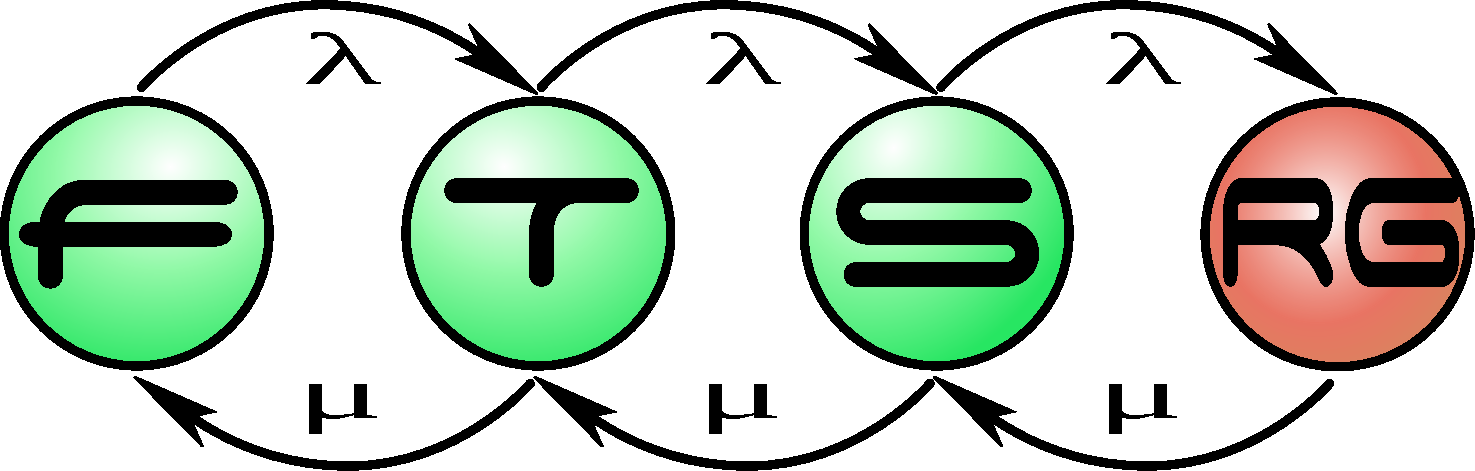
\includegraphics[width=60mm,keepaspectratio]{figures/ftsrg-logo}\\

\vfill

Bergmann Gábor \\
Darvas Dániel \\
Debreceni Csaba \\
Gönczy László \\
Farkas Rebeka \\
Molnár Vince \\
Salánki Ágnes \\
Semeráth Oszkár \\
Szárnyas Gábor \\
Tóth Tamás \\
Pataricza András \\
Vörös András

\vfill

{\large \today}

\vspace{3cm}
\end{center}
\end{titlepage}


%\vspace*{\fill}

{
\centering
Szerző:\\\textbf{}
	
\vspace*{\fill}

egyetemi oktatási célra

\vspace*{\fill}

Copyright © , 2016
\\
\\

Terjedelem: 20 (B5) ív\\
Nyomdai munkák:\\


}

\vspace*{\fill}%

\raggedbottom

\renewcommand{\thepage}{\roman{page}}

\cleardoublepage
\tableofcontents
\cleardoublepage
\renewcommand{\thepage}{\arabic{page}}

% Fejezetek közötti hivatkozáshoz sablon:
%\iflabeldef{sec:}{\aref{sec:}.~***ban}{a \emph{}}
% Példa:
%\iflabeldef{sec:modellek-ellenorzese}{\aref{sec:modellek-ellenorzese}.~fejezetben}{a \emph{Modellek ellenőrzése}}

\topic{Bevezető}

Vajon mennyi programkódot képes átlátni egy programozó? Hány sorból áll a Windows 7 forráskódja?\footnote{Körülbelül \href{http://www.fastcodesign.com/3021256/infographic-of-the-day/infographic-how-many-lines-of-code-is-your-favorite-app\#5}{40 millió sorból}.} Hogyan lehetséges mégis kézben tartani ekkora szoftverek fejlesztését? Hogyan garantálhatjuk, hogy a végső termék nem lesz hibás, megfelelő lesz a teljesítménye, és a rajta dolgozó mérnökökön kívül később más is képes lesz megérteni és módosítani a programot? Ezekre a kérdésre ad választ a Rendszermodellezés tárgy a komplex rendszerek modellezésének alapvető aspektusainak bemutatásával.

A \emph{modellezés} egy jól bevált technika a bonyolult rendszerek komplexitásának kezelésében. A tárgy célja ezért a hallgatók megismertetése a szoftver- és hardverrendszerek modellezésének eszközeivel és módszereivel. A modellezés alapfogalmainak bevezetése után a modellek két nagy csoportjával, a struktúra-alapú és viselkedés-alapú modellekkel foglalkozunk. Szó lesz a modellek fejlesztéséről, illetve az elkészült modellek ellenőrzéséről, különböző felhasználásairól is.

\begin{pelda}
	Vállalatunk a kezdeti sikereken felbuzdulva úgy dönt, hogy belép a közösségi taxizás piacára egy saját szolgáltatás indításával. Ehhez ki kell fejleszteni egy nagyméretű, elosztott rendszert, amelynek részét képezi majd a cég belső gépeire telepített központi szerver és a felhasználók okostelefonjain futó mobilalkalmazás, valamint kapcsolatban fog állni egy bank rendszerével is a fizetések lebonyolításához.
	
	A szenior szoftvermérnök a kezdetektől modellalapú fejlesztésben gondolkodik, hiszen a rendszer mérete és összetettsége több szempontból is indokolja a modellek használatát. Először is a tervezés első lépései során nem lenne szerencsés alacsony szintű technikai problémákkal foglalkozni. Egy megfelelően \emph{absztrakt} modell segítségével a részletkérdések kezdetben elhanyagolhatók, így a mérnökök elsőként a legfontosabb jellemzők kialakítására fókuszálhatnak.
	
	Mivel a megcélzott terület a cég számára új, mindenekelőtt a kapcsolódó fogalmak és a köztük húzódó összefüggések feltárása lesz a cél. A rendszer elosztottsága miatt szükség lesz az egyes összetevők (szerver, mobiltelefon, bank, hálózat stb.) kapcsolatainak modellezésére is. Az ezekhez szükséges eszközöket a \emph{struktúra alapú modellezés} nyújtja.
	
	Amint elkészül a rendszer architektúrája, a mérnökök nekiláthatnak az egyes komponensek viselkedésének tervezéséhez. Itt két kapcsolódó feladat is felmerül: meg kell tervezni a rendszer \emph{folyamatait} (pl. autórendelés, regisztráció, egyenleg feltöltése stb.), illetve ennek megvalósításához az egyes komponensek belső \emph{állapotait} és lehetséges állapotváltozásait. Az ezekhez szükséges eszközöket az \emph{viselkedés alapú modellezés} nyújtja.
	
	Természetesen a vezetőség szeretné elkerülni a tervezési hibák miatti többletköltségeket. A szenior mérnök javaslatára a megszokott \emph{tesztelésen} kívül már a rendszer modelljein is \emph{ellenőrzéseket} fognak végrehajtani, így a hibák azelőtt kiderülhetnek, hogy a tényleges implementációt (drága emberi erőforrás felhasználásával) elkészítenék.
	
	A szoftverek hibátlan működése mellett legalább ilyen fontos, hogy a rendszer \emph{teljesítménye} megfelelő legyen. Ha a szolgáltatásunk nem elérhető vagy lassan válaszol, a felhasználók minden bizonnyal a konkurenciához menekülnek majd, a vállalkozásunk pedig kudarcba fullad. Szerencsére a leendő rendszer teljesítménye is jól becsülhető a modellek alapján, ehhez a \emph{teljesítménymodellezés} nyújt majd eszköztárat.
	
	Részben ide tartozik az is, hogy a legtöbb viselkedésmodell \emph{szimulálható}. Ez több szempontból is a hasznunkra válik majd, hiszen egyrészt már a fejlesztés korai fázisában ki lehet próbálni az alapfunkciókat, másrészt a szimulációk eredményét is felhasználhatjuk a teljesítmény becslésére.
	
	Akár a szimulációkból, akár később az elkészült rendszer monitorozásából rengeteg információ is a rendelkezésünkre áll majd. Ahhoz, hogy ezekből használható tudást állítsunk elő, és adott esetben problémákat, vagy a rendszer rejtett tulajdonságait felfedezhessük, a \emph{felderítő adatelemzés} eszköztárát is bevethetjük majd.
	
	Korábban szóba került már a mindenek felett álló költséghatékonyság és a drága emberi erőforrás is. Szerencsére a szenior mérnöknek erre is van válasza: a kellően precíz modellekből akár \emph{kódot is generálhatunk}, amivel rengeteg mérnökórát spórolhatunk meg.
	
	Nincs más hátra, mint elküldeni a cégünk egyébként kiváló programozóit egy rendszermodellezés témájú tanfolyamra -- vagy felbérelni egy fejvadász céget az ilyen téren (is) jól képzett műegyetemisták levadászására...
\end{pelda}

%TODO: ezt az ígéretet lehet, hogy felül kell majd vizsgálni.
Ebben a jegyzetben a tárgyhoz tartozó legfontosabb témákat mutatjuk be. Az alapfogalmak definícióit releváns mérnöki példákkal illusztráljuk és magyarázzuk, illetve gyakorló feladatokkal segítjük a bemutatott módszerek megértését.
Ehhez különböző színű keretes írásokat fogunk használni. Amint az előzőekben látszott, a példák narancssárga háttérrel jelennek meg. A definíciók sárga háttérrel kerülnek kiemelésre, míg a kiegészítő megjegyzések szürke színt kapnak. A jegyzetben szerepelnek majd feladatok is piros háttérrel, valamint hasznos tippek zöld keretben.

\begin{definicio}
	A \emph{definíció} egy fogalom pontos, precíz meghatározása.
\end{definicio}

\begin{megjegyzes}
	Időnként megjegyzésekkel fogjuk árnyalni a bemutatott anyagot.
\end{megjegyzes}

\begin{feladat}
	Gyakorlásképp oldja meg az egyes fejezetekhez tartozó feladatokat!
\end{feladat}

\begin{tipp}
	A feladatokhoz hasonló kérdések előfordulhatnak a számonkéréseken is.
\end{tipp}

\section*{A jegyzetről}

A jegyzet \LaTeX\ nyelvű forráskódja elérhető a \url{https://github.com/FTSRG/remo-jegyzet} oldalon.

A jegyzet jelenleg fejlesztés alatt áll. Amennyiben az elkészült részekben hibát vagy hiányosságot találtok, kérjük jelezzétek a GitHubon egy új \emph{issue} felvételével. Amennyiben javítási ötletetek van, örömmel fogadjuk a \emph{pull requesteket} is.

% !TeX spellcheck = hu_HU
\topic{Modellezés és metamodellezés}

\graphicspath{ {./modellezes-es-metamodellezes/figures/} }

Ebben a fejezetben a modellezés alapfogalmaival fogunk megismerkedni. Az itt bevezetett fogalmak újra és újra megjelennek majd a későbbi fejezetekben, ahol részletesen ki fogunk térni az adott területen történő értelmezésükre.

%Az alábbi dokumentum a rendszermodellezés tárgy első előadásához kapcsolódó segédanyag, mely tartalmazza az elhangzott definíciókat és a hozzájuk tartozó egyszerűbb magyarázatokat.

\section{Modellezés}

Mi értelme van modellezni? Fejben szinte mindig modellezünk, bármilyen probléma kerül elénk. Nincs ez másképp egy szoftver fejlesztésekor sem. Lássuk hát, miről beszélünk, amikor a modell szót használjuk.
% Legfőbb szerepe a kommunikáció:

\begin{definicio}
	\Fogalom{modell}: egy valós vagy hipotetikus világ (a ,,\fogalom{rendszer}'') egy részének egyszerűsített képe, amely a rendszert helyettesíti bizonyos megfontolásokban. Egy modell elkészítésének mindig egy kérdés megválaszolása a célja.
\end{definicio}

A modell tehát egy többnyire bonyolult rendszer egyszerűsített reprezentációja, amiben csak az aktuális probléma szempontjából lényeges vonásokat szerepeltetjük.
Egy adott rendszer modellé történő leképezésének általában két fontos előnye van: %\emph{áttekinthetőbb}, \emph{kisebb (véges)}.

\begin{itemize}
	\item A modell az eredeti rendszernél \emph{kisebb}, hiszen az aktuális problémához nem (vagy lazábban) kapcsolódó, elhanyagolható információk nem jelennek meg benne.
	\item A modell az eredeti rendszernél \emph{áttekinthetőbb}, hiszen csak az adott probléma szempontjából érdekes, releváns információkat és kapcsolatokat kell vizsgálni.
\end{itemize}

\begin{pelda}
	Modellekre sok példát láthatunk a hétköznapokban is. Nem csak gyerekek körében népszerű játék a modellvasút. Itt valóban modellről beszélhetünk, hiszen a játékvonatok számos tekintetben hűen reprezentálják a valódi vonatokat, azonban például ``szemet hunyunk'' a méretükkel, tömegükkel, a bennük lévő villanymotor paramétereivel és még sok egyéb hasonló tulajdonságukkal kapcsolatban.

	Az informatika egyik leggazdagabb modellforrása a matematika. Amikor gráfelméletet tanulunk, valójában rengeteg, bizonyos szempontból hasonló probléma közös modelljét vizsgáljuk. Valóban, a matematika egyik célja az ilyen modellek azonosítása és minél hatékonyabb eszköztárak kidolgozása a rajtuk megfogalmazott feladatok megoldására. A gráfoknál maradva (gráfokról bővebben \iflabeldef{sec:graf}{\aref{sec:graf}.~szakaszban}{a \emph{Struktúra alapú modellezés} c. segédanyagban} és a \bszketto c. tárgyban lehet tájékozódni) egy város úthálózata jól reprezentálható egy élsúlyokkal ellátott gráffal, ahol a csomópontok a kereszteződések, az élek az útszakaszok, az élsúlyok pedig a szakaszok hosszait jelölik. Ez a modell kiválóan alkalmas legrövidebb útvonalak tervezésére (mi kellene még a \emph{leggyorsabb} útvonal tervezéséhez?), de figyelmen kívül hagy számos egyéb paramétert, például az utakon lévő kanyarulatokat, a legnagyobb megengedett sebességet stb.
\end{pelda}

\begin{megjegyzes}
	Az, hogy a modell kisebb, nem mindig ``kényelmi'' szempont. Gyakran lehet olyan problémával találkozni, aminek a mérete bizonyos szempontból \fogalom{vegtelen} (például végtelen sok állapota van, folytonos változók vannak benne, esetleg részét képezi az \emph{idő}), viszont egy alkalmas \fogalom{veges} modellen a számunkra releváns tulajdonságok továbbra is jól vizsgálhatók maradnak. Egy autót fizikai szempontból modellezhet a pillanatnyi sebességvektora, ami három valós szám, tehát a modellünk így végtelen. Ha viszont feltételezzük, hogy a sebesség nagysága nem lehet $200~\textrm{km/h}$-nál több, és két tizedesjegy pontossággal adjuk meg a vektor koordinátáit (tehát \emph{diszkrét értékekkel} jellemezzük a rendszert), akkor máris véges modellt kapunk. Természetesen ez a modell kicsit torzítani fog a valósághoz képest, de számos problémánál ez a hiba elhanyagolhatóan kicsi lesz (ráadásul végtelen modellen lehet, hogy nem is tudnánk megoldást adni).
\end{megjegyzes}

Fontos kérdés, hogy hogyan lehet ábrázolni egy modellt. Maga a modell ugyanis többnyire egy hipotetikus struktúra, nem kézzel fogható és nem is mindig célszerű teljes részletességgel ábrázolni.

\begin{definicio}
	\Fogalom{diagram}: a modell egy nézete, amely a modell bizonyos aspektusait grafikusan ábrázolja.
\end{definicio}

\begin{megjegyzes}
Fontos megjegyezni, hogy nem minden modell, ami modellnek látszik.

\begin{itemize}
	\item \emph{A modell nem a valóság}: az általunk definiált modellen bizonyos állítások igazak lehetnek, amik a valóságban nem állják meg a helyüket.
	\item \emph{A modell nem a diagram}: a diagram csak egy ábrázolás módja a modellnek, amivel olvashatóvá tesszük.
\end{itemize}
\end{megjegyzes}

%\todo{<első alternatíva>}
%
%\section{Modellezési nyelvek}
%
%A modellek leírásához nem elég, ha diagramokat rajzolunk. Egy modell precíz megadásához szükség van egy \fogalomragozva{modellezesi nyelv}{modellezési nyelvre}. Egy modellezési nyelv lehet \emph{szöveges} (pl. Verilog, VHDL, Java stb.) vagy \emph{grafikus} (pl. webes konyhatervező, UML diagramok stb.). Gyakori, hogy egy modell leírásához szöveges és grafikus nyelvet is használunk, ugyanis mindkettőnek megvannak a saját előnyei és hátrányai: jellemzően modellt építeni könnyebb szöveges nyelv használatával, míg a modell olvasása grafikus nyelvek (diagramok) segítségével egyszerűbb.
%
%A modellezési nyelvek legfőbb célja a kommunikáció gép-gép, ember-gép, vagy akár ember-ember között is. Egy nyelv megadásához két dolgot kell definiálni: a \emph{szintaxist} és a \emph{szemantikát}.
%
%%Segítségükkel modelleket építhetünk, amik lehetnek szöveges (pl.: Verilog, VHDL, Java stb.), vagy grafikusak is (pl.: webes konyhatervező, UML diagrammok, UPPAAL stb.). Céljuk a kommunikáció gép-gép, ember-gép vagy akár ember-ember között is. A nyelveknek két fő aspektusa van:
%
%\begin{definicio}
%	\Fogalom{szintaxis}: egy szabályrendszer, ami meghatározza, hogy a modell milyen elemekből épül fel, ezeknek mi a (szöveges vagy grafikus) reprezentációja, és a különböző elemek milyen módon kombinálhatók.
%\end{definicio}
%
%\begin{definicio}
%	\Fogalom{szemantika}: a szintaxis által megadott nyelvi elemek jelentését definiáló szabályrendszer.
%\end{definicio}
%
%%\begin{itemize}
%%	\item \fogalom{szintaxis}: hogyan írom a le a modellt? Egy szabályrendszer, ami meghatározza, hogy a nyelv milyen elemekből épül fel és azok hogyan kombinálhatóak.
%%	\item \fogalom{szemantika}: mit jelent a modell? A szintaxis által definált nyelvi elemek jelentését definiáló szabályrendszer.
%%\end{itemize}
%
%A szintaxis tehát definiálja, hogy hogyan írhatjuk le a modellt az adott nyelv segítségével, a szemantika pedig megadja, hogy az így leírt modell pontosan mit jelent.
%
%\begin{pelda}
%	A C nyelv egy szöveges nyelv, melyben elemeknek tekinthetjük az \code{if}, \code{for}, \code{switch}, \code{változónevek}, \code{metódusnevek}, \code{típusok} stb. részeket. Ezek azonban nem tetszőleges sorrendben állhatnak egymás mellett, hanem egy jól meghatározott szabályrendszer szerint. Ez a szintaxis. Azt, hogy az \code{if} kulcsszóval elágazást, a \code{for} kulcsszóval pedig egy ciklust definiálunk és nem pedig valami teljesen más dolgot, a szemantika határozza meg. Vagyis a szemantika jelentéssel tölti meg a nyelvi elemeket.
%
%	A Yakindu eszköz bizonyos szinten egy grafikus nyelvet határoz meg, ahol például nyelvi elemek a dobozok és nyilak (az állapottérképek Yakindu által definiált modellezési nyelvét \iflabeldef{sec:allapot-alapu-modellezes}{\aref{sec:allapot-alapu-modellezes}.}{az \emph{Állapot alapú modellezés}}). A szintaxis meghatározza, hogy a dobozokból csak nyilakkal lehet összekötni más dobozokat. A szemantikus jelentésük pedig az, hogy a dobozok állapotokat, a nyilak pedig állapotátmeneteket jelölnek (tehát megmutatják, hogy az alkalmazásunk melyik állapotból melyik állapotba kerülhet).
%\end{pelda}
%
%\begin{megjegyzes}
%	Szintaktikailag leírhatunk olyan kifejezéseket a nyelvben, aminek szemantikailag nincs értelme: jó példa erre a nullával osztás.
%\end{megjegyzes}
%
%
%\section{Metamodellezés}
%
%Az imént bevezetett modellezési nyelvek szerepe az volt, hogy modelljeink leírhatóak, megjeleníthetőek legyenek. Azt is mondtuk, hogy ugyanazt a modellt többféle nyelven is érdemes lehet reprezentálni. Ez viszont azt jelenti, hogy egy adott modelltípus leírására alkalmas nyelvek mögött van egy közös \emph{modell}, ami miatt alkalmasak ugyanannak az ismeretnek a kifejezésére.
%
%\begin{definicio}
%	A \fogalom{metamodell} egy modellezési nyelv modellje. Meghatározza, hogy a nyelvnek milyen típusú elemei vannak, milyen kapcsolatban állhatnak egymással, és a típusoknak mi a viszonya egymáshoz.
%\end{definicio}
%
%A metamodell tehát modellezési nyelveket modellez, a konkrét jelölölésrendszer elhanyagolásával. A metamodellt emiatt szokás \fogalomragozva{absztrakt szintaxis}{absztrakt szintaxisnak} is nevezni, míg a korábbiakban definiált szintaxisra ilyenkor \fogalomragozva{konkret szintaxis}{konkrét szintaxisként} szokás hivatkozni. Ezzel a terminológiával élve egy modellezési formalizmust az absztrakt szintaxisával (más néven egy metamodellel), egy vagy több konkrét szintaxissal (szöveges vagy grafikus jelölésrendszer a metamodell elemeihez) és a szemantikával adhatunk meg.
%
%\begin{pelda}
%	Modellekre és metamodellekre számos példa kerül majd elő a későbbi tanulmányok során:
%	\begin{itemize}
%		%\item Egyed-kapcsolat, EK modell (entity-relationship, ER)
%		\item AZ UML~\cite{UML} (Unified Modeling Language) objektum diagramján ábrázolt objektummodelleket az osztálydiagramokon ábrázolt metamodelljeik szerint adhatjuk meg.
%		\item Egy adatbázis tábla metamodellje a relációs adatbázisséma.
%		\item Az XML dokumentumok metamodelljét az XML sémák adják.
%	\end{itemize}
%	A konkrét szintaxist (jelölésrendszert) mindegyik esetben külön határozzák meg, az UML esetében többféle grafikus és szöveges szintaxis is definiált.
%\end{pelda}
%
%\begin{tipp}
%	Minden fejezetben, ahol modellezési formalizmusokkal ismerkedünk meg, szerepelni fog az adott adott modelltípus metamodellje is.
%\end{tipp}
%
%\todo{</első alternatíva>}
%\todo{<második alternatíva>}

\section{Modellezési nyelvek}

A modellek leírásához nem elég, ha diagramokat rajzolunk. Egy modell precíz megadásához szükség van egy \fogalomragozva{modellezesi nyelv}{modellezési nyelvre}. A modellezési nyelvek legfőbb célja a kommunikáció gép-gép, ember-gép, vagy akár ember-ember között is. Egy modellezési nyelv lehet \emph{szöveges} (pl. Verilog, VHDL, Java stb.) vagy \emph{grafikus} (pl. webes konyhatervező, UML diagramok stb.). Gyakori, hogy egy modellezési nyelv szöveges és grafikus jelölésrendszert is definiál, ugyanis mindkettőnek megvannak a saját előnyei és hátrányai: jellemzően modellt építeni könnyebb szöveges nyelv használatával, míg a modell olvasása grafikus nyelvek (diagramok) segítségével egyszerűbb.

\begin{definicio}
	Egy \fogalom{modellezesi nyelv} négy részből áll:
	\begin{itemize}
		\item \Fogalom{absztrakt szintaxis} (más néven \fogalom{metamodell}): meghatározza, hogy a nyelvnek milyen típusú elemei vannak, az elemek milyen kapcsolatban állhatnak egymással, és a típusoknak mi a viszonya egymáshoz. Ezt a reprezentációt használják gépek a modell belső tárolására.
		\item \Fogalom{konkret szintaxis}: az absztrakt szintaxis által definiált elemtípusokhoz és kapcsolatokhoz szöveges vagy grafikus jelölésrendszert definiál. Ezt a reprezentációt használják az emberek a modell olvasására és szerkesztésére.
		\item \Fogalom{jolformaltsagi kenyszer}: Megadja, hogy egy érvényes modellnek milyen egyéb követelményeknek kell megfelelnie.
		\item \Fogalom{szemantika}: az absztrakt szintaxis által megadott nyelvi elemek jelentését definiáló szabályrendszer.
	\end{itemize}
	Egy modellezési nyelvhez több konkrét szintaxis is adható.
\end{definicio}

Az absztrakt szintaxis tekinthető a modellezési nyelv modelljének, ezért hívjuk \emph{metamodellnek} is. A konkrét szintaxis a metamodellhez képest annyival több, hogy a definiált elemekhez megjeleníthető reprezentációkat rendel, ezáltal válik olvashatóvá és szerkeszthetővé egy modell leírása. Ha nem okoz félreértést, akkor a szintaxis szót leggyakrabban az absztrakt és konkrét szintaxis együttes jelölésére használjuk (tehát az elemkészletre és a jelölésekre együtt). A jólformáltsági kényszerek tovább szűkítik a lehetséges modellek körét olyan szabályokkal, mint például az azonos nevű elemek tiltása. Végül a szemantika megadja, hogy az így leírt modell pontosan mit is jelent, vagy hogyan ``működik''. A szemantika fogalmát strukturális és viselkedési modellek esetén kissé eltérően értelmezzük majd, erre a későbbi fejezetekben térünk vissza.

\begin{pelda}
	A C nyelv egy szöveges nyelv, melyben elemeknek tekinthetjük az \code{if}, \code{for}, \code{switch}, \code{változónevek}, \code{metódusnevek}, \code{típusok} stb. részeket. Ezek azonban nem tetszőleges sorrendben állhatnak egymás mellett, hanem egy jól meghatározott szabályrendszer szerint. Ez a szintaxis. Azt, hogy az \code{if} kulcsszóval elágazást, a \code{for} kulcsszóval pedig egy ciklust definiálunk és nem pedig valami teljesen más dolgot, a szemantika határozza meg. Vagyis a szemantika jelentéssel tölti meg a nyelvi elemeket.
\end{pelda}

\begin{pelda}
	A Yakindu Statechart Tools\footnote{\url{http://statecharts.org}} egy állapotgépek specifikálását és fejlesztését lehetővé tévő nyílt forráskódú eszköz, mely az Eclipse IDE alapjaira épül. Kényelmi funkcióihoz tartozik az elkészített modell validációja, szimulálásának lehetősége, ill. a modellalapú kódgenerálás is. A szöveges (XML) nyelv mellett egy könnyen használható grafikus felületet is biztosít, ahol lehetőségünk van állapotokat és átmeneteket definiálni. Ezek nyelvi elemként, mint dobozok és nyilak jelennek meg. A grafikai szintaxis meghatározza, hogy a dobozokból csak nyilakkal lehet összekötni más dobozokat. Ekkor igazából azt adjuk meg, hogy egy adott állapotból alkalmazásunk milyen másik állapotba kerülhet. Ez a szemantikai jelentés. Az állapot alapú modellek leírásával részletesen \iflabeldef{sec:allapot-alapu-modellezes}{\aref{sec:allapot-alapu-modellezes}.}{az \emph{Állapot alapú modellezés}} fejezetben fogunk foglalkozni.
\end{pelda}

\begin{megjegyzes}
	A metamodell ugyanúgy modell, mint a segítségével leírható modellek. Ebből kifolyólag ugyanúgy adható hozzá modellezési nyelv, aminek szintén lesz egy metamodellje. A gyakorlatban ez addig folytatódik, amíg az egyik metamodellt már egy szabványos modellezési nyelv segítségével írjuk fel. Érdekesség, hogy az UML metamodell-hierarchiájának gyökerében egy \emph{önleíró modell} található: önmaga a saját metamodellje is egyben.
\end{megjegyzes}

\begin{pelda}
	Modellekre és metamodellekre számos példa kerül majd elő a későbbi tanulmányok során:
	\begin{itemize}
		%\item Egyed-kapcsolat, EK modell (entity-relationship, ER)
		\item Az \rovidites{UML}~\cite{UML} objektum diagramján ábrázolt objektummodelleket az osztálydiagramokon ábrázolt metamodelljeik szerint adhatjuk meg (\szofttech tárgy).
		\item Az \rovidites{XML} dokumentumok metamodelljét az XML sémák adják (\szofttech tárgy).
		\item Egy adatbázis tábla metamodellje a relációs adatbázisséma (\adatb tárgy).
	\end{itemize}
	A konkrét szintaxist (jelölésrendszert) mindegyik esetben külön határozzák meg, az UML esetében többféle grafikus és szöveges szintaxis is definiált.
\end{pelda}

\begin{tipp}
	Minden fejezetben, ahol modellezési formalizmusokkal ismerkedünk meg, szerepelni fog az adott modelltípus metamodellje is.
\end{tipp}

%\todo{</második alternatíva>}

\section{Nyílt és zárt világ feltételezés} \label{sec:owacwa}

Egy modell szemantikájának definiálása során több feltételezésből is kiindulhatunk. Ezeket rögzíteni kell, és a modell értelmezésekor döntő szerepük van a különböző állítások igazságtartalmának eldöntésekor.

\begin{definicio}
	\Fogalom{zart-vilag-feltetelezes}: Minden állítás, amiről nem ismert, hogy igaz, hamis.
\end{definicio}

\begin{definicio}
	\Fogalom{nyilt-vilag-feltetelezes}: Egy állítás annak ellenére is lehet igaz, hogy ez a tény nem ismert.
\end{definicio}

A két feltételezés között az egyik legfontosabb különbség, hogy a nyílt világ feltételezés elismeri és használja az \emph{ismeretlen} fogalmát, míg a zárt világban minden tudás ismertnek tekintett. Mindkét feltételezésnek megvan a maga szerepe és helye, ahogy azt a következő két példa is illusztrálja.

\begin{pelda}
	A zárt világ feltételezést olyankor alkalmazzuk, amikor egy rendszernek a teljes szükséges információ a rendelkezésére áll. Erre példa egy tömegközlekedési adatbázis: ha megkérdezzük, hogy közlekedik-e közvetlen járat a Magyar Tudósok körútja és a Gellért tér között, és ilyen járat nincs az adatbázisban, akkor a válasz egyértelmű ``nem''. Ebben az esetben valóban ez az elvárt és helyes válasz.

	A nyílt világ szemantika olyankor alkalmazandó, amikor nem feltételezhetjük, hogy minden információ a rendelkezésünkre áll. Például egy orvosi nyilvántartó rendszerben előfordulhat (sőt, számítani kell rá), hogy egy beteg annak ellenére allergiás valamire, hogy ez a nyilvántartásban nem szerepel.
\end{pelda}

\section{Absztrakció és finomítás}

A modell definíciójának szerves része az \emph{egyszerűsítés}, az adott probléma szempontjából irreleváns információk elhanyagolása. Ugyanannak a rendszernek több modelljét is elkészíthetjük más-más részletek kihagyásával. Ráadásul egy elkészített modellből további részleteket hagyhatunk el, vagy éppen újabb részleteket vehetünk bele, így a modellek a részletgazdagság szerint egyfajta hierarchiába rendezhetők.

Különbséget kell tennünk azonban egy modell részletekkel gazdagítása és megváltoztatása között. Ehhez segít, ha megkülönböztetjük a modellt (illetve a modellezett rendszert) és a környezetét.

\begin{definicio}
	\Fogalom{rendszer} és \fogalomragozva{kornyezet}{környezete}: a környezet (vagy kontextus) a rendszerre ható tényezők összessége. Modellezéskor a modellezett rendszernek mindig egyértelműen definiálni kell a \emph{határait}. A határon belül eső dolgokat a rendszer részének tekintjük, az azon kívül esők adják a környezetet. Szokás még a környezet elemeit két csoportba sorolni: \emph{releváns} környezeti elemek azok a dolgok, amik a rendszerrel közvetve vagy közvetett módon kapcsolatban állnak, míg \emph{irreleváns} környezeti elem, ami a rendszerrel nincs kapcsolatban.
\end{definicio}

\begin{megjegyzes}
	Gyakori, hogy egy rendszer környezetéről (is) készítünk modelleket. Ennek haszna a rendszer és a környezet interakcióinak pontosabb megértése, tervezése és analízise. Az elkészült rendszerek tesztelésekor például gyakran nem az éles környezetben tesztelünk, hanem a környezet modellje alapján szimuláljuk az interakciókat.

	A környezet szempontjából nézve a rendszert tekinthetjük \fogalomragozva{fekete doboz}{fekete doboznak} vagy \fogalomragozva{feher doboz}{fehér doboznak}. Előbbi esetben a rendszer belső felépítését és viselkedését nem ismerjük, míg utóbbi esetben ezek az információk rendelkezésre állnak. Ez a két fogalom főleg tesztek tervezésekor érdekes, erről bővebben \iflabeldef{sec:modellek-ellenorzese}{\aref{sec:modellek-ellenorzese}.~fejezetben}{a \emph{Modellek ellenőrzése}} fejezetben lesz szó.
\end{megjegyzes}

\begin{pelda}
	Sportautók tervezésekor a rendszer jól körülhatárolható. Aerodinamikai szempontból releváns külvilágnak tekinthető az autó körül áramló levegő. Tervezéskor célszerű a karosszéria (rendszer) és a légáramlás (környezet) modelljét is elkészíteni, hogy minél pontosabb szimulációkkal megfelelő jóslatokat tudjunk tenni a terv minőségét illetően. Később, amikor az elkészült prototípus tesztelése folyik, a szélcsatorna tekinthető a légáramlás egy pontosabb, fizikai modelljének.
\end{pelda}

A környezet segítségével definiálhatjuk, hogy mit jelent a modell részletekkel gazdagítása.

\begin{definicio}
	\Fogalom{finomitas}: a modell olyan részletezése (pontosítása), hogy a környezet szempontjából nézve a finomított modell (valamilyen tekintetben) helyettesíteni tudja az eredeti modellt.
\end{definicio}

A finomítás mindig többletismeret bevitelét jelenti a modellbe. A finomítás konkrét módja és a helyettesíthetőség pontos definíciója problémafüggő, amikre sok példát láthatunk majd a későbbi fejezetekben. Természetesen a finomításnak ellentétes művelete is van.

\begin{definicio}
	\Fogalom{absztrakcio}: a finomítás inverz művelete, vagyis a modell részletezettségének csökkentése, a modellezett ismeretek egyszerűsítése.
\end{definicio}

A szabályos finomítás után az eredeti modell mindig visszakapható egy szabályos absztrakcióval. Érdemes megjegyezni, hogy finomítás során többnyire tervezői döntést hozunk annak tekintetében, hogy egy adott részletet hogyan illesztünk a modellbe, míg az absztrakció során a részlet elhagyása egyértelmű. Következésképpen egy finomítási lépésnek általában sokféle eredménye lehet, de egy adott absztrakciós lépésnek mindig csak egy.

\begin{pelda}
	Egy közlekedési lámpának megadható egy absztrakt és egy részletes modellje is. Az absztrakt modellben a lámpának két állása van: \emph{tilos} és \emph{szabad}. A részletesebb modellben a \emph{szabad} állapotnak megfelelhet a \emph{zöld} állapot, a \emph{tilos} állapotban pedig a \emph{sárga}, \emph{piros} és \emph{piros-sárga}.

	Figyeljük meg, hogy az absztrakt modellből a részletesebbe lépés (finomítás) során többlet ismeretet vittünk a modellbe, mégpedig a lámpákkal kapcsolatban. Ráadásul mivel az új állapotok mindegyike egyértelműen megfeleltethető egy réginek, a környezet számára a rendszer továbbra is leírható az absztrakt modellel.

	Azt is láthatjuk, hogy a finomítási lépésnek (``bontsuk szét a \emph{tilos} állapotot'') több megoldása is lehetett volna, míg az ennek megfelelő absztrakciós lépésnek (``vonjuk össze a \emph{sárga}, \emph{piros} és \emph{piros-sárga} állapotokat'') csak egyetlen megoldása van (az elnevezésektől eltekintve).
\end{pelda}

\begin{tipp}
	A későbbi fejezetekben az adott témakör vonatkozásában számos példát adunk majd absztrakcióra és finomításra.
\end{tipp}

\topic{Struktúra alapú modellezés}

\graphicspath{ {./struktura-alapu-modellezes/figures/} }

\newcommand{\yedscale}{0.7}

% vezérpélda lehetőségek
% - táblázatszerű adatok pl. felhasználókról (preferenciák, van-e jogsija, stb.), kocsikról (férőhely, légkondi stb.)
% - kiszolgáló rendszer top-down, bottom-up tervezése (mobil kliens, tömegközl. integráció, adatbázis stb.)
% - gráfként reprezentált fuvarok, kocsik, szakaszok, utasok, sofőrök stb.

%\begin{megjegyzes}
%	kifejteni azt, hogy lehet logikai és fizikai felépítés alapján is modellezni.
%	
%	- Fizikai/architektúrális egységek --> moduláris struktúra hoz létre, újrahasznosítható részekkel.
%	
%	- Funkcionális egységek --> dedikált struktúrát hoz létre, pl. távirányító -- redundanciamentes, azért, hogy a költség alacsony legyen. Nem újrahasznosíthatók a részei.
%	
%	Pl. dedikált eszközt készítünk, amikor van egy rendszermenedzsment problémám és írok rá egy szkriptet. A másik megoldás lenne, hogy behozunk egy rendszermenedzsment eszközt és annak az újrahasznosítható komponenseit alkalmazzuk.
%	
%	Jó lenne építészeti példát behozni.
%\end{megjegyzes}

Hogyan épül fel egy rendszer? Milyen részekre bontható és ezek között milyen kapcsolat van? Ahhoz, hogy a rendszerünkkel kapcsolatos problémákat megválaszoljuk, fontos, hogy ezekre a kérdésekre tudjuk a választ. Ebben a fejezetben az egyes rendszerek \fogalomragozva{struktura}{struktúrájának} jellemzésével foglalkozunk. Bemutatjuk a strukturális modellezés motivációját, a leggyakrabban alkalmazott formalizmusokat és azok matematikai alapjait.

%Modellezés során egy rendszert jellemezhetünk annak statikus, ill. dinamikus jellemzői alapján. A statikus jellemzés esetén a rendszer felépítését, \fogalomragozva{struktura}{struktúráját} írjuk le, míg dinamikus jellemzés esetén a rendszer \fogalomragozva{viselkedes}{viselkedésével} foglalkozunk.

%\clearpage

%%%%%%%%%%%%%%%%%%%%%%%%%%%%%%%%%%%%%%%%%%%%%%%%%%%%%%%%%%%%%%%%%%%%%%%%%%%%%%%%

\section{A struktúramodellezés alkalmazásai}
\label{sec:motivacio}

Mind a természetben, mind a mesterséges rendszerekben fellelhetők bizonyos szabályszerűségek. Egyes szabályszerűségek a rendszer elemei közötti kapcsolatokat, míg mások magukat az elemeket jellemzik. Bár sok mindenben eltér egy közlekedési hálózat, egy számítógép-hálózat, egy épület vagy egy város felépítése, a struktúramodellezés eszköztárával olyan ,,nyelvet'' kapunk, amivel ezeket hasonlóan modellezhetjük.

\subsection{Hálózatok}
\label{sec:halozatok}

Egy rendszert gyakran úgy jellemezhetünk a legjobban, ha bizonyos elemeit megkülönböztetjük és leírjuk az ezek közötti \fogalomragozva{kapcsolat}{kapcsolatot}.

\begin{pelda}
	Egy nagyváros közlekedési hálózata szövevényes rendszere az út- és sínhálózatnak, a több százezernyi járműnek és az ezeken utazó embereknek. A közlekedők mozgása mellett az infrastruktúra is folyamatosan változik a különböző fejlesztések, átalakítások és karbantartások miatt.
	
	Egy ilyen rendszer precíz modellezése lehetetlen vállalkozás lenne, ezért helyette tipikusan olyan absztrakciókkal dolgozunk, amik az adott probléma megoldásához szükséges információkat tartalmazzák. Például az útvonalkereső alkalmazások ismerik a helyi tömegközlekedés járatait és segítséget nyújtanak abban, hogy az indulási pontunktól a célállomásig közlekedő járműveket és az azok közötti átszállási lehetőségeket listázzák.
	
	Vizsgáljuk meg például Budapest metróhálózatát! Az egyszerűség kedvéért a példában a hálózatnak csak a Nagykörúton belüli részével foglalkozunk.
\end{pelda}

A metróhálózat egyszerűsített térképe \aref{fig:metrohalozat-nagykorut-terkep} ábrán látható. A térképből is látható, hogy a hálózat könnyen ábrázolható egy \fogalomragozva{graf}{gráffal}, ahol a gráf minden \fogalomragozva{csomopont}{csomópontja} egy-egy metróállomást jelöl. A csomópontok címkéje a metrómegálló neve. Két csomópont között akkor fut \fogalom{el}, ha a két megálló közvetlenül össze van kötve metróval. A metróhálózatot modellező %\fogalomragozva{iranyitatlan-graf}{irányítatlan}, \fogalomragozva{cimkezett-graf}{címkézett}, \fogalom{egyszeru-graf}
gráf \aref{fig:metrohalozat-nagykorut-egyszeru} ábrán látható.

\begin{figure}[H]
	\begin{subfigure}[b]{0.5\textwidth}
		\centering
		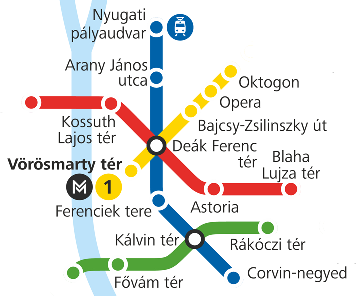
\includegraphics[width=0.9\textwidth]{metrohalozat-nagykorut-terkep}
		\caption{A metróhálózat térképe~\cite{BKK:metro}}
		\label{fig:metrohalozat-nagykorut-terkep}
	\end{subfigure}
	~
	\begin{subfigure}[b]{0.5\textwidth}
		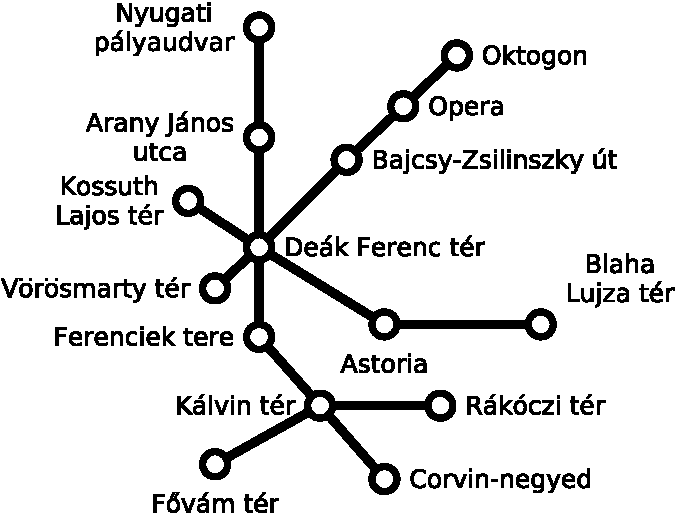
\includegraphics[width=\textwidth]{metrohalozat-nagykorut-egyszeru}
		\caption{A metróhálózat egyszerű gráfként ábrázolva}
		\label{fig:metrohalozat-nagykorut-egyszeru}
	\end{subfigure}
	\caption{Budapest metróhálózata a Nagykörúton belül}\label{fig:animals}
\end{figure}

A modellünk segítségével választ kaphatunk például a következő kérdésekre:

\begin{enumerate}
	\item Milyen megállók érhetők el a Vörösmarty térről indulva?
	
		Vizsgáljuk meg, hogy a Vörösmarty teret reprezentáló csomópontból kiindulva milyen csomópontok érhetők el. Ehhez elemi gráfbejáró algoritmusok használunk.
		
		\begin{megjegyzes}
			Elemi útkereső algoritmusok pl. a \roviditesmagyarul{BFS} vagy \roviditesmagyarul{DFS}.
		\end{megjegyzes}
	\item Legalább hány megállót kell utaznunk a Kossuth Lajos tér és a Kálvin tér között?

		A legrövidebb utat szintén kereséssel határozhatjuk meg.
		
		\begin{megjegyzes}
			Például egy \fogalomragozva{BFS}{szélességi kereséssel}.
		\end{megjegyzes}

\end{enumerate}

Vannak azonban olyan metróközlekedéssel kapcsolatos kérdések, amelyekhez a modell nem tartalmaz elég információt:

\begin{enumerate}
	\item Milyen megállók érhetők el a Fővám térről indulva \emph{legfeljebb egy átszállással}?
	\item A menetrend szerint \emph{hány percig tart} az út a Kossuth Lajos tér és az Astoria között?
\end{enumerate}

Ezeknek a kérdéseknek megválaszolásához egészítsük ki a gráfot! Az első kérdéshez szükséges, hogy az egyes metróvonalakat meg tudjuk különböztetni, amit például az élek címkézésével érhetünk el. \Aref{fig:metrohalozat-nagykorut-elcimkezett} ábrán színekkel jelöltük a különböző élcímkéket. Induljunk ki a Fővám térről: átszállás nélkül az Astoria és a Rákóczi tér megállókat érhetjük el, míg egy átszállással elérhetjük az M3-as metró vonalán található megállókat is.

\begin{figure}[H]
	\begin{subfigure}[b]{0.5\textwidth}
		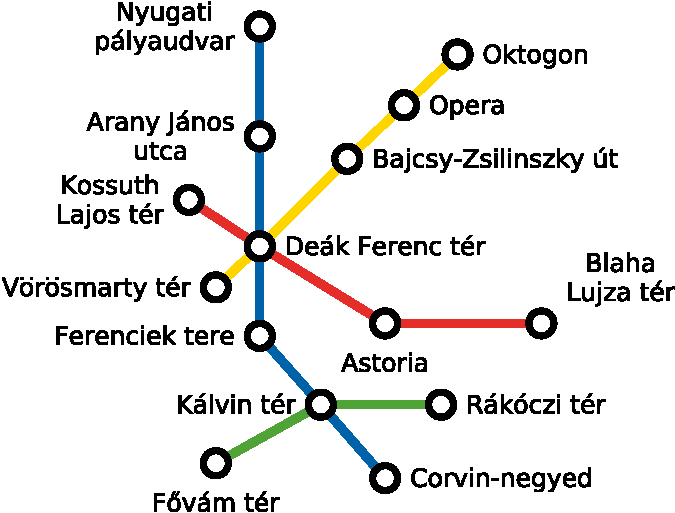
\includegraphics[width=\textwidth]{metrohalozat-nagykorut-elcimkezett}
		\caption{A gráf élcímkékkel kiegészítve}
		\label{fig:metrohalozat-nagykorut-elcimkezett}
	\end{subfigure}
	~
	\begin{subfigure}[b]{0.5\textwidth}
		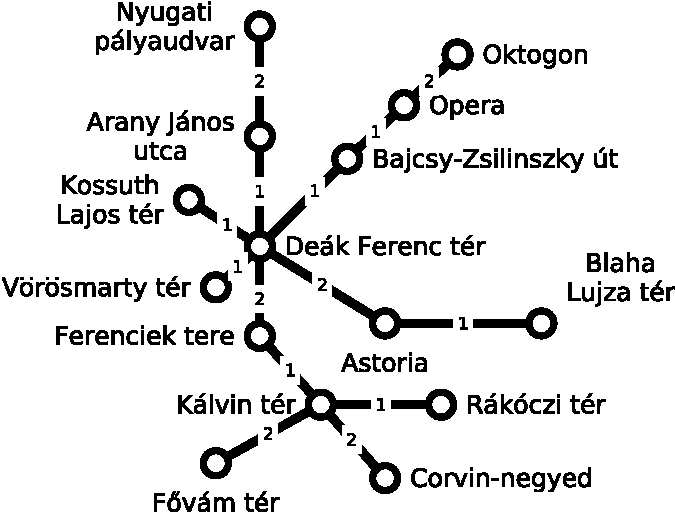
\includegraphics[width=\textwidth]{metrohalozat-nagykorut-elsulyozott}
		\caption{A gráf élsúlyokkal kiegészítve}
		\label{fig:metrohalozat-nagykorut-elsulyozott}
	\end{subfigure}
	\caption{A metróhálózatot ábrázoló gráf kiterjesztései}\label{fig:animals}
\end{figure}

A második kérdés megválaszolásához az egyes megállók közötti útidőt kell jellemeznünk. Ehhez vegyünk fel \fogalomragozva{elsuly}{élsúlyokat} a gráfba. \Aref{fig:metrohalozat-nagykorut-elsulyozott} ábrán élsúlyokkal jelöltük az egyes megállók között menetidőt. Ezek ismeretében meghatározható a Kossuth Lajos tér és a Kálvin tér közötti út menetrend szerinti időtartama. Ez a modell arra is alkalmas, hogy meghatározzuk a legrövidebb utat a két csomópont között, például a \fogalom{Dijsktra-algoritmus} segítségével.

\begin{pelda}
	Melyik metróvonalak között tudunk átszállni? A kérdésre választ kaphatunk a fenti modell segítségével. Nagyméretű hálózat esetén azonban már sokáig tarthat a válasz meghatározása, ezért érdemes olyan modellt készíteni, ami a válaszhoz nem szükséges részeket \fogalomragozva{absztrakcio}{absztrahálja}.
\end{pelda}

\remofigscale{metro-atszallas}{Átszállási lehetőségek a metróvonalak között a Nagykörúton belül}{\yedscale}

\Aref{fig:metro-atszallas}. ábrán látható modellből azonnal kiderül, hogy mely metróvonalak között van átszállási lehetőség. A modell segítségével tehát hatékonyabban tudunk válaszolni erre a kérdésre, de a korábbi kérdésekhez szükséges információt elvesztettük az absztrakció során.

A közlekedési hálózathoz hasonlóan sok rendszer jól modellezhető gráffal: az élőlények táplálkozási lánca, az egyes személyek közösségi hálója, az úthálózat,  telekommunikációs hálózatok stb.
	
\subsection{Hierarchikus rendszerek}
\label{sec:hierarhcikus-rendszerek}

\begin{pelda}
	Budapestnek 23 kerülete van, amelyek további városrészekből állnak. %\footnote{\url{https://hu.wikipedia.org/wiki/Budapest_v\%C3\%A1rosr\%C3\%A9szeinek_list\%C3\%A1ja}} A metróhálózat megálló különböző városrészekben találhatók. 
	Melyik városrészben van az Opera metrómegállója? Melyik városrészben van a legtöbb metrómegálló? Ezekhez hasonló kérdésekre úgy tudunk hatékonyan válaszolni, ha készítünk egy \fogalomragozva{hierarchikus-modell}{hierarchikus modellt} a problémáról.
\end{pelda}

\remofigscale{keruletek-varosreszek-metromegallok}{Budapest kerületei, városrészei és metrómegállói (részleges modell)}{0.5}

Készítsünk modellt, amely ábrázolja Budapest, a kerületek, a városrészek és a metrómegállók viszonyát! \Az+\refstruc{fig:keruletek-varosreszek-metromegallok} modellje négy szintet tartalmaz:

\begin{enumerate}
	\item A hierarchia legfelső szintjén Budapest szerepel.
	\item A második szinten a város kerületei találhatók.
	\item A harmadik szinten az egyes városrészek vannak.
	\item A negyedik szinten a metrómegállók találhatók.
\end{enumerate}

% Érdemes lehetne megemlíteni azt, hogy a kerületek uniója visszaadja Budapestet, a városrészek uniója a kerületeket. Ezzel szemben a metróállomások csak "elemei" a városrészeknek.

Látható, hogy a hierarchikus modellt is ábrázolhatjuk gráfként. A csomópontok a modell különböző szintű elemeit reprezentálják, míg az élek a \fogalomragozva{tartalmazas}{része} viszonyt fejezik ki, például az Opera megálló a VI.~kerület része. A gráf \fogalomragozva{gyoker-csomopont}{gyökér csomópontja} a hierarchiában legmagasabban szereplő elem, Budapest.

Amennyiben egy rendszert hierarchikusan részekre bontunk, nem fordulhat elő, hogy egy elem tartalmazza a szülő elemét, ezért a hierarchikus modelleket reprezentáló gráfok körmentesek. A gyökér elemet leszámítva minden elemnek van szülője, tehát a gráf összefüggő is, így a hierarchikus modellek \fogalomragozva{fa-graf}{fa gráffal} ábrázolhatók.

\begin{megjegyzes}
	A fa struktúrában a gráf élei \emph{explicit módon} jelölik a tartalmazási hierarchiát. A gyakorlatban nem mindig jelenítjük meg explicit módon a tartalmazási viszonyokat.
	
	A tartalmazási hierarchia ábrázolható a bennfoglalási viszonyok \emph{implicit megjelenítésével} is:
	
	\begin{figure}[H]
		\centering
		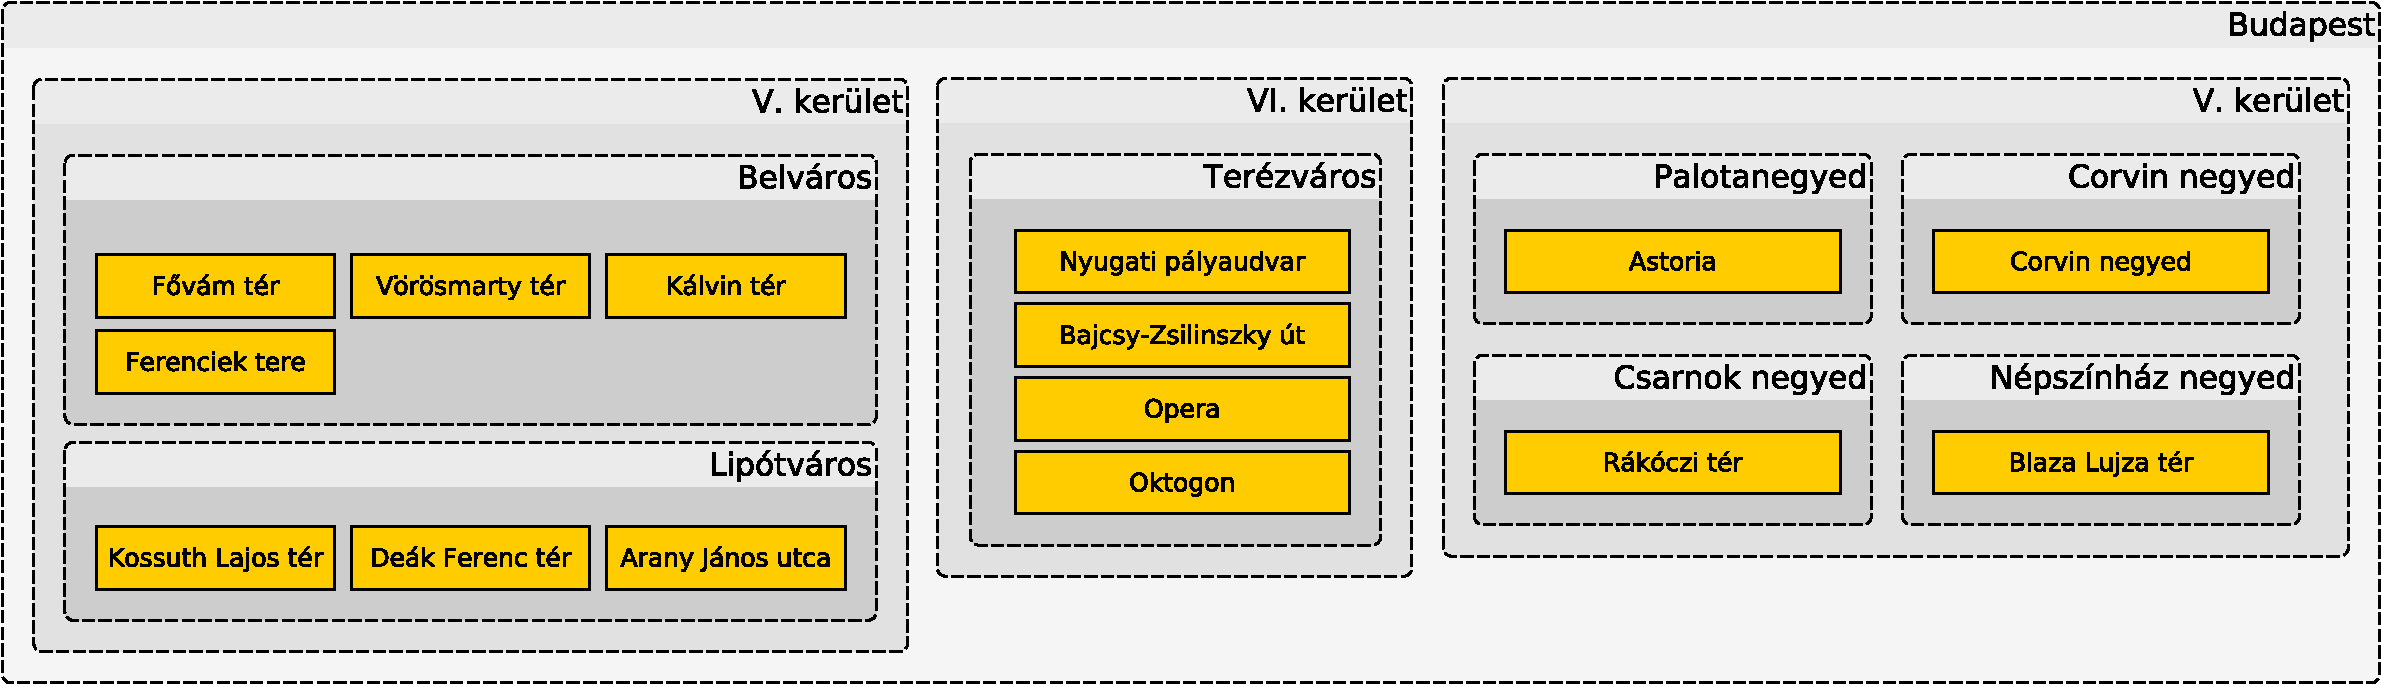
\includegraphics[scale=0.4]{implicit-tartalmazas}
		\caption{A tartalmazási viszonyok implicit módon jelölve}
		\label{fig:implicit-tartalmazas}
	\end{figure}
	
	\Aref{fig:implicit-tartalmazas}. ábrán egy olyan diagramot látunk, amelyben az egyes síkidomok közötti bennfoglaló ábrázolása reprezentálja a modellben szereplő tartalmazási viszonyt.
	
%	\added[id=szarnyas]{Ide be is tehetünk egy (kerületeket tartalmazó térképet), az jobb példa az explicit ábrázolásra}
\end{megjegyzes}

Láthattuk tehát, hogy mind a modellelemek közötti kapcsolat, mind a modellhierarchia hatékonyan ábrázolható gráfként. \Aref{fig:metrohalozat-hierarchiaval}. ábrán látható modell \aref{fig:metrohalozat-nagykorut-elcimkezett} és a \ref{fig:keruletek-varosreszek-metromegallok}. ábrákon található metróhálózatot és a területek hierarchiáját is tartalmazza.

\remofigscale{metrohalozat-hierarchiaval}{Budapest metróhálózata és a városrészek, kerületek hierarchiája}{\yedscale}

\subsection{Tulajdonságok}
\label{sec:tulajdonsagok}

\begin{pelda}
A közlekedési vállalat üzemen kívüli járművei telephelyeken parkolnak és itt végzik rajtuk a szükséges karbantartásokat. A metrók telephelyeinek neve metró \emph{járműtelep}, a buszoké az \emph{autóbuszgarázs}.

Mennyi üzemanyag raktározható a legnagyobb autóbusz garázsban? Milyen hosszú a Kőér utcai metró járműtelep vágányhálózata? Ezek a kérdések a modellünk elemeinek tulajdonságaival kapcsolatban merülnek fel. Építsünk modellt a problémára!
\end{pelda}

A telephelyeket például az alábbi modellel írhatjuk le:

\begin{table}[H]
	\centering
	\sf
\centering
\begin{tabular}{rllrrrr}
	\toprule
	\it azonosító & \it helyszín & \it funkció    & \it kapacitás & \it vágányhossz & \it max. üzemanyag &  \\ \midrule
	           T1 & Angyalföld   & kocsiszín      &           147 &          4922 m &                    &  \\
	           T2 & Budafok      & kocsiszín      &            46 &          2750 m &                    &  \\
	           T3 & Cinkota      & autóbuszgarázs &           265 &                 &      250~000 liter &  \\
	           T4 & Kelenföld    & kocsiszín      &            42 &          2829 m &                    &  \\
	           T5 & Kelenföld    & autóbuszgarázs &           322 &                 &      200~000 liter &  \\
	           T6 & Kelenföld    & metró járműterep &           x & yy                &       & \\
	           \bottomrule
\end{tabular}

% https://hu.wikipedia.org/wiki/Kelenf%C3%B6ldi_aut%C3%B3buszgar%C3%A1zs
% http://villamosok.hu/balazs/kcssz/budafok/index.html
% http://kozhir.blog.hu/2012/04/16/vendegsegben_metroeknal
% http://www.ancsingabor.hu/bkv_buszvezeto.html
	\caption{A BKK telephelyei (részleges modell)}
	\label{tab:jarmutelepek}
\end{table}

A modellünk elemei a táblázat sorai. A táblázat fejlécében definiált \fogalomragozva{tulajdonsag}{tulajdonságokból} (pl. helyszín, vágányhossz) az egyes modellelemek eltérő értékeket vehetnek fel. Látható, hogy a táblázatnak nem minden celláját töltöttük ki, mivel az egyes jellemzők nincsenek mindenhol értelmezve.

Megfigyelhetjük azonban, hogy az azonos %\fogalomragozva{tipus}{típussal}
funkcióval rendelkező modellelemek azonos tulajdonságokra vesznek fel értéket.
%Ez alapján megépíthetjük a problémához tartozó \fogalomragozva{tipushierarchia}{típushierarchiát}: minden \textsf{telephely} típusú elemre értelmezzük a helyszín és a kapacitás fogalmakat.
Mindkét típusú telephelynek van \textit{azonosító}, \textit{helyszín}, \textit{funkció} és \textit{kapacitás} attribútuma. Az \textsf{autóbuszgarázs} esetén a \textit{max. üzemanyag}, a \textsf{metró járműtelep} esetében a \textit{vágányhossz} attribútumot rögzítjük.

\subsection{Típusok}

\Aref{tab:jarmutelepek}. táblázat példájában láthattuk, hogy a \textit{funkció} jellemzővel megkülönböztethetjük az egyes a telephelyeket. Ha a \textit{funkció} jellemzőt a modellelemek \fogalomragozva{tipus}{típusának} tekintjük, akkor úgy is fogalmazhatunk, hogy a \textit{vágányhossz} jellemző csak a \textsf{metró járműtelep} típusú elemekre értelmezett, a \textit{max. üzemanyag} jellemző csak az \textsf{autóbuszgarázs} típusra. A típusokat felhasználhatjuk a gráfok jellemzésére is.

\begin{pelda}
	A korábbi metróhálózatot szeretnénk kiegészíteni a buszhálózatra vonatkozó információval. Szeretnénk tárolni azt is, hogy az egyes vonalakon közlekedő járművek melyik telephelyen parkolnak. Az autóbuszvonalon közelekedő járművek autóbuszgarázsban, a metróvonalon közlekedő járművek metró járműtelepen parkolnak.
\end{pelda}

Készítsünk egy példánygráfot, amelyen ábrázoljuk az M1 és M3-as metróvonal, valamint a 7-es és a 8-as buszvonalak kapcsolódásait (\textit{kapcsolódik) élek}, valamint azt, hogy az egyes vonalak melyik telephelyhez tartoznak (\textit{telephelye) élek}.

\remofigscalefixed{busz-metro-telephelyek}{Közlekedési vonalak és telephelyek}{\yedscale}

A példánygráfot követve a problémához tartozó típusgráfban meg kell jelennie a \textit{vonal} és a \textit{telephely} fogalmaknak. Az egyes vonalak kapcsolódhatnak egymáshoz a \textit{kapcsolódik} él mentén, míg a vonal telephelyét a \textit{telephelye} él jelzi.

\begin{megjegyzes}
Az egyes telephelyek tulajdonságait nem ábrázoltuk az ábrán.
\end{megjegyzes}

\remofigscalefixed{busz-metro-telephelyek-tipusgraf}{Közlekedési vonalak és telephelyek típusgráfja}{\yedscale}

A példánygráfot és a típusgráfot egy gráfban is jelölhetjük. Ekkor az egyes példányok és a típusok között egy \textit{példánya} él fut.

\remofigscalefixed{busz-metro-telephelyek-tipusgraffal}{Közlekedési vonalak és telephelyek példány- és típusgráfja}{\yedscale}

\Aref{fig:busz-metro-telephelyek-tipushierarchia}. ábra bemutatja a problémához tartozó \fogalomragozva{tipushierarchia}{típushierarchiát}. A típushierarchia egy hierarchikus modell, amely az egyes típusok leszármazási (\textit{is a}) viszonyait ábrázolja.

\remofigscalefixed{busz-metro-telephelyek-tipushierarchia}{Közlekedési vonalak és telephelyek típushierarchiája}{\yedscale}

A rendszer fejlesztésekor gyakran fontos, hogy a típusgráfot és a típushierarchiát együtt lássuk. A \fogalom{metamodell} tartalmazza a típusgráfot, a típusok hierarchiáját, a tulajdonságmodellt (ill. további, itt nem részletezett szabályokat, pl. multiplicitási kényszerek, jólformáltsági kényszerek).

A típusgráfban és a típushierarchiában tartalmazott információt, valamint tulajdonságmodellt együtt modellezve megkapjuk a terület metamodelljét. A metamodell részlete \aref{fig:busz-metro-telephelyek-metamodell}. ábrán látható.

\remofigscalefixed{busz-metro-telephelyek-metamodell}{Közlekedési vonalak és telephelyek (részleges) metamodellje}{\yedscale}

A példánymodellt és a metamodellt ábrázolhatjuk egyszerre is, a két modell elemei között a \emph{példánya} viszony teremt kapcsolatot (szürke szaggatott nyíl).

\remofigscalefixed{busz-metro-telephelyek-peldanymodell-metamodell}{Közlekedési vonalak és telephelyek példánymodellje és (részleges) metamodellje egy gráfon ábrázolva}{\yedscale}


\begin{feladat}
	Az egyes járműtelepek is valamelyik városrészhez tartoznak. Készítsünk olyan metamodellt, amelyben ábrázolható az egyes járműtelepek és városrészek kapcsolata is!
\end{feladat}



%Felismerhetjük, hogy a telephely helyszíne is belepasszol a városrészes gráfba. Ezzel sok fogalmat elég jól lehet szemléltetni: derived feature-ök, derived referenciák stb.

%\remofigscalefixed{jarmutelepek}{A közlekedési hálózatunk metamodellje}{\yedscale}


%TODO \fogalom{szarmaztatott-tulajdonsag}


%\begin{megjegyzes}
%A Zách utcai trolitelepen buszokat és trolikat is tárolnak. Alakítsuk át a modellt úgy, hogy ezt is tudja modellezni. % http://www.bkk.hu/2013/09/villamosnap-budafokon-es-nyilt-nap-a-trolitelepen/
%\end{megjegyzes}

%\begin{pelda}
%	Melyik a legnagyobb teljesítményű jármű? Milyen jellemzőket kell rögzíteni egy újonnan beszerzett buszról? Ezek a kérdések a modellünk elemeinek tulajdonságaival kapcsolatban merülnek fel.
%\end{pelda}
%
%Készítsünk egy modellt, ami a különböző járműveket tartalmazza. Ezt a modellt gráf helyett inkább táblázatos formában érdemes ábrázolni, így jobban áttekinthető lesz.
%
%\begin{table}[H]
%	\centering
%	\begin{tabular}{|l|l|l|l|l|r|l|l|}
%		\hline
%		név                   & típus    & tömeg & hossz & lökettérfogat & \#motorok & telj. & nyomtáv \\ \hline\hline
%		Volvo 7700            & busz     & 18 t  & 12 m  & 9000 cm$^3$   &               & 320 LE       &         \\ \hline
%		Siemens Combino Supra & villamos & 70 t  & 54 m  &               & 8             & 800 kW       & 1800 mm \\ \hline
%		XY & villamos & a t  & b m  &               & 8             & yy kW       & 1800 mm \\ \hline
%		Alstom Metropolis     & metró    &       &       &               &               &              & 1435 mm \\ \hline
%	\end{tabular}
%	\caption{Járművek tulajdonságai}
%	\label{tab:jarmuvek}
%\end{table}
%
%A modellünk elemei itt a táblázat sorai. A modellelemek tulajdonságait \fogalomragozva{jellemzo}{jellemzőkkel} vagy más néven \fogalomragozva{attributum}{attribútumokkal} írjuk le. Mint \aref{tab:jarmuvek}. táblázatban látható, különböző modellelemekre az egyes jellemzők más-más értéket vehetnek fel. Látható, hogy a táblázatnak nem minden celláját töltöttük ki, mivel az egyes jellemzők nincsenek mindenhol értelmezve. Ezeket a cellákat gyakran az \rovidites{NA} (\roviditesangolul{NA}) rövidítéssel vagy \textsf{null} értékkel jellemezzük. Megfigyelhetjük azonban, hogy az azonos \fogalomragozva{tipus}{típussal} rendelkező modellelemek azonos tulajdonságokra vesznek fel értéket.

%A jellemzők nem is feltétlenül értelmezettek minden modellelemre (ún. \fogalomragozva{parcialis-fuggveny}{parciális függvényként} írhatóak le a matematika nyelvén).


%%%%%%%%%%%%%%%%%%%%%%%%%%%%%%%%%%%%%%%%%%%%%%%%%%%%%%%%%%%%%%%%%%%%%%%%%%%%%%%%

\section{A struktúramodellezés elmélete}

%Ahogy \az+\refstruc{sec:motivacio} 

Ahogy az eddigi példákban láttuk, a struktúramodellezés célja, hogy a rendszer felépítését jellemezze, beleértve az egyes elemek típusát, a közöttük lévő kapcsolatokat és hierarchiát, valamint az elemek tulajdonságait. Egy rendszer strukturális modellje tehát alkalmas arra, hogy az alábbi kérdésekre (nem feltétlenül kimerítő) választ nyújtson:

\begin{itemize}
	\item Milyen elemekből áll a rendszer?
	\item Hogyan kapcsolódnak egymáshoz az elemek?
	\item Milyen hierarchia szerint épül fel a rendszer?
	\item Milyen tulajdonságúak a rendszer elemei?
\end{itemize}

%A strukturális modell elkészítéséhez jellemeznünk kell a rendszerünk elemeinek aspektusait: a típusukat, az elemek közötti hierarchiát és kapcsolatokat, valamint az elemek jellemzőit.

A strukturális modellre az alábbi tömör definíciót adhatjuk.

\begin{definicio}
	A \fogalom{strukturalis-modell} a rendszer felépítésére (\fogalomragozva{struktura}{struktúrájára}) vonatkozó tudás. A strukturális modell a rendszer alkotórészeire, ezek tulajdonságaira és egymással való viszonyaira vonatkozó statikus (tehát változást nem leíró) tudást reprezentál. %Az egyes modellelemek \fogalomragozva{egyedi}{egyediek}.
\end{definicio}

%A strukturális modell aspektusa: fizikai (felépítés), logikai (funkció)

A következőkben a korábbi példákra építve bemutatjuk a struktúramodellezés elméleti hátterét és precízen definiáljuk a szükséges fogalmakat.

\subsection{Tulajdonságmodell}

\begin{definicio}
	A \fogalom{jellemzo} egy, a modell által megadott \fogalom{parcialis-fuggveny}, amelyet a modellelemeken értelmezünk.
\end{definicio}

\begin{megjegyzes}
	A $H$ halmazon értelmezett \fogalom{parcialis-fuggveny} nem jelent mást, mint a $H$ valamely (nem megnevezett) részhalmazán értelmezett \fogalom{fuggveny}. Konkrét esetünkben az egyes jellemzőket a modellelemek egy-egy részére értelmezzük (nem feltétlenül az összesre).
\end{megjegyzes}

A jellemzőket gyakran táblázatos formában ábrázoljuk. Vizsgáljuk meg például \aref{tab:jarmutelepek}. táblázat jellemzőit:

\begin{table}[H]
	\centering
	\sf
\centering
\begin{tabular}{rllrrrr}
	\toprule
	\it azonosító & \it helyszín & \it funkció    & \it kapacitás & \it vágányhossz & \it max. üzemanyag &  \\ \midrule
	           T1 & Angyalföld   & kocsiszín      &           147 &          4922 m &                    &  \\
	           T2 & Budafok      & kocsiszín      &            46 &          2750 m &                    &  \\
	           T3 & Cinkota      & autóbuszgarázs &           265 &                 &      250~000 liter &  \\
	           T4 & Kelenföld    & kocsiszín      &            42 &          2829 m &                    &  \\
	           T5 & Kelenföld    & autóbuszgarázs &           322 &                 &      200~000 liter &  \\
	           T6 & Kelenföld    & metró járműterep &           x & yy                &       & \\
	           \bottomrule
\end{tabular}

% https://hu.wikipedia.org/wiki/Kelenf%C3%B6ldi_aut%C3%B3buszgar%C3%A1zs
% http://villamosok.hu/balazs/kcssz/budafok/index.html
% http://kozhir.blog.hu/2012/04/16/vendegsegben_metroeknal
% http://www.ancsingabor.hu/bkv_buszvezeto.html
\end{table}


\begin{megjegyzes}
	A tulajdonságmodell mögötti matematikai struktúra az ún. \fogalomragozva{relacio}{reláció}. A reláció pontos halmazelméleti definíciójával és a relációkon értelmezett műveleteket definiáló \fogalomragozva{relacioalgebra}{relációalgebrával} bővebben az \adatb tárgy foglalkozik.
\end{megjegyzes}

A modellelemeket az \textit{azonosító} jellemzőjükkel különböztetjük meg egymástól. % rendelkeznek \fogalomragozva{egyedi-azonosito}{egyedi azonosítóval}.
A \textit{kapacitás} jellemzőhöz tartozó függvény
$\mathit{kapacitás}(e) \rightarrow n,$
ahol $e$ egy modellelem azonosítója, $n$ egy nemnegatív egész szám. 
Például
$$\mathit{kapacitás}(\mathsf{T2}) = 60, \quad \mathit{kapacitás}(\mathsf{T3}) = 265.$$

A \textit{funkció} jellemzőhöz tartozó függvény
$\mathit{funkció}(e) \rightarrow t,$
ahol $e$ egy modellelem azonosítója, $t$ a $\{\textsf{metró járműtelep}, \textsf{autóbuszgarázs}\}$ halmaz eleme.
Például
$$\mathit{funkció}(\mathsf{T2}) = \textsf{metró járműtelep}, \quad \mathit{funkció}(\mathsf{T3}) = \textsf{autóbuszgarázs}.$$

A fentiekhez hasonlóan, a \textit{vagányhossz} jellemzőhöz tartozó parciális függvény 
$\mathit{vagányhossz}(e) \rightarrow n,$
ahol $e$ egy modellelem azonosítója, $n$ egy nemnegatív egész szám. Fontos különbség viszont az eddigiekhez képest, hogy ezt jellemzőt csak bizonyos modellelemekre értelmeztünk, másokra nem: a metró járműtelepek esetén vesz fel értéket, az autóbuszgarázsok esetén viszont nem. Vagyis látható, hogy a \textit{vagányhossz} jellemző csak akkor vesz fel értéket, ha a \textit{funkció} attribútum értéke \textsf{metró járműtelep}.

Ha tehát a \textit{funkció} attribútumot a telephely \fogalomragozva{tipus}{típusának} tekintjük, akkor úgy is fogalmazhatunk, hogy a \textit{vágányhossz} jellemző csak a \textsf{metró járműtelep} típusú elemekre értelmezett. Általánosan:

\begin{definicio}	
	A \fogalom{tipus} egy kitüntetett jellemző, amely meghatározza, hogy milyen más jellemzők lehetnek értelmezettek az adott modellelemre, illetve milyen más modellelemekkel lehet kapcsolatban. A többi jellemzőt \fogalomragozva{tulajdonsag}{tulajdonságnak} hívjuk.

\begin{megjegyzes}
	Jelen anyagban az egyszerűség kedvéért feltételezzük, hogy a modellelemeknek pontosan egy típusa van.
\end{megjegyzes}
\end{definicio}


A modellünkben két típus van: az \textsf{autóbuszgarázs} és a \textsf{járműtelep}. Például a cinkotai telephely az \textsf{autóbuszgarázs}, míg a mexikói úti telephely a \textsf{metró járműtelep} típus példánya.

\begin{definicio}
Egy adott $t$ típus \fogalomragozva{peldany}{példányainak} nevezzük azon modellelemeket, amelyek típusa $t$.
\end{definicio}

A modellezési gyakorlatban elterjedt (de nem univerzális) megkötés, hogy az egyes elemek típusát állandónak tekintjük. Ha az elem típusa a rendszer működése során nem változhat meg, akkor olyan típust kell hozzárendelni, amely az elem teljes életciklusa során előforduló összes lehetséges jellemzővel, kapcsolattal összhangban van.

\subsection{Gráfmodellek}

\begin{kisdefiniciok}
	A definíciók támaszkodnak a gráfelmélet alapjaira, ezért röviden összefoglaljuk a felhasznált definíciókat.
	
	A \fogalom{graf} egy olyan $G = (V, E)$ struktúra, ahol $V$ halmaz a csomópontok, $E$ az élek halmaza. Az élek csomópontok között futnak, \fogalom{iranyitatlan-graf} esetén az $E$ halmaz csomópontok rendezetlen $\{v_1, v_2\}$ párjaiból áll (tehát nem különböztetjük meg a $\{v_1, v_2\}$ és a $\{v_2, v_1\}$) párokat, míg \fogalom{iranyitott-graf} esetén csomópontok rendezett $(v_1, v_2)$ párjaiból.
	% Egy gráf \fogalomragozva{egyszeru-graf}{egyszerű}, ha nem tartalmaz többszörös és hurokélet.
	
	\fogalomragozva{cimkezett-graf}{Címkézett gráf} esetén a gráf elemeit (csomópontjait és/vagy éleit) \fogalomragozva{cimke}{címkékkel} láthatjuk el. A címkézés célja lehet \fogalom{egyedi-azonosito} hozzárendelése vagy bizonyos tulajdonság leírása (pl. a csomópontok kapacitása, élek típusa). Ha precízen szeretnénk jellemezni a gráfot, a következő terminológiát használhatjuk: ha csak a csomópontokhoz rendelünk címkéket, \fogalomragozva{csucscimkezett-graf}{csúcscímkézett} gráfról beszélünk, míg ha csak a gráf éleihez rendelünk címkéket, \fogalomragozva{elcimkezett-graf}{élcímkézett} gráfról beszélünk. 
	
	%A \fogalom{sulyozott-graf} olyan $(G, w)$ pár, ahol $G = (V, E)$ gráf, $w: E \rightarrow \mathbb{R}$ egy súlyfüggvény.
\end{kisdefiniciok}

A típusok gráf jellegű modellek esetén is fontos szerepet játszanak. A gráfmodell elemeit (külön-külön a csomópontokat és az éleket is) típusokba sorolhatjuk. A típusok meghatározzák, hogy az egyes csomópontok milyen élekkel köthetők össze.

Az egyes csomópont- és éltípusok viszonyát gráfként is ábrázolhatjuk.

\begin{definicio}
	A \fogalom{tipusgraf} egy olyan gráf, amelyben minden csomóponttípushoz egy típuscsomópont, minden éltípushoz egy típusél tartozik.
\end{definicio}

A gráfmodelleken is értelmezzük a \fogalom{peldany} fogalmát.

\begin{definicio}
	Egy adott típusgráf \fogalomragozva{peldanygraf}{példánygráfja} alatt olyan gráfmodellt értünk, amelynek elemei a típusgráf csomópont- és éltípusainak példányai, valamint minden él forrása és célja rendre az éltípus forrásának és céljának példánya.
\end{definicio}

A típusgráfot és példánygráfot egy gráfon ábrázolva a típus-példány viszonyok is megjeleníthetők: a példánygráf csomópontjaiból a típusgráf csomópontjaira \fogalomangolul{peldanya} (\fogalom{peldanya}) élek mutatnak. Szintén \fogalomangolul{peldanya} viszony áll fenn a példánygráf élei és a típusgráf élei között.% -- ennek ábrázolása azonban gráfként nehézkes.

\begin{megjegyzes}
	Az \fogalomangolul{peldanya} viszony helyett gyakran annak inverzét, a \fogalomangolul{tipusa} (x \fogalom{tipusa} y-nak) viszonyt. Gráfban ábrázolva az \fogalom{peldanya} és \fogalom{tipusa} élek adott csomópontok között egymással ellentétes irányúak.
\end{megjegyzes}

\remofigscalefixed{busz-metro-telephelyek-tipusgraf-inverz-elek}{Példány és típusgráf \fogalomangolul{tipusa} élekkel}{\yedscale}

\begin{definicio}
	Egy rendszer \fogalomragozva{metamodell}{metamodellje} tartalmazza a típusgráfot, az egyes típusok közötti kapcsolatokat, ill. további megkötéseket is.
	
	\begin{megjegyzes}
		A további megkötések között szerepelhet az egyes tulajdonságok láthatósága, az egyes modellelemeken értelmezett művelete, multiplicitási kényszerek stb. Ezekkel most nem foglalkozunk részletesen.
	\end{megjegyzes}
\end{definicio}

\subsection{Hierarchia}

\begin{kisdefiniciok}
	A \fogalom{seta} szomszédos csúcsok és élek váltakozó sorozata, mely csúccsal kezdődik és csúcsban végződik. %Ha egy séta során egy gráfelemet sem érintünk többször, útról beszélünk, tehát
	Az \fogalom{ut} olyan séta, amely nem metszi önmagát, valamint első és utolsó csúcsa különbözik. A \fogalom{kor} olyan séta, amely nem metszi önmagát, valamint első és utolsó csúcsa megegyezik. %Körről beszélünk, ha egy út során ugyanoda érünk vissza, ahonnan elindultunk.	
	%Ezek ismeretében már beszélhetünk körmentes gráfokról.
	A körmentes, összefüggő gráfokat \fogalomragozva{fa-graf}{fának} nevezzük. (A körmentes gráfokat \fogalomragozva{erdo}{erdőnek} nevezzük.)
	A fák esetén gyakran kiemelt szerepet tulajdonítunk egy csomópontnak: a \fogalom{gyoker-csomopont} a fa egy megkülönböztetett csomópontja. A \fogalom{gyokeres-fa} olyan fa, ami rendelkezik gyökér csomóponttal. \Fogalom{gyokeres-szintezett-fa} esetén a fa csomópontjaihoz hozzárendeljük a gyökértől vett távolságukat is.
	
	A hierarchikus modellezésben kiemelt szerepet játszanak az irányított körmentes gráfok. Egy gráf \rovidites{DAG} (\roviditesangolul{DAG}), ha nem tartalmaz irányított kört.	
\end{kisdefiniciok}

Egy rendszer hierarchiája a rendszer dekompozíciójával állítható elő.

\begin{definicio}
	A \fogalom{dekompozicio} (\fogalom{faktoring}) egy rendszer kisebb \fogalomragozva{komponens}{komponensekre} bontása, amelyek könnyebben érthetők, fejleszthetők és karbantarthatók.
\end{definicio}

A rendszer így kapott egyes komponensei (részrendszerei) gyakran további dekompozícióval még kisebb részekre bonthatóak. Természetesen a dekompozíció során ügyelnünk kell arra, hogy az egyes részekből visszaállítható legyen az eredeti rendszer, különben a kapott strukturális modellünk hiányos.

\begin{definicio}
	Egy dekompozíció \fogalomragozva{helyes-dekompozicio}{helyes}, ha a dekompozícióval kapott rendszer minden elemének megfeleltethető az eredeti rendszer valamelyik eleme, és az eredeti rendszer minden eleméhez hozzárendelhető a dekompozícióval kapott rendszer egy vagy több eleme.
\end{definicio}


%Korábban láttuk, hogy a hierarchiában nincs kör és ezt egyébként fának nevezzük. Ha irányított a gráf, akkor az a fontos, hogy irányított kör ne legyen benne.

%A hierarchiát reprezentáló modellek körmentes gráfot alkotnak, szigorú hierarchia esetén ez \fogalomragozva{fa-graf}{fa} vagy \fogalom{erdo}, megengedő hierarchia esetén \rovidites{DAG}.










%%%%%%%%%%%%%%%%%%%%%%%%%%%%%%%%%%%%%%%%%%%%%%%%%%%%%%%%%%%%%%%%%%%%%%%%%%%%%%%%%%%%%%%%%%%%%%%%%%%%



\section{Nézetek}

A struktúramodellekből különböző \fogalomragozva{nezet}{nézeteket} állíthatunk elő. 

Tulajdonságmodelleken a leggyakrabban használt műveletek a \fogalom{szures} és a \fogalom{vetites}. Ezek során úgy \fogalomragozva{absztrakcio}{absztraháljuk} a modellt, hogy bizonyos modellelemeket és/vagy azok egyes jellemzőit elhagyjuk.

\begin{megjegyzes}
	A relációalgebrában a \fogalom{szures} művelet neve \fogalom{szelekcio}, a \fogalom{vetites} művelet neve \fogalom{projekcio}.
\end{megjegyzes}

\subsection{Szűrt nézet}

Ismét idézzük fel \az+\refstruc{tab:jarmutelepek} telephelyeket tartalmazó tulajdonságmodelljét.

\begin{table}[H]
	\centering
	\sf
\centering
\begin{tabular}{rllrrrr}
	\toprule
	\it azonosító & \it helyszín & \it funkció    & \it kapacitás & \it vágányhossz & \it max. üzemanyag &  \\ \midrule
	           T1 & Angyalföld   & kocsiszín      &           147 &          4922 m &                    &  \\
	           T2 & Budafok      & kocsiszín      &            46 &          2750 m &                    &  \\
	           T3 & Cinkota      & autóbuszgarázs &           265 &                 &      250~000 liter &  \\
	           T4 & Kelenföld    & kocsiszín      &            42 &          2829 m &                    &  \\
	           T5 & Kelenföld    & autóbuszgarázs &           322 &                 &      200~000 liter &  \\
	           T6 & Kelenföld    & metró járműterep &           x & yy                &       & \\
	           \bottomrule
\end{tabular}

% https://hu.wikipedia.org/wiki/Kelenf%C3%B6ldi_aut%C3%B3buszgar%C3%A1zs
% http://villamosok.hu/balazs/kcssz/budafok/index.html
% http://kozhir.blog.hu/2012/04/16/vendegsegben_metroeknal
% http://www.ancsingabor.hu/bkv_buszvezeto.html
\end{table}

\begin{definicio}
	A \fogalomragozva{szures}{szűrés} művelet során a modell elemein kiértékelünk egy szűrési feltételt és azokat tartjuk meg, amelyek megfelelnek a feltételnek.
\end{definicio}

Tulajdonságmodellek esetén a szűrés az elhagyott modellelemek a modell sorai lehetnek, gráf jellegű modellek esetén a gráf csúcsai vagy élei.

\subsubsection{Tulajdonságmodell szűrése}

\begin{pelda}
	Szeretnénk megtudni, hogy mely telephely alkalmas legalább 100 jármű befogására.
\end{pelda}

Azokra az elemekre szűrünk, amelyeknél a \textsf{kapacitás} jellemző értéke 100-nál nagyobb vagy egyenlő.
%$$\sigma_{\mathsf{kapacitás} \,\geq\, 100} (\textsf{telephely})$$

Az eredmény:
\begin{table}[H]
	\centering
	\sf
	\centering
	\begin{tabular}{rllrrrr}
		\toprule
		\it azonosító & \it helyszín & \it funkció      & \it kapacitás & \it vágányhossz & \it max. üzemanyag &  \\ \midrule
		T3 & Cinkota      & autóbuszgarázs   &           265 &                 &      250~000 liter &  \\
		T4 & Kelenföld    & autóbuszgarázs   &           322 &                 &      200~000 liter &  \\ 
		\bottomrule
	\end{tabular}
\end{table}
	
\begin{pelda}
	Szeretnénk megtudni, hogy mely metró járműtelep alkalmas legalább 50 jármű befogására.
\end{pelda}

Végezzünk szűrést azokra a modellelemekre, ahol a \textit{funkció} attribútum értéke \textsf{metró járműtelep}, a \textit{kapacitás} attribútum értéke nagyobb vagy egyenlő 50-nél.

Az eredmény:
\begin{table}[H]
	\sf
	\centering
	\begin{tabular}{rllrrrr}
		\toprule
		\it azonosító & \it helyszín & \it funkció      & \it kapacitás & \it vágányhossz & \it max. üzemanyag &  \\ \midrule
		T2 & Kőér utcai   & metró járműtelep &            60 &        16~512 m &                    &  \\
		\bottomrule
	\end{tabular}
\end{table}

\subsubsection{Gráfmodell szűrése}

Egy gráfmodellből a szűrés a modell egy \fogalomragozva{reszgraf}{részgráfját} állítja elő.

\begin{pelda}
	Soroljuk fel az M2-es és az M4-es metró megállóit.
\end{pelda}

A modellen szűrést végzünk, ami csak azokat a csomópontokat tartja meg, amelyekhez tartozik olyan él, amelynek a címkéje M2 vagy M4. A kapott részgráf \aref{fig:metrohalozat-nagykorut-elcimkezett-szurt} ábrán látható.

\begin{pelda}
	Határozzuk meg, hogy mely szomszédos metrómegállók között hosszabb egy percnél a menetidő.	
\end{pelda}

A modellen szűrést végzünk, ami

\begin{itemize}
	\item csak azokat a csomópontokat tartja meg, amelyekhez tartozik 1-nél nagyobb súlyú él,
	\item csak az 1-nél nagyobb súlyú éleket tartja meg.
\end{itemize}

A kapott részgráf \aref{fig:metrohalozat-nagykorut-elsulyozott-szurt} ábrán látható.

\begin{figure}[H]
	\begin{subfigure}[b]{0.5\textwidth}
		\centering
		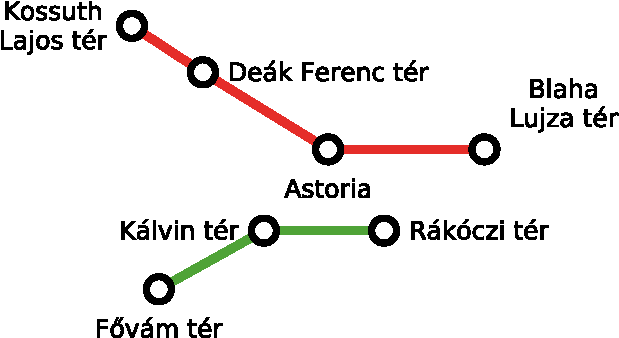
\includegraphics[scale=\yedscale]{metrohalozat-nagykorut-elcimkezett-szurt}
		\caption{Az M2 és az M4 metróvonalak megállói}
		\label{fig:metrohalozat-nagykorut-elcimkezett-szurt}
	\end{subfigure}
	~
	\begin{subfigure}[b]{0.5\textwidth}
		\centering
		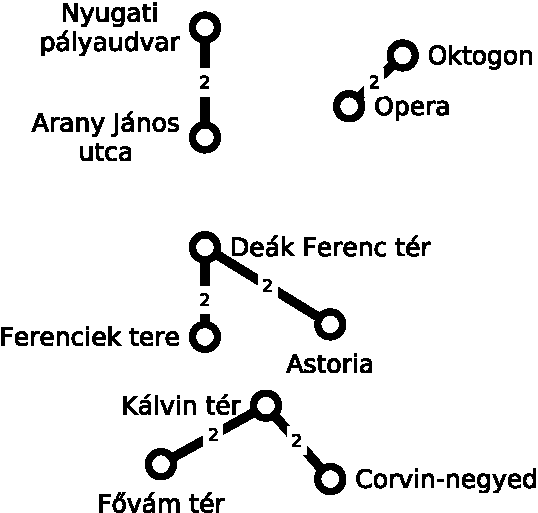
\includegraphics[scale=\yedscale]{metrohalozat-nagykorut-elsulyozott-szurt}
		\caption{Az 1 percnél távolabbi metrómegállók}
		\label{fig:metrohalozat-nagykorut-elsulyozott-szurt}
	\end{subfigure}
	\caption{Szűrések a metróhálózatot tartalmazó gráfon}
\end{figure}


\subsection{Vetített nézet}

\begin{definicio}
	\Fogalom{vetites} során a modell egyes jellemzőit kiválasztjuk és a többit elhagyjuk a relációból.

\begin{megjegyzes}
	Érvényes vetítés művelet az is, ha a tulajdonságmodell összes jellemzőjét megtartjuk.
\end{megjegyzes}
\end{definicio}

\subsubsection{Tulajdonságmodell vetítése}

\begin{pelda}
	Olyan kimutatásra van szükségünk, ami csak az egyes telephelyek helyszínét, funkcióját és kapacitását tartalmazza.
%	$$\pi_{\textsf{helyszín, kapacitás}} (\textsf{telephely})$$
\end{pelda}

Végezzünk szűrést a tulajdonságmodelleken a \textit{helyszín}, \textit{funkció} és a \textit{kapacitás} attribútumokra.

\begin{table}[H]
	\sf
	\centering
	\begin{tabular}{llr}
		\toprule
		\it helyszín & \it funkció      & \it kapacitás \\ \midrule
		Mexikói út   & metró járműtelep &            24 \\
		Kőér utcai   & metró járműtelep &            60 \\
		Cinkota      & autóbuszgarázs   &           265 \\
		Kelenföld    & autóbuszgarázs   &           322 \\ \bottomrule
	\end{tabular}
\end{table}

\subsubsection{Gráfmodell vetítése}

A tulajdonságmodellhez hasonlóan a gráfmodellből is elhagyhatunk jellemzőket.

\begin{pelda}
	\ldots
\end{pelda}

\ldots

%%%%%%%%%%%%%%%%%%%%%%%%%%%%%%%%%%%%%%%%%%%%%%%%%%%%%%%%%%%%%%%%%%%%%%%%%%%%%%%%%%%%%%%%%%%%%%%%%%%%

\section{Struktúramodellezési technikák}

%Fontos gondolat: a struktúramodellezésnek többféle célja lehet.
%
%
%\begin{itemize}
%	\item Készítsünk egy adatmodellt a rendszerünkhöz, pl. egy pizzarendelő oldalon elkészítjük az adatbázis modelljét. Ezután az adatbázis a felhasználói interakcióknak megfelelően változik. Ez a modell ,,típusgráf'' része.
%	
%	\item Készítsünk a problémából egy modellt, amiből bizonyos kérdésekre választ kaphatunk. Például az alaprajzával modellezzünk egy épületet és nézzük meg, hogy bizonyos tűzvédelmi szempontoknak megfelel-e. Ez a modell ,,példánygráf'' része.
%\end{itemize}

A modellezési formalizmusok után bemutatunk néhány struktúramodellezési technikát.

\subsection{Hierarchia modellezése}

Korábban láttuk, hogy a modellelemek közti szigorú hierarchia kifejezhető fa (ill. erdő) gráfokkal. Ezek a fajta modellek képesek kifejezni a (rész)rendszerek és alkotóelemeik közti tartalmazási viszonyt, akár többlépcsős tartalmazással is (a részrendszerek is további részeket tartalmaznak). Azonban a gyakorlatban a modellnek sokszor ennél jóval több információt kell tartalmaznia; egy-egy adott modellelemmel kapcsolatban nem csak a tartalmazó és tartalmazott komponenseivel való tartalmazási viszonyát kell ismerni, hanem egyéb modellelemekkel való kapcsolatait. Ilyenkor a strukturális modell (gráf jellegű része) két rétegre tagozódik: egyrészt a modell szerkezeti vázát alkotó tartalmazási hierarchiára (fa/erdő), amely az alkotóelemek rész-egész viszonyait reprezentálja, másrészt ezen felüli \fogalom{kereszthivatkozas} élekre, amelyek a tartalmazási rendtől függetlenül, a körmentesség korlátozása nélkül köthetnek össze elemeket. Ennek megfelelően egy metamodell megmondhatja, hogy mely éltípusok példányait fogjuk az említett szerkezeti vázat alkotó tartalmazási éleknek tekinteni. 

A hierarchikus modellek megalkotása, illetve az összetett rendszerek tervezése során többféleképp választható meg az egyes elemek elkészítésének sorrendje. Jól illusztrálja a választási szabadságot két polárisan ellentétes megközelítés: a \fogalomangolul{top-down} és a \fogalomangolul{bottom-up} modellezés.

\begin{definicio}
	\Fogalomangolul{top-down} modellezés során a rendszert felülről lefelé (összetett rendszerből az alkotóelemei felé haladva) építjük. A modellezés alaplépése a \fogalom{dekompozicio}.
\end{definicio}

Egy top-down modellezési / tervezési folyamatot úgy kell tehát elképzelni, hogy a kezdetektől fogva az egész rendszer modelljét építjük; azonban eleinte hiányoznak még a részletek. Idővel a modellt finomítjuk: tartalmazott alkotóelemekre bontjuk a rendszert, megadva azok tulajdonságait és kereszthivatkozásait is; majd később magukat az alkotóelemeket ugyanúgy strukturális dekompozíciónak vetjük alá. 

A top-down modellezés fontos jellemzői:

\begin{itemize}
	\item[$\oplus$] Részrendszer tervezésekor a szerepe már ismert
	\item[$\ominus$] ,,Félidőben'' még nincsenek működő (teljes részletességgel elkészített) részek
	\item[$\ominus$] Részek problémái, igényei későn derülnek ki
\end{itemize}

\begin{definicio}
	\Fogalomangolul{bottom-up} modellezés során a rendszert alulról felfelé (elszigetelt alkotóelemekből az összetett rendszer felé haladva) építjük. A modellezés alaplépése a \fogalom{kompozicio}: az egész rendszer összeszerkesztése külön modellezett vagy fejlesztett részrendszerekből.
\end{definicio}

Egy bottom-up modellezési / tervezési folyamatot úgy kell tehát elképzelni, hogy a kezdetektől fogva részletes modelleket építünk; azonban eleinte csak a rendszer izolált, egyszerű komponenseivel foglalkozunk. Ahogy fokozatosan egyre több komponens készül el, nagyobb részrendszerekké foglalhatjuk őket össze, az egymáshoz való kapcsolódásukat is tisztázva. Idővel az így kapott összetettebb részrendszereket is további kompozíciónak vethetjük alá. 

A bottom-up modellezés fontos jellemzői:

\begin{itemize}
	\item[$\oplus$] A rendszer részei önmagukban kipróbálhatók, tesztelhetők
	\item[$\oplus$] Részleges készültségnél könnyebben előállítható a rendszer prototípusa
	\item[$\ominus$] Nem látszik előre a rész szerepe az egészben
\end{itemize}

Természetesen a gyakorlatban a kétféle szélsőséges megközelítés közti kompromisszum is elképzelhető.

%\subsection{Metamodellezés}
%
%Egy adott problématerület metamodelljét gyakran informatikai szakemberek készítik, az adott terület szakértőivel -- ún. \emph{domain expertök} -- együttműködve.
%
%Ontológia készítése, ...
%
%\subsubsection{Taxonómia és ontológia}
%
%\begin{definicio}
%	A \fogalom{taxonomia} ...
%\end{definicio}
%
%Az ontológia kifejezésre sok különböző definíció létezik. Az informatikában általában az alábbihoz hasonló módon definiálják:
%
%\begin{definicio}
%	Az \fogalom{ontologia} egy olyan \fogalom{taxonomia}, amely tartalmazza a benne szereplő fogalmak közötti viszonyokat. 
%\end{definicio}
%
%\todo{RDF}


%%%%%%%%%%%%%%%%%%%%%%%%%%%%%%%%%%%%%%%%%%%%%%%%%%%%%%%%%%%%%%%%%%%%%%%%%%%%%%%%%%%%%%%%%%%%%%%%%%%%
%
%
%\section{Az objektum-orientált modell}
%
%\Fogalom{objektum-orientalt} modellezés során a világot úgy modellezzük, hogy a modellünk elemei \fogalomragozva{objektum}{objektumok}, amelyek \fogalomragozva{attributum}{attribútumokkal} rendelkeznek egymással különböző kapcsolatokat (\fogalomragozva{asszociacio}{asszociációk}) vehetnek fel. Az objektumok típusát az \fogalomragozva{osztaly}{osztályuk} határozza meg.
%
%Az objektum-orientált modell ereje abban rejlik, hogy képes a típusok, a hierarchia, a kapcsolatok és az attribútumok precíz ábrázolására.
%
%TODO: \fogalom{orokles}, \fogalom{alosztaly}, \fogalom{ososztaly}
%
%\begin{megjegyzes}
%	Az \roviditesmagyarul{OOP} (\rovidites{OOP}) foglalkozik az egyes osztályokon végzett műveletekkel \fogalomragozva{metodus}{metódusaival}, ill. az egyes metódusok és \fogalomragozva{mezo}{mezők} láthatóságával is.
%	
%	A \fogalom{tobbszoros-orokles} több felveti a \fogalom{gyemant-problema}
%	
%	Ezekről bővebben a \progketto, a \progharom és a \szofttech tárgyakban esik szó.	
%\end{megjegyzes}
%
%
%
%
%Többszintű metamodellezés: járműtípus, járműpéldány modellezése; 
%
%%%%%%%%%%%%%%%%%%%%%%%%%%%%%%%%%%%%%%%%%%%%%%%%%%%%%%%%%%%%%%%%%%%%%%%%%%%%%%%%%%%%%%%%%%%%%%%%%%%%

\section{Gyakorlati alkalmazások}

\subsection{Számítógéphálózat modellezése}

Számítógép-hálózatok kiválóan modellezhetők gráfokkal, amelyben a gráf csomópontjai a hálózat elemei (pl. számítógép, router, tűzfal), a kapcsolatok pedig ezek összeköttetései.

\remofigscalefixed{halozat}{Hálózat}{0.35}

\begin{itemize}
	\item Milyen elemekből áll a rendszer, milyen kapcsolatok lehetségesek?
	\item Van-e egyszeres hibapont a rendszerben?
	\item Milyen hosszú úton, milyen típusú elemeket érintve lehet elérni az internetet?
	\item Hány gép van a wifi hálózaton?
	\item Egy elem hibája meddig terjedhet?
	\item Elérhető-e az internet?
\end{itemize}

\begin{feladat}
	Milyen típushierarchiát készíthetünk egy számítógép-hálózathoz?
\end{feladat}

\subsection{Grafikus felhasználói felület}

Egy szoftver alkalmazás \emph{\glslink{GUI}{grafikus felhasználói felülete}} (\glslink{GUI}{GUI}) is egy hierarchikus modell.

\begin{figure}[H]
	\begin{subfigure}[b]{0.5\textwidth}
		\centering
		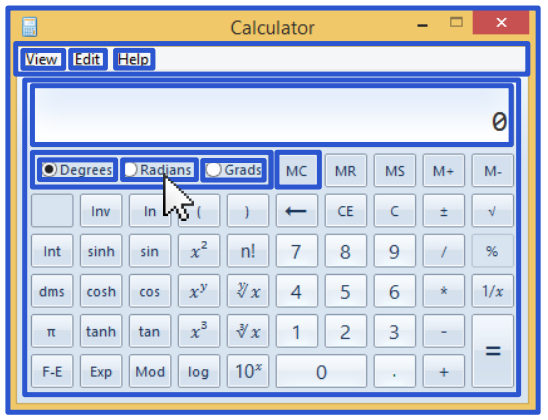
\includegraphics[scale=0.4]{GUI-ablak}
		\caption{A számológép alkalmazás grafikus felülete}
		\label{fig:GUI-ablak}
	\end{subfigure}
	~
	\begin{subfigure}[b]{0.5\textwidth}
		\centering
		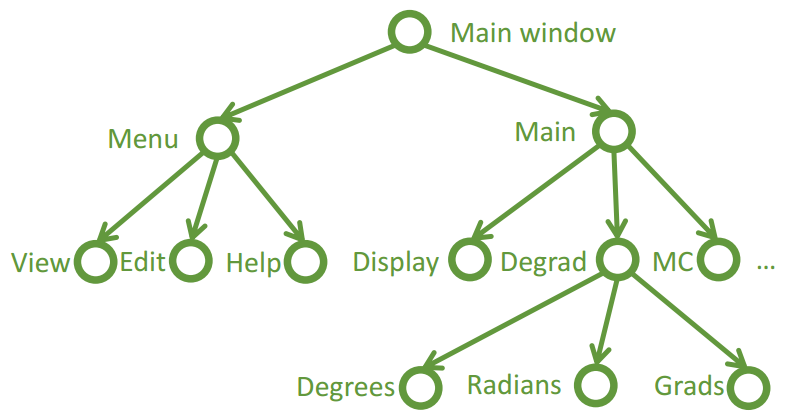
\includegraphics[scale=0.25]{GUI-hierarchia}
		\caption{A komponensek hierarchiája}
		\label{fig:GUI-hierarchia}
	\end{subfigure}
	\caption{A metróhálózatot ábrázoló gráf kiterjesztései}
\end{figure}

\begin{feladat}
	Mi történik, amikor egy alkalmazás ablakán kattintunk -- hogyan határozza meg a rendszer, hogy melyik komponensre kattintottunk?
\end{feladat}




%%%%%%%%%%%%%%%%%%%%%%%%%%%%%%%%%%%%%%%%%%%%%%%%%%%%%%%%%%%%%%%%%%%%%%%%%%%%%%%%%%%%%%%%%%%%%%%%%%%%




\section{Összefoglalás}

A fejezetben bemutattuk \fogalom{struktura-alapu-modellezes} motivációját, a használt formalizmusukat és azok alkalmazásait. Ismertettük \fogalomragozva{tipus}{típusok} fontosságát és a típusrendszer ábrázolásának lehetőségeit.

A következő fejezetekben a \fogalomragozva{viselkedes-alapu-modellezes}{viselkedés alapú modellezést} és annak formalizmusait mutatjuk be.

%%%%%%%%%%%%%%%%%%%%%%%%%%%%%%%%%%%%%%%%%%%%%%%%%%%%%%%%%%%%%%%%%%%%%%%%%%%%%%%%%%%%%%%%%%%%%%%%%%%%

\section{Kitekintés: technológiák és technikák\kieg}

Az alábbiakban bemutatunk néhány, a strukturális modellezés témaköréhez kapcsolódó gyakorlati technológiát, specifikációt és eszközt. Az itt felsorolt fogalmak nem részei a számonkérésnek, gyakran előkerülnek viszont a későbbi tanulmányok és munkák során, ezért mindenképpen érdemes legalább névről ismerni őket.

\subsection{Technológiák}

A gyakorlatban sokféle modellezési nyelvet és technológiát használnak. Ezek közül mutatunk be most azokat, amelyek a később tanulmányok során előkerülnek.

\subsubsection{UML}

Az \roviditesangolulkifejtve{UML} egy általános célú modellezési nyelv az~\cite{UML}. Az UML három fő diagramtípust definiál:

\begin{itemize}
	\item \emph{Structure Diagram:} strukturális modellek leírására. A \emph{Class Diagram} az osztályok (metamodell), míg az \emph{Object diagram} a példányok (modell) leírására alkalmas. A \emph{Composite Structure Diagram} egy rendszer struktúráját és a rendszer komponenseinek kapcsolatát mutatja be.
	\item \emph{Behaviour Diagram:} viselkedési modellek leírására, pl. a \emph{State Machine Diagram} segítségével állapotgépek az \emph{Activity Diagramon} folyamatok ábrázolhatók. A \emph{Behaviour Diagramek} között megkülönböztejük az \emph{Interaction Diagrameket}. Ezeknek szintén a viselkedés leírása a célja, de a hangsúly a vezérlés- és adatáramlás bemutatásán van. Ilyen pl. a \emph{Sequence Diagram} (szekvenciadiagram), amely az egyes objektumok közötti interakciót mutatja be üzenetek formájában.
\end{itemize}

\remofigscale{UML-diagram}{UML diagramok típusai és a közöttük lévő viszony osztálydiagramként ábrázolva~\cite{wiki:ISE}}{0.6}

Az UML nyelvvel részletesen foglalkozik a \szofttech tárgy.

%\subsubsection{AADL}
%Az \roviditesangolulkifejtve{AADL} eredetileg repülőipari célokra fejlesztett architektúraleíró nyelv~\cite{AADL}.

\subsubsection{EMF}

Az Eclipse fejlesztőkörnyezet~\cite{eclipse} saját modellezési keretrendszerrel rendelkezik, ez az \roviditesangolulkifejtve{EMF}. Az EMF metamodellező nyelve, az Ecore lehetővé teszi saját, ún. \roviditesteljesenkifejtve{DSL} definiálását. Az EMF mára több területen is \emph{de facto} modellezési keretrendszer.

Az Eclipse fejlesztőkörnyezettel és az EMF keretrendszerrel foglalkozik az \eat szabadon választható tárgy.

\subsection{Struktúramodellezési technikák}

A struktúramodellek definiálására és fejlesztésére különböző technikák léteznek. Korábban tárgyaltuk a \fogalomangolul{top-down} és a \fogalomangolul{bottom-up} tervezést. Itt két további, általánosan alkalmazható technikát mutatunk be.

\subsubsection{Tervezési minták}

Az \fogalom{objektum-orientalt} tervezés során gyakran előforduló problémákra különböző \fogalomragozva{tervezesi-minta}{tervezési minták} (\fogalomragozva{tervezesi-minta}{design patterns}) léteznek. A tervezési minták között külön szerepet kapnak a rendszer struktúráját leíró \fogalomragozva{szerkezeti-minta}{szerkezeti minták} (\fogalomragozva{szerkezeti-minta}{structural patterns}). A tervezési mintákkal bővebben a \sznikak tárgy foglalkozik.

\subsubsection{Refaktoring}

A \fogalomragozva{dekompozicio}{dekompozícióhoz}, azaz \fogalomragozva{faktoring}{faktoringhoz} szorosan kapcsolódik a \fogalom{refaktoring} (\fogalomangolul{refaktoring}) fogalma~\cite{fowler2012refactoring}. Refaktoring során egy rendszert definiáló programkód vagy modell átalakítását értjük. A refaktoring lényege, hogy az átalakítás során a rendszer megfigyelhető működése változatlan marad, de a kapott programkód vagy modell érthetőbb, karbantarthatóbb lesz.

%\section{További technológiák}
%
%\subsubsection{SysML}
%
%A \roviditesangolulkifejtve{SysML} egy UML-alapú általános modellezési nyelv rendszertervezési célokra~\cite{SysML}. A SysML az UML egy részhalmazát bővíti ki és új diagramtípusokat is bevezet, pl. \emph{Requirement Diagram} követelmények és viszonyaik ábrázolására alkalmas.
%
%%\subsubsection{RDF}
%%
%%\roviditesangolulkifejtve{RDF}
%%
%%TODO erről is lesz szakirányos tárgy
%
%\subsubsection{AUTOSAR}
%
%Az \roviditesangolulkifejtve{AUTOSAR}~\cite{autosar} nagy autóipari gyártók és beszállítóik által fejlesztett szabványos architektúranyelv, amely az egyes hardver- és szoftverkomponensek együttműködése magas szinten definiálható. Az AUTOSAR konzorciumnak a \emph{Méréstechnika és Információs Rendszerek Tanszék} is tagja~\cite{autosar-attendees}.


\subsection{Struktúramodellező eszközök és vizualizáció}

Gráfok automatikus megjelenítésére alkalmas pl. a GraphViz\footnote{\url{http://www.graphviz.org/}} programcsomag. Gráfok feldolgozására gyakran alkalmazzák az igraph\footnote{\url{http://igraph.org/}} programcsomagot. Manapság több gráfadatbázis-kezelő rendszer is elterjedt, pl. a Neo4j\footnote{\url{http://neo4j.com/}} és a Titan\footnote{\url{http://thinkaurelius.github.io/titan/}} rendszerek.

Gráfok manuális rajzolására szintén több eszköz elterjedt. Egyszerűen használható online felületet biztosít a draw.io\footnote{\url{http://draw.io/}} és az Arrow Tools\footnote{\url{http://www.apcjones.com/arrows/}}. A jegyzetben szereplő ábrák a yEd eszközzel\footnote{\url{https://www.yworks.com/products/yed}} készültek. Sok információt tartalmazó gráf esetén érdemes lehet vektorgrafikus rajzoló-, ill. prezentáló eszközök, pl. a Microsoft Visio vagy Microsoft PowerPoint alkalmazás.

%%%%%%%%%%%%%%%%%%%%%%%%%%%%%%%%%%%%%%%%%%%%%%%%%%%%%%%%%%%%%%%%%%%%%%%%%%%%%%%%%%%%%%%%%%%%%%%%%%%%

\section{Elméleti kitekintés\kieg}

A struktúramodellezésnek komoly matematikai eszköztára is van. Az alábbiakban ezekből mutatunk be néhány részletet.

%\subsection{Hipergráfok}
%
%A gráf adatmodell kiterjesztése a \fogalom{hipergraf}. A hipergráfban a \fogalomragozva{hiperel}{hiperélek} több csomópont között is futhatnak. Megkülönböztetünk irányított és irányítatlan hipergráfokat.
%
%Az irányítatlan hipergráfok egyszerűen leképezhetők \fogalomragozva{paros-graf}{páros gráffá}: a gráf egyik halmazában a hipergráf csomópontjainak, a másik halmazában a hiperéleknek veszünk fel egy pontot.
%

%\fogalom{kenyszer} + \rovidites{CSP}
%\todo[inline]{ábra}

%\subsection{Relációk}

\subsection{Bináris relációk tulajdonságai}

%A \fogalom{tranzitiv-lezaras} fogalom jelentésének megértését segíti, ha \\
Hasznos ismerni a kétváltozós relációkon értelmezett tulajdonságokat~\cite{wiki:relacio}.

\begin{tipp}
	Az elnevezések egyezése nem véletlen, a \fogalom{ketvaltozos-relacio} egy alesete a \fogalom{relacio} fogalomnak.
\end{tipp}

%http://math.stackexchange.com/questions/65102/if-a-relation-is-symmetric-and-transitive-will-it-be-reflexive

\begin{definicio}
	Egy $S$ halmazon értelmezett $r$ kétváltozós reláció \fogalomragozva{reflexivitas}{reflexív}, ha bármely $a \in S$-re $r(a, a)$ teljesül.
\end{definicio}

\begin{definicio}
	Egy $S$ halmazon értelmezett $r$ kétváltozós reláció \fogalomragozva{szimmetria}{szimmetrikus}, ha bármely $a,b \in S$-re $r(a, b)$ teljesülése esetén $r(b, a)$ is teljesül. A nem szimmetrikus relációkat \fogalomragozva{aszimmetria}{aszimmetrikusnak} nevezzük.
\end{definicio}

\begin{definicio}
	Egy $S$ halmazon értelmezett $r$ kétváltozós reláció \fogalomragozva{tranzitivitas}{tranzititív}, ha bármely $a,b,c \in S$-re $r(a, b)$ és $r(b, c)$ teljesülése esetén $r(a, c)$ is teljesül.
\end{definicio}

\begin{pelda}
	\remofigscalefixed{tranzitivitas}{Az \emph{egyenlő} ($=$) és a \emph{kisebb} ($<$) relációk gráfon ábrázolva}{\yedscale}

	Tranzitív relációk:
	\begin{itemize}
	\item Az \emph{egyenlő} ($=$) és a \emph{kisebb} ($<$) relációk tranzitívak, mert
	\begin{itemize}
		\item $a = b$ és $b = c$ esetén $a = c$,
		\item $d < e$ és $e < f$ esetén $e < f$.
	\end{itemize}
	\Az+\ref{fig:tranzitivitas}. ábrán ábrázoltuk a fenti relációkat. Az $=$ reláció szimmetrikus, ezért irányítatlan gráffal, a $<$ reláció aszimmetrikus, ezért irányított gráffal reprezentálható.
	\end{itemize}
	
	Nem tranzitív relációk:
	\begin{itemize}
	\item A \emph{nemegyenlő} reláció ($\neq$) nem tranzitív, mert 
	\begin{itemize}
		\item $a \neq b$ és $b \neq c$ esetén $a \neq c$ nem mindig áll fenn, például
		\item $1 \neq 2$ és $2 \neq 1$ esetén $1 \neq 1$ nem teljesül.
	\end{itemize}
	\item Személyek közötti $\mathit{őse}$ reláció tranzitív, mert $\mathit{őse}(a, b)$ és $\mathit{őse}(b, c)$ esetén $\mathit{őse}(a, c)$ is fennáll. 
	\item Személyek közötti $\mathit{ismerőse}$ reláció nem tranzitív, mert $\mathit{ismerőse}(a, b)$ és $\mathit{ismerőse}(b, c)$ esetén nem garantált, hogy $\mathit{ismerőse}(a, c)$ fennáll.
	\end{itemize}
\end{pelda} 

%%%%%%%%%%%%%%%%%%%%%%%%%%%%%%%%%%%%%%%%%%%%%%%%%%%%%%%%%%%%%%%%%%%%%%%%%%%%%%%%%%%%%%%%%%%%%%%%%%%%

\section{Ajánlott irodalom}

A gráfelmélettel behatóan foglalkozik a \bszketto tantárgy és Fleiner Tamás jegyzete~\cite{FleinerJegyzet}. Különböző gráfalgoritmusokat mutat be -- pl. \fogalom{legrovidebb-ut} és minimális összsúlyú \fogalom{feszitofa} keresésére -- az \algel tárgy. További keresőalgoritmusok a \mestersegesintelligencia tárgyban szerepelnek.

Olvasmányos összefoglalót nyújt az UML nyelvről Martin Fowler ,,UML distilled'' című könyve~\cite{fowler1997uml}.

A tulajdonsággráfokról egy jól érthető tudományos cikk Marko Rodriguez és Peter Neubauer munkája~\cite{Rodriguez2010}. Rodriguez a Titan elosztott gráfadatbázis-kezelő rendszer egyik fő fejlesztője~\cite{Titan}, míg Neubauer a Neo4j gráfadatbázis-kezelőt fejlesztő cég alapítója~\cite{Neo4j}. Az elosztott gráfadatbázis alkalmazását, elméleti és gyakorlati kihívásait kiváló prezentációkban mutatja be~\cite{RodriguezSlides2012,RodriguezSlides2013}.

Barabási-Albert László magyar fizikus nemzetközileg elismert kutatója a komplex \fogalomragozva{halozat}{hálózatok} elméletének. Barabási ,,Behálózva'' című könyve közérthető stílusban mutatja be a hálózatok elemzésének elméleti kihívásait a kutatási eredmények gyakorlati jelentőségét~\cite{behalozva}. A szerzővel több interjú is készült~\cite{barabasi1,barabasi2,barabasi3}.

%Az osztályok és prototípusok közötti elvi különbséget mutatja be Antero Taivalsaari, a Nokia Research fejlesztőjének 1996-os cikke~\cite{taivalsaari1996classes}.

%\roviditesangolulkifejtve{SQL}
%\fogalom{azonosito} (\fogalomragozva{elsodleges-kulcs}{elsődleges kulcsok})

\topic{Állapotalapú modellezés}\label{sec:allapot-alapu-modellezes}

\graphicspath{ {./allapot-alapu-modellezes/figures/} }

\newcommand{\allapotgepsmallscale}{0.45}
\newcommand{\allapotgepmediumscale}{0.53}
\newcommand{\allapotgeplargescale}{0.6}

\newenvironment{fektetett}{\begin{landscape}\vspace*{\fill}}{\vspace*{\fill}\end{landscape}}

Az alábbi dokumentum egy háromfényű közúti jelzőlámpa fokozatosan kidolgozott modelljén keresztül mutatja be az állapot alapú modellezés alapfogalmait.

A bemutatott modellek a Yakindu Statechart Tools\footnote{\url{http://statecharts.org}} eszközzel készültek.

\section{Egyszerű állapotgépek}

A példa kidolgozását azzal az egyszerű esettel kezdjük, amikor a modellező nyelv lényegében a \emph{Digitális technika} tárgyből megismert \fogalom{mealy-automata} formalizmus.

\subsection{Állapottér}

Ehhez első lépéseként meg kell határozni a rendszer \fogalomragozva{allapotter}{állapotterét}. Az állapottér elemeit \fogalomragozva{allapot}{állapotoknak} nevezzük. Az állapottérnek az alábbi két kritériumnak kell megfelelnie: 

\begin{definicio}
\Fogalom{teljesseg}. Minden időpontban az állapottér legalább egy eleme jellemzi a rendszert.
\end{definicio}

\begin{definicio}
\Fogalom{kizarolagossag}. Minden időpontban az állapottér legfeljebb egy eleme jellemzi a rendszert.
\end{definicio}

Egy adott időpontban a rendszer \fogalomragozva{pillanatnyi-allapot}{pillanatnyi állapota} az állapottér azon egyetlen eleme, amelyik abban az időpontban jellemző a rendszerre. A rendszer egy \fogalomragozva{kezdoallapot}{kezdőállapota} olyan állapot, amely a vizsgálatunk kezdetekor (például a $t = 0$ időpillanatban) pillanatnyi állapot lehet.

\begin{pelda}
Határozzuk meg egy jelzőlámpa egyszerű állapotterét!
\end{pelda}


\newcommand{\allapotikon}[1]{\includegraphics[height=0.3cm]{#1}}

\begin{itemize}
\item \allapotikon{tl_empty} \allapot{Off}: kikapcsolt állapot
\item \allapotikon{tl_red} \allapot{Stop}: piros jelzés
\item \allapotikon{tl_redyellow} \allapot{Prepare}: piros-sárga jelzés
\item \allapotikon{tl_green} \allapot{Go}: zöld jelzés
\item \allapotikon{tl_yellow} \allapot{Continue}: sárga jelzés
\end{itemize}

Kezdetben a rendszer legyen kikapcsolva, vagyis a rendszer egyetlen kezdőállapota legyen \allapot{Off}.

\subsection{Állapotámenet, esemény}

A rendszer időbeli viselkedésében kulcsfontosságú, hogy a pillanatnyi állapot hogyan változik az idővel. Bizonyos mérnöki diszciplínákban ez a változás folytonos függvénnyel jellemezhető (ilyen rendszerekkel a \emph{Rendszerelmélet} című tárgy foglalkozik részletesebben). Például egy repülő állapota lehet a tengerszint feletti magasság, amely egy időben folytonosan változó mennyiség. Azonban az informatikai gyakorlatban a \fogalomragozva{diszkret-allapotter}{diszkrét állapottereknek} van kiemelt jelentősége, ahol nem létezik folytonos átmenet az állapotok között, tehát a rendszer pillanatnyi állapota mindaddig állandó, amíg egy pillanatszerű esemény hatására egy másik állapotba át nem megy.

Az ilyen diszkrét rendszerek viselkedése \fogalomragozva{allapotatmenet}{állapotátmenetekkel} (más néven \fogalomragozva{tranzicio}{tranzíciókkal}) jól modellezhető. Egy állapotátmenet megengedi, hogy a rendszer állapotot váltson egy forrás- és egy célállapot között. Amennyiben a rendszer pillanatnyi állapota a forrásállapot, az állapotátmenet \fogalomragozva{tuzeles}{tüzelését} követően a rendszer új állapota a célállapot lesz. (Az, hogy a tüzelés pillanatában a rendszer pillanatnyi állapota a forrás- vagy a célállapot-e, megállapodás kérdése.)

Egy állapotátmenet tüzelését egy adott \fogalom{esemeny} bekövetkezte váltja ki. (Ennek speciális esete a spontán állapotátmenet, amikor a kiváltó esemény kívülről nem megfigyelhető.) Ezen felül állapotátmenetek \fogalomragozva{akcio}{akciókat} hajthatnak végre, például maguk is válhatnak ki eseményeket. Sokszor praktikus egy adott rendszer szempontjából bemenet és kimeneti események elkülönítése.

\begin{pelda}
Definiáljuk a jelzőlámpa modelljéhez az alábbi bemeneti eseményeket:

\begin{itemize}
	\item \allapot{onOff}: ki- és bekapcsolás kérése
	\item \allapot{switchPhase}: jelzésváltás kérése
\end{itemize}

A jelzőlámpa a működését a balesetek reprodukálását segítendő folyamatosan naplózza egy külső fekete dobozba. Ennek megfelelően legyenek a rendszer output eseményei a következők:

\begin{itemize}
	\item \allapot{Stop}: a rendszer sárga jelzésből vörös jelzésbe váltott
	\item \allapot{Go}: a rendszer zöld jelzésbe váltott
\end{itemize}

Az események definíciója a Yakindu szerkesztőjében a következőképpen adható meg:

\begin{lstlisting}
interface:
  in event onOff
  in event switchPhase
  out event stop
  out event go
\end{lstlisting}

Ekkor a jelzőlámpa modellezhető \az+\refstruc{fig:TrafficLight_1} állapotgépével.
\end{pelda}

\remofigscale{TrafficLight_1}{Jelzőlámpa egyszerű állapotgépe}{\allapotgeplargescale}

A diagramon a rendszer állapotait (\allapot{Off}, \allapot{Stop}, \allapot{Prepare}, \allapot{Go}, \allapot{Continue}) lekerekített téglalapok jelölik. Az állapotgép kezdőállapotát (\allapot{Off}) a tömör fekete korongból húzott nyíl jelöli ki. A téglalapok között húzott nyilak a megfelelő állapotok közötti tranzíciókat jelképezik. A nyilakra írt címkék a tranzíciót kiváltó, illetve a kiváltott eseményekre hivatkoznak (Yakinduban az esemény kiváltását \lstinline{raise} kulcsszó jelöli).

Amint azt a fenti definíciókból láthatjuk, az ,,állapot'' kifejezés két különböző jelentéssel bír:

\begin{itemize}
	\item \Fogalom{szintaktikai-jelentes}. Az állapotgráf egy csomópontja, melyet lekerekített téglalap jelöl (\fogalom{allapotcsomopont}).
	\item \Fogalom{szemantikai-jelentes}. Az állapottér egy eleme.
\end{itemize}

Egyszerű állapotgépek esetében elmondható, hogy a két fogalom által jelölt objektumok megfeleltethetőek egymásnak. Az állapotgép formalizmus új szintaktikai elemekkel történő kiterjesztésével (változók, összetett állapotok, ortogonális állapotok -- ld. később) ugyanakkor ez a kapcsolat a továbbiakban nem áll fenn.

\remofigscale{TrafficLight_1_sim}{Pillanatnyi állapot nyomonkövetése szimulációval}{\allapotgeplargescale}

\begin{tipp}
A Yakindu eszköz lehetőséget biztosít az állapotgép \fogalomragozva{szimulacio}{szimulációjára}. Szimuláció során nyomon tudjuk követni, hogy a adott események hatására időben hogyan alakul a rendszer pillanatnyi állapota.

Például az \allapot{onOff}, majd \allapot{switchPhase} események a szimulátor felületén történő kiváltását követően a rendszer \allapot{Prepare} állapotba kerül, amit a Yakindu az állapotot jelképező téglalap átszínezésével ábrázol (ld. \refstruc{fig:TrafficLight_1_sim}).
\end{tipp}

A fenti modell két fontos tulajdonsággal bír:

\begin{definicio}
	\Fogalom{determinisztikus}. Az állapotgépnek legfeljebb egy kezdőállapota van, valamint bármely állapotban, bármely bemeneti esemény bekövetkeztekor legfeljebb egy tranzíció tüzelhet.
\end{definicio}

\begin{megjegyzes}
	A Yakindu csak determinisztikus modellek létrehozását támogatja.
\end{megjegyzes}

\begin{definicio}
	\Fogalom{teljesen-specifikalt}. Az állapotgépnek legalább egy kezdőállapota van, valamint bármely állapotban, bármely bemeneti esemény bekövetkeztekor legalább egy tranzíció tüzelhet.
\end{definicio}

\begin{megjegyzes}
	Ennek egyik következménye, hogy a rendszer \fogalom{holtpontmentes}, azaz nem tartalmaz olyan állapotot, amelyből nem vezet ki tranzíció.
\end{megjegyzes}

\subsection{Végrehajtási szekvencia}

A rendszer időbeli viselkedését annak \fogalomragozva{vegrehajtasi-szekvencia}{végrehajtási szekvenciái} jellemzik. Egy végrehajtási szekvencia állapotok és események egy

$$s_0 \xrightarrow{i_0 / o_0} s_1 \xrightarrow{i_1 / o_1} \ldots$$

(véges vagy végtelen) alternáló sorozata, ahol $s_0$ a rendszer egy kezdőállapota, $s_j \xrightarrow{i_j / o_j} s_{j+1}$ pedig a rendszer egy állapotátmenete minden $j$-re. Egy állapot \fogalom{elerheto}, ha a rendszernek létezik véges végrehajtási szekvenciája az állapotba.

\begin{pelda}
	Az $\mathit{Off} \xrightarrow{\mathit{onOff}} \mathit{Stop} \xrightarrow{\mathit{switchPhase}} \mathit{Prepare} \xrightarrow{\mathit{switchPhase} / \mathit{go}} \mathit{Go}$ sorozat a jelző egy véges végrehajtási szekvenciája; ennek megfelelően biztosan tudjuk, hogy például a \allapot{Go} állapot elérhető állapot. Az $\mathit{Off} \xrightarrow{\mathit{onOff}} \mathit{Stop} \xrightarrow{\mathit{onOff}} \mathit{Off} \xrightarrow{\mathit{onOff}} \ldots$ egy végtelen végrehajtási szekvencia.
\end{pelda}

Az állapotgép végrehajtási szekvenciái vezérelten bejárhatóak szimuláció segítségével, ami jó módot ad az állapotgép ellenőrzésére. A Yakindu beépített szimulátora erre lehetőséget biztosít.

\section{Hierarchia}

\remofigscale{TrafficLight_15}{Jelzőlámpa állapotgépe \esemeny{reset} eseménnyel \halalfejes}{\allapotgeplargescale}

\begin{pelda}
	Egészítsük ki a fenti modellt egy \allapot{reset} bemeneti eseménnyel, melynek hatására bekapcsolt állapotban a jelzőlámpa alaphelyzetbe (\allapot{Stop} állapotba) áll.

	Az eddig megismert eszközökkel elkészített modellt szemlélteti \az+\refstruc{fig:TrafficLight_15}.
\end{pelda}

Vegyük észre, hogy a rendszer a \allapot{reset} eseményre a \allapot{Stop}, \allapot{Prepare}, \allapot{Go} és \allapot{Continue} állapotok mindegyikében egyformán viselkedik. Ebben az esetben ez annak köszönhető, hogy ezen állapotok mindegyikében a rendszer bekapcsolt állapotban van. Ezt a kapcsolatot a modellben explicit módon meg lehet jeleníteni egy \fogalom{osszetett-allapot} bevezetésével, amely a négy állapot közös tulajdonságait és viselkedését általánosítja.

\subsection{Összetett állapot, állapotrégió}

Egy összetett állapot szintaktikailag megfelel egy egyszerű állapotnak, azzal a kivétellel, hogy saját \fogalomragozva{regio}{régióval} rendelkezik, mely további állapotokat (beleértve a kezdőállapotokat) és köztük tranzíciókat tartalmazhat. Régiók közül kiemelt jelentőséggel bír a legfelső szintű régió, mely magát az állapotgépet tartalmazza.

\Az+\refstruc{fig:TrafficLight_2_sim} szemlélteti az \allapot{On} összetett állapot bevezetésével kapott modellt.

\remofigscale{TrafficLight_2_sim}{Hierarchikus állapot pillanatnyi állapotként}{\allapotgeplargescale}

A teljes állapotgépet az \allapot{Operation}, míg az összetett állapot belsejét a \allapot{Phase} régió tartalmazza. A \allapot{Phase} régió kezdőállapota a \allapot{Stop} állapot, így a régióba való belépéskor ez az állapot lesz a rendszer pillanatnyi állapota. A \allapot{reset} esemény az \allapot{On} állapotból \allapot{On} állapotba vezet, így hatására valóban a \allapot{Stop} állapot lesz aktív.

A fenti példát szimulálva az \allapot{onOff} esemény \allapot{Off} állapotban történő fogadását követően az elvárásoknak megfelelően a \allapot{Stop} állapot a rendszer pillanatnyi állapota lesz. Ugyanakkor a \allapot{Stop} állapotot tartalmazó \allapot{On} állapot is pillanatnyi állapot lesz:

\remofigscale{TrafficLight_2}{Jelzőlámpa állapotgépe összetett állapottal}{\allapotgeplargescale}

Általánosságban ha egy tartalmazott (egyszerű vagy összetett) állapot aktív, akkor az őt tartalmazó összetett állapot is aktív. Ezt fejezi ki az \fogalom{allapotkonfiguracio} fogalma, ami állapotok egy olyan maximális (azaz nem bővíthető) halmaza, melyek egyszerre lehetnek aktívak a rendszerben.

\begin{pelda}
A jelzőlámpa állapotkonfigurációi:

\begin{itemize}
\item \{ \allapot{Off} \}
\item \{ \allapot{On}, \allapot{Stop} \}
\item \{ \allapot{On}, \allapot{Prepare} \}
\item \{ \allapot{On}, \allapot{Go} \}
\item \{ \allapot{On}, \allapot{Continue} \}
\end{itemize}
\end{pelda}

Tartalmazó és tartalmazott állapot között tehát nem érvényesül a kizárólagosság. Ennek megfelelően a hierarchikus állapot bevezetésével többféle érvényes állapottér adódik.

\begin{pelda}
A jelzőlámpa érvényes állapotterei:

\begin{itemize}
	\item  \{ \allapot{Off}, \allapot{On} \}
	\item  \{ \allapot{Off}, \allapot{Stop}, \allapot{Prepare}, \allapot{Go}, \allapot{Continue} \}
\end{itemize}

Ezen felül az állapotkonfigurációk halmaza is tekinthető állapottérnek:

\begin{itemize}
	\item \{ \{ \allapot{Off} \}, \{ \allapot{On}, \allapot{Stop} \}, \{ \allapot{On}, \allapot{Prepare} \}, \{ \allapot{On}, \allapot{Go} \}, \{ \allapot{On}, \allapot{Continue} \} \}
\end{itemize}

Ugyanakkor az \{ \allapot{Off}, \allapot{On}, \allapot{Stop}, \allapot{Prepare}, \allapot{Go}, \allapot{Continue} \} nem jó állapottér, hiszen ebben az esetben például az \{ \allapot{On}, \allapot{Prepare} \} részhalmaz sérti a kizárólagosságot. Általános szabály, hogy egy állapottér vagy az összetett állapotot, vagy annak összes részállapotát tartalmazza, de nem mindkét változatot.
\end{pelda}

A \{ \allapot{Stop}, \allapot{Prepare}, \allapot{Go}, \allapot{Continue} \} részállapottér az \allapot{On} állapotot \fogalomragozva{finomitas}{finomítja}, míg az \allapot{On} állapot a \{ \allapot{Stop}, \allapot{Prepare}, \allapot{Go}, \allapot{Continue} \} állapotokat \fogalomragozva{absztrakcio}{absztrahálja}. Jó modellezési gyakorlat a modell állapotainak fokozatos finomítása.

\subsection{Többszintű állapothierarchia}

Amint a következő példából kiderül, az állapotok közötti hierarchia nem feltétlenül egyszintű.

\begin{pelda}
\Az+\ref{fig:TrafficLight_3}. ábrán szemléltetett modell az \allapot{On} állapotot tovább bővíti egy \allapot{Alert} állapottal, mely a jelző sárgán villogó, figylemeztető állapotát modellezi. A rendes üzem jelzéseit a \allapot{Normal} összetett állapot tartalmazza. A \allapot{Normal} és \allapot{Alert} állapotok közötti váltás a \esemeny{switchMode} bemeneti esemény hatására történik, a $\mathit{Normal} \rightarrow \mathit{Alert}$ állapotváltás \allapot{Alert} kimeneti eseményt vált ki.
\end{pelda}

\remofigscale{TrafficLight_3}{Jelzőlámpa állapotgépe többszintű összetett állapottal}{\allapotgeplargescale}

\section{Változók és őrfeltételek}

Finomítsuk az \allapot{Alert} állapotot \allapot{LightOn} és \allapot{LightOff} alállapotokkal, melyek fél másodpercenként váltakozva a sárga fény villogását modellezik!
A villogás modellezéséhez feltételezzünk egy \allapot{tick} bejövő eseményt, amely a specifikáció szerint egy 8 Hz frekvenciájú órajel, tehát egyenletes ütemben, másodpercenként nyolcszor jelez.

Ahhoz, hogy a 2 Hz-es váltakozást modellezzük, a \allapot{tick} esemény minden negyedik bekövetkeztekor kell váltani \allapot{LightOn} és \allapot{LightOff} között. Ezért az állapotokat tovább kell finomítanunk, hogy a bekövetkező órajeleket számolni tudjuk.

\remofigscale{TrafficLight_35}{Villogó jelzés külső órával \halalfejes}{\allapotgepmediumscale}

Egy lehetséges megvalósítást szemléltet \az+\refstruc{fig:TrafficLight_35}.

A fenti állapotgép valóban a kívánt viselkedést modellezi: az állapotgép \allapot{Alert} állapotban pontosan minden negyedik \allapot{tick} eseményre vált \allapot{LightOn} és \allapot{LightOff} állapotok között.

Abban az esetben azonban, ha csak minden századik eseményre kellene váltani \allapot{LightOn} és \allapot{LightOff} között, mindkét összetett állapot száz alállapotot tartalmazna. Látható tehát, hogy ez nem lesz jó modellezési gyakorlat, hiszen az így bemutatott modell elkészítése nagy erőfeszítést igényel, sok hibalehetőséget rejt és nehezen átlátható; valamint a számszerű paraméterek megváltozása esetén jelentős módosítást igényel.

\subsection{Belső változók}

A probléma megoldható \fogalomragozva{valtozo}{változók} alkalmazásával. A változó típussal rendelkezik, ez Yakinduban lehet \tipus{boolean}, \tipus{integer}, \tipus{real} vagy \tipus{string}, ezek a programozási nyelveknél megszokott logikai, egész, lebegőpontos, illetve karakterlánc típusoknak felelnek meg. Változók jelenlétében a rendszer állapotát már nemcsak a vezérlés állapota (állapot csomópontok), hanem az éppen érvényes \fogalom{valtozoertekeles} is meghatározza.

\begin{pelda}
A bekövetkezett \allapot{tick} események számlálására a rendszer interfészdefinícióját kiegészítjük a \allapot{counter} egész típusú változóval:

\begin{minipage}{\linewidth}
\begin{lstlisting}
var counter : integer
\end{lstlisting}
\end{minipage}
\end{pelda}

A változó értékét \fogalomragozva{utasitas}{utasítással} lehet módosítani, amely -- az eseménykiváltáshoz hasonlóan -- tranzícióhoz kapcsolható \fogalom{akcio}. Akció ezen felül kapcsolható állapothoz is az \valtozo{entry} és \valtozo{exit} triggerek segítségével, melyek az állapotba való belépéskor, illetve az állapotból történő kilépéskor aktiválódnak. %TODO define trigger

Azt, hogy a változó aktuális értéke befolyással lehessen a vezérlésre, a tranzíciókra felírt őrfeltételekkel lehet megvalósítani. Az őrfeltétel biztosítja, hogy a tranzíció csak akkor tüzelhessen, ha az őrfeltételbe felírt logikai kifejezést az aktuális állapot változóértékelése kielégíti.

\begin{pelda}
A \allapot{tick} események számlálása változóval megvalósítható \az+\refstruc{fig:TrafficLight_4} állapotgépe szerint. Figyeljük meg, hogy a változó értékét szögletes zárójelekbe tett őrfeltételek használják.
\end{pelda}

\remofigscale{TrafficLight_4}{Villogó jelzés számlálóval}{\allapotgepmediumscale}

\begin{pelda}
A fenti rendszer egy végrehajtásiszekvencia-részlete:
\begin{align*}
& \langle \mathit{LightOn}, \{ \mathit{counter} \mapsto 0 \} \rangle \xrightarrow{\mathit{tick}}
  \langle \mathit{LightOn}, \{ \mathit{counter} \mapsto 1 \} \rangle \xrightarrow{\mathit{tick}}
  \langle \mathit{LightOn}, \{ \mathit{counter} \mapsto 2 \} \rangle \xrightarrow{\mathit{tick}} \\
& \langle \mathit{LightOn}, \{ \mathit{counter} \mapsto 3 \} \rangle \xrightarrow{\mathit{tick}}
  \langle \mathit{LightOff}, \{ \mathit{counter} \mapsto 0 \} \rangle
\end{align*}

\end{pelda}

\begin{feladat}
Hogyan módosul őrfeltételek jelenlétében a \fogalomragozva{determinisztikus}{determinizmus} definíciója?
\end{feladat}

\subsection{Interfészváltozók}

A vörös, sárga ill. zöld színű fények állapotának nyilvántartására felvesszük \valtozo{red}, \valtozo{yellow} és \valtozo{green} logikai változókat. A korábban bevezetett \valtozo{counter} változóval ellentétben ezek a változók nem csak az állapotgéppel leírt vezérlő belső működésében játszanak szerepet; úgy tekintjük, hogy a különböző színű fények villanyégőit közvetlenül ezek az \fogalomragozva{interfeszvaltozo}{interfészváltozók} kapcsolják. Általánosságban a be- és kimeneti események mellett interfészváltozókon keresztül kommunikálhat az állapotgép a külvilággal.

Mivel a vezérlési állapotokat úgy vettük fel, hogy egyértelműen meghatározzák a fényeket leíró változók értékét, ezen változóknak értéket adó utasításokat \valtozo{entry} triggerhez rendeljük -- ez egy tömör jelölése annak, hogy az adott állapotba lépő összes állapotátmenet végrehajtson egy adott akciót.

\remofigscale{TrafficLight_5}{Fények állapotának modellezése változókkal}{\allapotgepmediumscale}

A bővített állapotgépet \az+\refstruc{fig:TrafficLight_5} szemlélteti.

\section{Időzítés}

A modell időbeli viselkedését eddig egy külső óra által szolgáltatott, megszabott frekvenciájú órajelet feltételezve modelleztük. A Yakindu azonban lehetőséget biztosít időzített események explicit modellezésére az \valtozo{after} kulcsszóval. Ezen felül az \valtozo{after} és \valtozo{every} trigger használatával időzített esemény állapothoz is rendelhető.

Az időzítés explicit modellezésével a modell tömörebb, kifejezőbb lehet, és a későbbi tényleges technikai megvalósítás apró részleteitől (órajel frekvenciája) függetlenül érvényes.

Az időzítést használó modellt \az+\refstruc{fig:TrafficLight_6} szemlélteti.

\remofigscale{TrafficLight_6}{Villogó jelzés időzítéssel}{\allapotgepmediumscale}

\section{Ortogonális dekompozíció}

Bővítsük a modellt járműérzékelő\footnote{\url{https://en.wikipedia.org/wiki/Induction\_loop\#Vehicle\_detection}} funkcióval!

\begin{tipp}
	A jelzőlámpa (bekapcsolt állapotban) periodikus \esemeny{trafficPresent} és \esemeny{trafficAbsent} bemeneti események fogadásával értesül arról, hogy tartózkodik-e jármű a lámpa előtti útszakaszon. A jelző ezt az információt a \valtozo{queue} logikai változóban tárolja (ennek értéke kezdetben $\mathsf{true}$). A foglaltság nyilvántartásának értelme, hogy ilyenkor csak akkor kell \allapot{Stop} állapotból \allapot{switchPhase} esemény hatására jelzést váltani, ha van a lámpa előtt várakozó jármű, vagyis $\mathit{queue} = \mathsf{true}$.
\end{tipp}

A járműérzékelő jeleinek fogadását \az+\ref{fig:TrafficLight_7_Detect}. ábrán szemléltetett állapotgép valósítja meg.

\remofigscale{TrafficLight_7_Detect}{Járműérzékelő funkció állapotgépe}{\allapotgeplargescale}

\subsection{Állapotgépek szorzata}

Gondoljuk végig, hogyan lehet a fenti \regio{Detect} régió viselkedését kombinálni a már meglévő modellel! Mivel a foglalátságérzékelés \allapot{On} állapotba lépve kezd működni, így elég a meglévő modell \regio{Control} régióra koncentrálni. Ekkor az eredeti modell pillanatnyi állapota \allapot{Stop}. Ahhoz, hogy a bővített modellben ilyenkor mind a \allapot{switchPhase}, mind a \esemeny{trafficAbsent} és \esemeny{trafficPresent} eseményeket megfelelően kezelni tudjuk, szükséges egy \allapot{Stop\_Present} kezdőállapot és egy \allapot{Stop\_Absent} állapot felvétele. Ugyanebből az okból kifolyólag szükséges a \allapot{Prepare}, \allapot{Go}, \allapot{Continue}, \allapot{LightOn} és \allapot{LightOff} állapotok megkettőzése, valamint a származtatott állapotok között a két működésnek megfelelő tranzíciók felvétele.

A fent vázolt művelet az állapotgépeken értelmezett \fogalom{aszinkron-szorzas}, melynek eredményét \fogalomragozva{szorzatautomata}{szorzatautomatának} is nevezik. Jól látható, hogy a szorzatautomata vonatkozó régiójában az állapotok száma a két összeszorzott régió (egyszerű) állapotai számának szorzata (innen a név). Könnyen végiggondolható, hogy ha öt állapotgép együttes működését vizsgálnánk, amelyeknek külön-külön négy állapota van, akkor $4^5=1024$ állapota lenne a szorzatautomatának. Ebből kifolyólag ez a megközelítés egymástól nagyban független viselkedések modellezésére nem szerencsés, hiszen kezelhetetlenül nagy méretű modellekhez vezet (ún. \fogalom{allapotter-robbanas} jelensége).

\subsection{Ortogonális állapot}

Ilyen esetekben alkalmazható eszköz az \fogalom{ortogonalis-allapot}. Az ortogonális állapot egy olyan összetett állapot, mely több régióval rendelkezik. Az ortogonális állapot régiói \fogalomragozva{ortogonalis-regio}{ortogonális régiók}, melyek -- az egyrégiós összetett állapottal megegyező módon -- akkor aktívak, ha a tartalmazó állapot aktív.

Az így elkészített állapotgépet \az+\refstruc{fig:TrafficLight_7} szemlélteti.

\begin{fektetett}
	\remofigscale{TrafficLight_7}{Járműérzékelős jelzőlámpa állapotgépe ortogonális állapottal}{\allapotgeplargescale}
\end{fektetett}

Szemantikailag az ortogonális régiók \fogalom{aszinkron} módon működnek, a tranzíciók külön-külön tüzelnek, szemben a \fogalom{szinkron} működéssel, amikor egy adott esemény bekövetkeztekor az ortogonális régiók tranzíciói egyszerre tüzelnek. Fontos, hogy az ortogonális régiók különböző eseményeket dolgozzanak fel, különben \fogalom{versenyhelyzet} alakulhat ki. A működés összhangolása történhet például megosztott változókon keresztül; egyéb módszerek is léteznek (pl. belső események mentén történő szinkronizálás), amelyekkel itt nem foglalkozunk.

\begin{pelda}
	A fenti rendszert szimulálva, majd az (\allapot{onOff}, \allapot{switchPhase}, \regio{trafficAbsent}) eseményeket sorrendben kiváltva a rendszer \az+\refstruc{fig:TrafficLight_7_sim} látható állapotkonfigurációba kerül. Vegyük észre, hogy az aktív ortogonális állapot (\allapot{On}) mindkét ortogonális régiójában (\regio{Control}, \regio{Detect}) pontosan egy közvetlenül tartalmazott állapot aktív.
\end{pelda}

\remofigscale{TrafficLight_7_sim}{Ortogonális állapot aktuális állapotként}{\allapotgepsmallscale}

Ortogonális állapotok bevezetésével az állapotkonfiguráció fogalma is összetettebbé válik. Ilyen esetben ugyanis minden időpillanatban, amikor egy ortogonális állapot aktív, minden régiójának pontosan egy állapota aktív (az egy ortogonális állapothoz tartozó régiók között tehát nem érvényesül a kizárólagosság).

\begin{pelda}
A rendszer állapotkonfigurációi:

\begin{itemize}
\item $\{ \allapot{Off} \}$
\item $\{ \allapot{On}, \allapot{Normal}, \allapot{Stop}, \allapot{Present} \}$
\item $\{ \allapot{On}, \allapot{Normal}, \allapot{Prepare}, \allapot{Present} \}$
\item $\{ \allapot{On}, \allapot{Normal}, \allapot{Go}, \allapot{Present} \}$
\item $\{ \allapot{On}, \allapot{Normal}, \allapot{Continue}, \allapot{Present} \}$
\item $\{ \allapot{On}, \allapot{Normal}, \allapot{Stop}, \allapot{Absent} \}$
\item $\{ \allapot{On}, \allapot{Normal}, \allapot{Prepare}, \allapot{Absent} \}$
\item $\{ \allapot{On}, \allapot{Normal}, \allapot{Go}, \allapot{Absent} \}$
\item $\{ \allapot{On}, \allapot{Normal}, \allapot{Continue}, \allapot{Absent} \}$
\item $\{ \allapot{On}, \allapot{Alert}, \allapot{LightOn}, \allapot{Present} \}$
\item $\{ \allapot{On}, \allapot{Alert}, \allapot{LightOff}, \allapot{Present} \}$
\item $\{ \allapot{On}, \allapot{Alert}, \allapot{LightOn}, \allapot{Absent} \}$
\item $\{ \allapot{On}, \allapot{Alert}, \allapot{LightOff}, \allapot{Absent} \}$
\end{itemize}
\end{pelda}

\begin{pelda}
A fentieknek megfelelően az állapotkonfigurációk halmaza tekinthető a változókat elabsztraháló állapottérnek. Ha azonban a változókon kívül a járműérzékelő működését is elabsztraháljuk, akkor arra jutunk, hogy a már ismerős
$$\{ \allapot{Off}, \allapot{Stop}, \allapot{Prepare}, \allapot{Go}, \allapot{Continue}, \allapot{LightOn}, \allapot{LightOff} \}$$
halmaz továbbra is egy érvényes állapottere a rendszernek. Természetesen az is egy érvényes absztrakció, ha a \regio{Control} régió állapotait absztraháljuk el; ilyenkor az
$$\{ \allapot{Off}, \allapot{Present}, \allapot{Absent} \}$$
halmaz adódik állapottérnek.
\end{pelda}

\begin{feladat}
Gondoljuk végig, hogy a szorzatautomata, ill. szorzat-állapottér fogalmaknak mi köze van a matematikából ismert Descartes-szorzat művelethez!
\end{feladat}

\begin{feladat}
Miért nem a \allapot{Stop} állapot alállapotaiként vettük fel a járműérzékelő funkcionalitást?
\end{feladat}

\section{A végső modell}

Utolsó lépésként a különböző eseményeket és változókat \fogalomragozva{interfesz}{interfészekbe} (\lstinline{interface}) rendezzük. Ennek a csoportosításnak az az elsődleges szerepe, hogy elkülönítsük egymástól az eltérő külső rendszerekhez kapcsolódó elemeket; így pl. a forgalomdetektor megvalósításakor kizárólag a \lstinline{Detector} interfészt kell figyelembe venni, a többi interfész részleteivel nem kell megismerkedni, azok esetleges áttervezését nem kell nyomon követni. Speciális esetként megjelenik a kizárólag belső használatú \valtozo{queue} változó, amely egyik külső interfésznek sem része, így külső rendszerekkel nem lesz közvetlen érintkezésben. (Yakinduban az ilyen változókat és eseményeket a speciális \lstinline{internal} interfész tartalmazza.)

Az interfészdefiníciók Yakinduban a következőképpen alakulnak:

\begin{lstlisting}
interface Controller:
  in event onOff
  in event reset
  in event switchPhase
  in event switchMode

interface Detector:
  in event trafficPresent
  in event trafficAbsent

interface Recorder:
  out event stop
  out event go
  out event alert

interface Light:
  var red : boolean
  var yellow : boolean
  var green : boolean

internal:
  var queue : boolean
\end{lstlisting}

Mivel a különböző interfészeknek lehetne azonos nevű eseménye ill. állapotváltozója, ezért Yakinduban mindig az interfész megadásával kell hivatkozni a változókra és eseményekre. A módosított modellt szemlélteti \az+\refstruc{fig:TrafficLight_8}.

%\section{Összefoglalás}
%
%absztrakt modellek szerepe, nemdeterminizmus, állapotmentes vs. állapotos stb.

\section*{Felhasznált irodalom}

\begin{itemize}
	\item Az állapottérkép modellezési módszer kidolgozása~\cite{DBLP:journals/scp/Harel87, DBLP:conf/hopl/Harel07}
	\item Az állapottérkép modell UML-ben~\cite{UML}
	\item Állapottérkép modellek értelmezése (modellszemantika)~\cite{DBLP:conf/fmoods/LatellaMM99, DBLP:conf/acsd/DubrovinJ08, DBLP:conf/lics/HarelPSS87}
	\item Állapottérkép alapú forráskód generálás~\cite{samak2008practical}
	\item Pintér Gergely, \emph{Model Based Program Synthesis and Runtime Error Detection for Dependable Embedded Systems}~\cite{PinterGergelyPhD}
	\item UML állapottérképek használata biztonságkritikus rendszerekben~\cite{knight1997formal, DBLP:conf/icre/NobeW96}
	\item Pap Zsigmond, \emph{Biztonságossági kritériumok ellenőrzése UML környezetben}~\cite{PapZsigmondPhD}
\end{itemize}

\begin{fektetett}
	\remofigscale{TrafficLight_8}{A jelzőlámpa modellje interfészekkel}{\allapotgeplargescale}
\end{fektetett}

% !TeX spellcheck = hu_HU
\topic{Folyamatmodellezés}

\graphicspath{ {./folyamatmodellezes/figures/} }

\lstset{
	language=c,
	morekeywords={sync}
}

\newcommand{\folyamatmodellscale}{0.42}
\newcommand{\balhasab}{0.4\linewidth}
\newcommand{\jobbhasab}{0.6\linewidth}

% diasorok:
% - https://inf.mit.bme.hu/sites/default/files/materials/category/kateg%C3%B3ria/oktat%C3%A1s/bsc-t%C3%A1rgyak/rendszermodellez%C3%A9s/15/04-folyamatmodellezes.pdf
% - https://inf.mit.bme.hu/sites/default/files/materials/category/kateg%C3%B3ria/oktat%C3%A1s/bsc-t%C3%A1rgyak/rendszermodellez%C3%A9s/15/05-bpmn-dfn.pdf

Az informatikában és azon kívül is számos esetben találkozunk olyan viselkedéssel, amikor megadott tevékenységek megadott sorrendben zajlanak. Például egy autómegosztó szolgáltatásban egy fuvar rendeléséhez, banki ügyintézés esetén a hitelbírálathoz, egyetemi környezetben egy tárgy felvételéhez egy jól meghatározott \fogalom{folyamat} tartozik. Amennyiben ezeket digitálisan szeretnénk végezni, fontos, hogy a folyamatokat precízen definiáljuk.

A folyamatmodelleket széleskörűen használják, többek között az informatikában rendszerek működtetésére, protokollok specifikációjára, adatelemzési folyamatok specifikálására. Látni fogjuk, hogy a szoftverek programkódjának elemzése is folyamatmodellre vezet.

\section{Folyamatok}

A \fogalomragozva{viselkedes-alapu-modellezes}{viselkedési modellek} a rendszer viselkedését többféle aspektusból jellemezhetik:

\begin{itemize}
	\item Az \fogalomragozva{allapot-alapu-modellezes}{állapot alapú modellek} esetén a rendszereket az \fogalomragozva{allapot}{állapotukkal} jellemezzük. Az állapotgép alapú viselkedésmodell arra válaszol, hogy ,,miként változhat'' a rendszer. Másként fogalmazva: a modell elsődlegesen arra összpontosít, hogy milyen állapotokban lelhető fel a rendszer (és nevekkel látja el az állapotokat), ill. milyen hatásokra mely állapotból mely állapotokba léphet át. Az másodlagosnak tekinthető, hogy ez a változás részletesebben megvizsgálva hogyan zajlik le, ezért a modell azt az egyszerűsítést alkalmazza, hogy az állapotátmenetek pillanatszerű események. Ilyen állapot alapú modellekkel bővebben  \iflabeldef{sec:allapot-alapu-modellezes}{\aref{sec:allapot-alapu-modellezes}.}{\emph{Állapot alapú modellezés}} fejezetben foglalkoztunk.
	\item Ezzel szemben a \fogalomragozva{folyamatmodell}{folyamatmodellek} fókusza az, hogy ,,mit csinál'' egy rendszer. A tevékenységeknek időbeli kiterjedést tulajdonítunk (ahelyett, hogy pillanatszerűvé egyszerűsítenénk őket), és azt vizsgáljuk, hogy mely tevékenységek végezhetőek el más tevékenységek előtt vagy után, esetleg velük átlapolódva. Ugyan a rendszer állapotainak jellemzése (adott időpontban mely tevékenységek vannak folyamatban, fejeződtek már be, stb.) implicit módon kikövetkeztethető a folyamatmodellből, de ez mintegy másodlagos; a modell a folyamatot alkotó tevékenységeknek ad nevet, és ezek viszonyának megadását várjuk el a modellezőtől.
\end{itemize}

\begin{megjegyzes}
A folyamatmodellezés történeti előzményei:

\begin{itemize}
	\item Programok vezérlési szerkezete
	\item Ütemezés (pl. GANTT diagramok): tevékenységek állapota, időzítése, és függőségei
	\item Gyártási/irodai folyamatok modellezése
	\item IDEF-0: 1980-as évek, US AirForce: logikai függőségek (adatfüggőség és végrehajtási logika nem)
	\item Logisztikai folyamatok leírása
	\item Üzemeltetés: ,,runbook''
\end{itemize}

TODO: IDEF-0 ábra

% http://ocw.mit.edu/courses/aeronautics-and-astronautics/16-885j-aircraft-systems-engineering-fall-2005/readings/sefguide_01_01.pdf
% Figure 5-7. IDEF0 Diagram Example
% http://ocw.mit.edu/terms/

\remofigscale{GanttChartAnatomy}{GANTT diagram}{0.46}

\footnote{\url{https://commons.wikimedia.org/wiki/File:GanttChartAnatomy.svg}}
\end{megjegyzes}

A folyamatmodellezés esetén a rendszerünk viselkedését egy folyamattal jellemezzük.

\begin{definicio}
	A \fogalom{folyamat} tevékenységek összessége, melyek adott rendben történő végrehajtása valamilyen célra vezet.
\end{definicio}

\section{A folyamatmodellek építőkövei}

Az alábbiakban bemutatjuk a folyamatmodellek építőköveinek nevét, grafikus jelölését és szemantikáját.


\subsection{Elemi tevékenység}

Mielőtt valódi folyamatmodelleket vizsgálnánk, először meg kell ismerkednünk azzal az esettel, amikor valamilyen viselkedés részleteit \emph{nem} modellezzük folyamatként.

\begin{pelda}
Szoftverünk C nyelvű forráskódjából futtatható programot szeretnénk előállítani; ennek egyik lépéseként egy konkrét forrásállományt le kell fordítanunk (\emph{compile}) a fordítóprogram segítségével. Mivel a fordítóprogramot nem mi készítjük, ezért nem szükséges részleteiben vizsgálnunk, hogy milyen lépésekből áll a futása. Így tehát azt mondhatjuk, hogy a fordítóprogram futása egy \fogalom{elemi-tevekenyseg}; valamikor el fog kezdődni, utána némi idővel be fog fejeződni, és nem részletezzük, hogy közben mi történik. Ebben a jegyzetben \aref{fig:szintaxis/elemi-tevekenyseg}. ábrán láthatóhoz hasonló rajzjelekkel fogjuk a hasonló elemi tevékenységeket jelölni.
\end{pelda}

\begin{definicio}
	Az \fogalom{elemi-tevekenyseg} olyan időbeli kiterjedéssel rendelkező tevékenység, amelynek a megkezdésén és befejezésén túl további részleteit nem modellezzük.
\end{definicio}

\remofigscalefixed{szintaxis/elemi-tevekenyseg}{Elemi tevékenység grafikus szintaxisa}{\folyamatmodellscale}

\begin{pelda}
Mit is értünk azalatt, hogy a fordítóprogram futtatása időbeli kiterjedéssel bír? Ahogy \aref{fig:szintaxis/elemi-tevekenyseg-ido}. ábrán látható idődiagram is illusztrálja, kezdetben a tevékenység nem fut. Valamikor a működés során eljön a tevékenység kezdete - ezt egy pillatanszerű eseményként modellezzük; utána úgy tekinthető, hogy a fordítás tevékenység \emph{folyamatban van}. Később eljön az az idő, amikor a fordítás befejeződik; ez egy újabb pillanatszerű esemény, amely után az elemi tevékenység már nincs folyamatban, befejezettnek tekinthető.
\end{pelda}

\remofigscalefixed{szintaxis/elemi-tevekenyseg-ido}{Elemi tevékenység időbeli lefutása idődiagramon}{\folyamatmodellscale}

Ahogy a fenti példa is illusztrálja, minden elemi tevékenység önmagában egy háromelemű állapotteret határoz meg: $\{$még nem kezdődött el, folyamatban van, már befejeződött$\}$; később az összetett folyamatmodellek állapotteréről is lesz szó. Látható, hogy az elemi tevékenység is leírható a korábban tanult állapotmodellezési eszköztárral; ebben az esetben viszont más a modell fókusza, más elemeket tartunk elnevezésre és vizsgálatra érdemesnek.

\begin{megjegyzes}
	Bizonyos források \fogalom{atomi} tevékenység vagy lépés néven hivatkoznak ugyanerre az \fogalom{elemi-tevekenyseg} fogalomra, de ebben a jegyzetben ezt kerüljük. Ellenkező esetben összekeverhető lenne  egy hasonló nevű másik fogalommal: az \fogalom{atomi-muvelet} (\fogalomangolul{atomi-muvelet}) kifejezetten a pillanatszerűnek tekinthető, időbeli kiterjedés nélkül modellezett tevékenységekre utal. Az atomokhoz hasonlóan az atomi művelet nem osztható: vagy el se kezdődött, vagy már befejeződött, de nem találhatjuk magunkat olyan időpillanatban, amikor részben már lezajlott, de még folyamatban van. Ezzel szemben az elemi tevékenység időbeli kiterjedéssel bír, és a modell megenged olyan időpontot, amikor épp folyamatban van; még ha nem is részletezi, a tevékenység mely elemei milyen készültségi fokon vannak. A tevékenységek kezdetét és befejezését viszont már atominak, pillanatszerűnek tekintjük.
\end{megjegyzes}

\subsection{Szekvencia}
Ha a modelljeink csak egymástól izolált elemi tevékenységeket tartalmaznának, nem sok hasznos tudást fejeznének ki. A folyamatmodellek igazi erőssége, hogy a tevékenységekből \fogalomragozva{folyamat}{folyamatot} építenek fel, amely azt fejezi ki, hogy az egyes tevékenységek egymáshoz viszonyítva mikor hajthatóak végre. A legegyszerűbb ilyen konstrukció a \fogalom{szekvencia}.

\begin{pelda}
Az ipari gyakorlatban egy C program forráskódja tipikusan nem csak egyetlen fájlból áll. Miután egy C forrásfájlt tárgykóddá fordítunk, utána össze kell \emph{linkelni} más tárgykódokkal (korábban lefordított forrásállományok, függvénykönyvtárak), hogy végül megkapjuk a futtatható állományt. Így tehát a következő folyamatot kell elvégezni: először a fordítás elemi tevékenységet kell végrehajtani, majd annak befejezte után kezdhető meg a linkelés. \Aref{fig:szintaxis/szekvencia}. ábrán ennek a \fogalomragozva{szekvencia}{szekvenciának} a jelölését látjuk; a szaggatott nyíl rákövetkezést jelöl, tehát hogy a \emph{Compile} tevékenység vége után kezdhető meg a \emph{Link}.
\end{pelda}
\remofigscalefixed{szintaxis/szekvencia}{Szekvencia grafikus szintaxisa}{\folyamatmodellscale}

A következőkben több külön módszerrel értelmezzük a \fogalom{szekvencia} szemantikáját. Bár ez a vizsgálat feleslegesen alaposnak és szájbarágósnak tűnhet (``ágyúval verébre''), de a később előkerülő összetettebb folyamatmodell-konstrukciók megértését nagymértékben segíti.

\begin{pelda}
Hogyan szimulálhatjuk a szekvenciánk működését? Ha \aref{fig:szintaxis/szekvencia}. ábrán látható folyamatdiagramot kinyomtatjuk, és a papírra helyezünk egy régi egyforintost (vagy csavaranyát, vagy bármely egyéb jelölőt, amelyet a továbbiakban a \fogalom{token} névvel illetjük), akkor az ábra alapján könnyen követhetjük a folyamat működését. \begin{itemize}
  \item Helyezzük kezdetben a tokent az ábra bal szélén belépő szaggatott nyílra! Mivel a token nem tevékenységen áll, ezért ez úgy értelmezzük, hogy nem fut jelenleg egyik feltüntetett elemi tevékenység se.
  \item Csúsztassuk ujjunkkal kissé arrébb a tokent. Kövessük nyilat, tehát kerüljön a token a \emph{Compile} tevékenységre! Amíg a tevékenység rajzjelén áll a token, úgy tekintjük, hogy a tevékenység folyamatban van.
  \item Amikor a nyilak irányában ismét továbbmozgatjuk, a token a két tevékenység közötti szaggatott nyílszakaszra kerül. Ekkor az első tevékenység már nem fut, tehát befejeződött; ugyanakkor a második tevékenység még nem kezdődött el.
  \item Harmadszor is mozgatva a tokent, elkezdhetjük a \emph{Link} tevékenységet.
  \item Végül, az ábra jobb szélén látható nyílra helyezve a tokent, kifejezzük a második tevékenység befejeződését is.
\end{itemize}
Ha belegondolunk, a tokennel valójában  a következő állapotteret jártuk be: $\{$ még nem kezdődött el egyik tevékenység sem, \emph{Compile} folyamatban van, \emph{Compile} befejeződött és \emph{Link} még nem kezdődött el, \emph{Link} folyamatban van, befejeződött mindkét tevékenység $\}$. A folyamatmodell határozza meg ezt az öt állapotot, valamint hogy milyen állapotátmenetek megengedettek köztük (jelen esetben csak a felsorolás sorrendjében lehet állapotot váltani). A folyamat tehát ezt az állapotmodellt indukálja.
  \item Harmadszor is mozgatva a tokent, elkezdhetjük a \emph{Link} tevékenységet.  
  \item Végül, az ábra jobb szélén látható nyílra helyezve a tokent, kifejezzük a második tevékenység befejeződését is.  
\end{itemize}   
\end{pelda}

Ha a folyamatot (például a fenti példához hasonlóan token mozgatásával) szimuláljuk, egy konkrét lefutását kapjuk. A folyamat konkrét lefutásait a folyamatmodell \fogalomragozva{folyamatpeldany}{folyamatpéldányainak} nevezzük. Ez nyilván akkor lesz izgalmas fogalom, ha egy folyamatot nem csak egyszer hajtunk végre, hanem többször,
Ha belegondolunk, a tokennel valójában a végrehajtás pillanatnyi állapotát jelöltük ki, és a következő állapotteret jártuk be vele: $\{$ még nem kezdődött el egyik tevékenység sem, \emph{Compile} folyamatban van, \emph{Compile} befejeződött és \emph{Link} még nem kezdődött el, \emph{Link} folyamatban van, befejeződött mindkét tevékenység $\}$. A folyamatmodell határozza meg ezt az öt állapotot, valamint hogy milyen állapotátmenetek megengedettek köztük (jelen esetben csak a felsorolás sorrendjében lehet állapotot váltani). A folyamatmodell tehát ezt az állapotmodellt indukálja, a folyamat szimulációját pedig visszavezettük a fent konstruált állapotmodell szimulációra. A szimuláció eredményeképpen \aref{fig:szintaxis/szekvencia-ido}. ábrán látható idődiagramhoz hasonló eredményt kapunk.
 \remofigscalefixed{szintaxis/szekvencia-ido}{Szekvencia időbeli lefutása}{\folyamatmodellscale}


\subsection{Folyamatpéldányok}
TODO legyen folyamat kezdete és vége

\begin{pelda}
Vegyük ismét példának \aref{fig:szintaxis/szekvencia}. ábrán látható folyamatmodellt, és szimuláljuk. Ahogy \aref{fig:szintaxis/szekvencia-ido}. ábra idődiagramja is mutatja, a szimuláció alatt sorban a következő események következtek be: \begin{enumerate}
  \item A \emph{Compile} tevékenység elkezdődik.
  \item A \emph{Compile} tevékenység befejeződik.
  \item A \emph{Link} tevékenység elkezdődik.
  \item A \emph{Link} tevékenység befejeződik.
\end{enumerate}
\end{pelda}


Ha egy folyamatmodellt szimulálunk (például a fent bemutatott manuális módszerrel, token mozgatásával), akkor a folyamat egy konkrét lefutását kapjuk. A folyamat konkrét lefutásait a folyamatmodell \fogalomragozva{folyamat-peldany}{folyamatpéldányainak} nevezzük. A folyamatpéldány tulajdonképpen események sorozata. Ezen események a folyamatot alkotó elemi tevékenységek kezdetét és befejezését jelzik, illetve az egész folyamat kezdetét és befejezését. A folyamatmodell voltaképp ezen eseményeket azonosítja, és lehetséges sorrendjükre tesz megkötéseket.

\begin{definicio}
	Egy folyamatmodellhez tartozó \fogalom{folyamat-peldany} olyan diszkrét eseménysor, amelyet a következő jellegű események alkotják, a folyamatmodell által megszabott időrendben: 	\begin{itemize}
	  \item a folyamat kezdete,
	  \item a folyamatot alkotó egyik tevékenység kezdete, 
	  \item a folyamatot alkotó egyik tevékenység vége, 
	  \item a folyamat vége.
	\end{itemize}
\end{definicio}

A folyamatmodellek és folyamatpéldányok közti viszony nyilván akkor lesz izgalmas, ha egy folyamatot nem csak egyszer hajtunk végre, hanem többször, egymás után vagy akár részben átlapolódva. Az egyszerre végrehajtott folyamatpéldányokat úgy lehet szimulálni, hogy minden folyamatpéldányhoz egy-egy tokent rendelünk, amelyik a példány pillanatnyi állapotát jellemzi; ezután az összes tokent felrakjuk a folyamat diagramjára, és külön-külön léptetgetjük őket.  \iflabeldef{cha:teljesitmenymodellezes}{\Aref{cha:teljesitmenymodellezes}.}{A \emph{Teljesítménymodellezés}} fejezetben kifejezetten azzal az esettel foglalkozunk majd, amikor ugyanaz a folyamat egyszerre nagyon sok példányban fut. Ilyen esetben a szimuláció során nem is érdemes a tokenekkel egyenként vesződni; csak azt tartjuk számon, hogy hány token tartózkodik éppen a diagram egy adott pontján.


\begin{definicio}
	\fogalom{elagazas}
\end{definicio}

\begin{definicio}
	\fogalom{orfeltetel}
\end{definicio}

\remofigscalefixed{szintaxis/elagazas}{Elágazás grafikus szintaxisa őrfeltételekkel}{\folyamatmodellscale}

Szemantika:

o Csak az egyik ág hajtódik végre

o Nemdeterminizmus lehetséges: átlapolódó őrfeltételek esetén vagy egyszerűen akkor, ha nincsenek őrfeltételek.


Szemantika:

o Nem meghatározott végrehajtási sorrend

o Párhuzamos / átlapolt végrehajtás is lehet

Részletesen a \szgarch tárgyban.

\begin{definicio}
	\fogalom{ciklus}
\end{definicio}

\remofigscalefixed{szintaxis/ciklus}{Ciklus grafikus szintaxisa}{\folyamatmodellscale}

\begin{definicio}
	\fogalom{fork}, \fogalom{join}
\end{definicio}

\remofigscalefixed{szintaxis/fork-join}{Fork és join}{\folyamatmodellscale}

\begin{definicio}
	\fogalom{flow-begin}, \fogalom{flow-end}
\end{definicio}

\remofigscalefixed{szintaxis/flow-begin-flow-end}{Flow begin és flow end grafikus szintaxisa}{\folyamatmodellscale}


\begin{definicio}
	\fogalom{hierarchia}
\end{definicio}

• Elemi lépés valójában alfolyamat

\remofigscalefixed{szintaxis/hierarchia}{Hierarchia grafikus szintaxisa}{\folyamatmodellscale}

\remofigscalefixed{szintaxis/hierarchia-ido}{Hierarchia időbeli lefutása}{\folyamatmodellscale}

\begin{definicio}
	\fogalom{hivas}
\end{definicio}


\remofigscalefixed{szintaxis/hivas}{Hívás grafikus szintaxisa}{\folyamatmodellscale}

\remofigscalefixed{szintaxis/hivas-ido}{Hívás időbeli lefutása}{\folyamatmodellscale}

Beágyazható a “főfolyamatba”, ha helyes a finomítás, azaz

• A lépések együtt ugyanazt állítják elő, mint a folyamat

• Nincs olyan eset, amit nem kezelünk a hívó fél szintjén

• (Input/output konzisztencia)


\fogalom{folyamatabra} (\fogalomangolul{folyamatabra})

\fogalom{dontesi-diagram} (\fogalomangolul{dontesi-diagram})



\fogalom{folyamatabra} (\fogalomangolul{folyamatabra})

\fogalom{vezerlesi-folyam}

\fogalom{komplexitas}

\fogalom{ciklomatikus-komplexitas}

\fogalom{rekurzio}



\section{Vezérlési folyamok folyamatmodelljei}



\subsection{Leképzés}

\begin{minipage}{\balhasab}
\begin{lstlisting}
<statement1>
<statement2>
\end{lstlisting}
\end{minipage}
\begin{minipage}{\jobbhasab}
	\simplefigscale{vezerlesi-folyamat/vezerlesi-folyamat-01}{\folyamatmodellscale}
\end{minipage}



\begin{minipage}{\balhasab}
\begin{lstlisting}
if (<expression>)
	<statement>
\end{lstlisting}
\end{minipage}
\begin{minipage}{\jobbhasab}
	\simplefigscale{vezerlesi-folyamat/vezerlesi-folyamat-02}{\folyamatmodellscale}
\end{minipage}



\begin{minipage}{\balhasab}
\begin{lstlisting}
if (<expression>)
	<statement1>
else
	<statement2>
\end{lstlisting}
\end{minipage}
\begin{minipage}{\jobbhasab}
	\simplefigscale{vezerlesi-folyamat/vezerlesi-folyamat-03}{\folyamatmodellscale}
\end{minipage}

\subsection{Összetett példa ábrázolása}

\begin{minipage}{\balhasab}
\begin{lstlisting}
while (<expression>)
	<statement>
\end{lstlisting}
\end{minipage}
\begin{minipage}{\jobbhasab}
	\simplefigscale{vezerlesi-folyamat/vezerlesi-folyamat-04}{\folyamatmodellscale}
\end{minipage}



\begin{minipage}{\balhasab}
\begin{lstlisting}
do
	<statement>
while (<expression>)
\end{lstlisting}
\end{minipage}
\begin{minipage}{\jobbhasab}
	\simplefigscale{vezerlesi-folyamat/vezerlesi-folyamat-05}{\folyamatmodellscale}
\end{minipage}



Nézzünk meg egy összetettebb példát!

\begin{minipage}{\balhasab}
\begin{lstlisting}
while (a != b) {
	if (a > b) {
		a = a - b;
	} else {
		b = b - a;
	}
}
return a;
\end{lstlisting}
\end{minipage}
\begin{minipage}{\jobbhasab}
	\simplefigscale{vezerlesi-folyamat/vezerlesi-folyamat-06}{\folyamatmodellscale}
\end{minipage}

%\simplefigscale{vezerlesi-folyamat/vezerlesi-folyamat-07}{\folyamatmodellscale}

Lépésenként átalakítva:

\begin{minipage}{0.2\linewidth}
	\simplefigscale{vezerlesi-folyamat/vezerlesi-folyamat-07}{\folyamatmodellscale}
\end{minipage}
\begin{minipage}{0.35\linewidth}
	\simplefigscale{vezerlesi-folyamat/vezerlesi-folyamat-08}{\folyamatmodellscale}
\end{minipage}
\begin{minipage}{0.45\linewidth}
	\simplefigscale{vezerlesi-folyamat/vezerlesi-folyamat-09}{\folyamatmodellscale}
\end{minipage}

\subsection{Komplexitás}

\begin{definicio}
\fogalom{ciklomatikus-komplexitas}: $M$ = $E$ - $N$ + 2, ahol ...
\end{definicio}

\remofigscale{vezerlesi-folyamat/ciklomatikus-komplexitas}{A ciklomatikus komplexitás fogalmai. $E$: élek (narancssárga), $N$ csomópontok (kék)}{\folyamatmodellscale}

\begin{megjegyzes}
	A ciklomatikus komplexitással a \szofttech tárgy is foglalkozik.
\end{megjegyzes}

\subsection{Példa: $n!$ meghatározása}

Vizsgáljuk meg az alábbi programkódot, ami egy szám faktoriálisát határozza meg!

\begin{lstlisting}
int fact(int n) {
	return (n == 0) ? 1 : n * fact(n - 1);
}
\end{lstlisting}

A \lstinline{?:} operátor tömör kódot eredményez, de esetünkben fontosabb szempont, hogy a kódban bejárható útvonalakat lássuk. Mentsük el továbbá a visszatérési értéket egy átmeneti változóba. Így az alábbi kódot kapjuk:

\begin{minipage}{\balhasab}
\begin{lstlisting}
int fact(int n) {
	int tmp1;
	if (n == 0) {
		tmp1 = 1;
	} else {
		int tmp2 = fact(n - 1);
		tmp1 = n * tmp2;
	}
	return tmp1;
}
\end{lstlisting}
\end{minipage}
\begin{minipage}{\jobbhasab}
	\simplefigscale{faktorialis}{\folyamatmodellscale}
\end{minipage}

\subsection{Példa: $n \choose k$ meghatározása}

Az alábbi rekurzív függvény meghatározza $n \choose k$ értékét. A számításhoz felhasználjuk, hogy ${0 \choose 0} = 1$ és ${n \choose k} = {n-1 \choose k} + {n-1 \choose k-1}$.


\begin{minipage}{\balhasab}
\begin{lstlisting}
int choose(int n, int k) {
	if (k < 0 || k > n) {
		return 0;
	} else if (k == 0 && n == 0) {
		return 1;
	} else {
		int x = spawn choose(n - 1, k);
		int y = spawn choose(n - 1, k - 1);
		sync;
		return x + y;
	}
}
\end{lstlisting}
\end{minipage}
\begin{minipage}{\jobbhasab}
	\simplefigscale{n-alatt-a-k}{\folyamatmodellscale}
\end{minipage}



\section{Formalizmusok}

Az \rovidites{OMG} (\roviditesangolulkifejtve{OMG}) két szabványa:

\rovidites{UML}~\cite{UML} \fogalom{aktivitas-diagram} (\fogalomangolul{aktivitas-diagram})

\rovidites{BPMN}~\cite{omg2011bpmn}

%\fogalom{folyamatmodell} \fogalom{vegrehajthato-modell}




\section{Jólstrukturált folyamatok}\label{sec:jolstrukturalt-folyamatok}

A folyamatmodellek a tanultak szerint leírhatóak egy vezérlésifolyam-gráffal. Eddig azonban semmilyen megszorítást nem tettünk arra, hogy a vezérlési élek mely csomópontokat melyekkel köthetik össze; így pedig sok értelmetlen vagy helytelenül működő folyamatmodell építhető. Ráadásul az egyébként értelmes folyamatmodellek is gyakran átláthatatlanok, nehezen érthetőek lehetnek.

Ezért szokás a folyamatmodelleknek az alábbiakban definiált "biztonságos" részhalmazát elkülöníteni, amely megengedett blokkokból építkezik csak.

\begin{definicio}
	Egy \fogalom{reszfolyamat} akkor \fogalom{jolstrukturalt}, ha egyféleképpen kezdődik el és egyféleképpen fejeződik be; továbbá összetett (több elemből álló) részfolyamatok esetén annak alkotórészei hasonlóan jólstrukturáltak, és megengedett módon vannak összekapcsolva. Egy \fogalom{folyamat} akkor jólstrukturált, ha az egész ilyen módon épül fel.
\end{definicio}

\subsection{Jólstrukturált blokk}

A következő (egy belépési és egy kilépési pontú) részfolyamatokat tekintjük \fogalom{jolstrukturalt} blokknak (más néven jólstrukturált részfolyamatnak):

\begin{itemize}
\item egyetlen elemi tevékenység önmagában;
\item egyetlen folyamathivatkozás/hívás (máshol definiált folyamatmodell újrafelhasználása);
\item üres vezérlési élszakasz;
\item ,,soros kapcsolás": a $P_1$, $P_2$, ..., $P_n$ jólstrukturált blokkok szekvenciája (egyszerű vezérlési éllel egymás után kötve őket);
\item ,,\emph{Fork-Join} kapcsolás": a $P_1$, $P_2$, ..., $P_n$ jólstrukturált blokkok egy $n$ ágú \emph{Fork} és egy $n$ ágú \emph{Join} közé zárva;
\item ,,\emph{Decision-Merge} kapcsolás": a $P_1$, $P_2$, ..., $P_n$ jólstrukturált blokkok egy $n$ ágú \emph{Decision} és egy $n$ ágú \emph{Merge} közé zárva;
\item ,,Ciklus": egy kétágú \emph{Merge} csomóponttal kezdődik, amely után a jólstrukturált $P_1$ blokkok következik, majd egy kétágú \emph{Decision}, melynek egyik ága a részfolyamat vége, a másik a $P_2$ jólstrukturált blokkokon keresztül az előbbi \emph{Merge}-be tér vissza.
\end{itemize}

\subsection{Jólstrukturált folyamatmodell}

Egy teljes folyamatmodell jólstrukturált, ha egyetlen belépési pontja (\emph{Flow begin}) és kilépési pontja (\emph{Flow end}) egy jólstrukturált blokkot zár közre.

Amint az a definícióból látszik, egy teljes folyamat lehet úgy jólstrukturált, hogy pl. egy egyszerű elemi tevékenység, egy fork-join blokk és egy ciklus szekvenciájából áll, de csak ha a fork-join blokk és a ciklus maga is kisebb jólstrukturált blokkokból van felépítve.

A jólstrukturáltság célja, hogy áttekinthetőbbé tegye a folyamatot, és hogy bizonyos hibalehetőségeket (pl. holtpont) eleve kizárjon. A folyamatmodellekre jellemző hibamintákról később lesz szó; ezek egy jó része jólstrukturált modellnél elő sem fordulhat. Ha a folyamat nem jólstrukturált, akkor külön ellenőrzési eljárásokkal kell kizárni a hibalehetőségeket. Mindemellett nem csak a jólstrukturált folyamatmodellek lehetnek értelmesek; előadáson volt példa nem jólstrukturált, de értelmes folyamatra (ld. ,,Jólstrukturált folyamatok'' c. dia, vagy a gyártósoros példához tartozó ,,Együttes nézet'' c. dia).

Léteznek olyan folyamatmodellezési nyelvek is, amelyek nem engedik tetszőleges gráfként megalkotni a vezérlési folyamot, hanem kizárólag jólstrukturált blokkokat lehet létrehozni és más jólstrukturált blokkokból felépíteni. Ilyen nyelv pl. a \rovidites{BPMN} (alap jelkészlete), vagy a programozásoktatásból ismerős Nassi-Shneiderman-féle \fogalom{struktogram}. Ezeken a nyelveken a megkötések miatt bizonyos folyamatokat csak körülményesebben lehet megfogalmazni; cserébe az adott nyelven készített összes folyamatról külön ellenőrzés nélkül tudható, hogy rendelkezik a jólstrukturáltság fent tárgyalt összes előnyével.

A tanultak szerint az imperatív programnyelvek vezérlésifolyam-gráfja is folyamatmodell; mit jelent a programokra nézve a jólstrukturáltság? A program vezérlési folyamja akkor lesz jólstrukturált, ha egy belépési és egy kilépési pontja van, és egyszerű utasításokból szekvenciális egymás után fűzéssel áll össze, ill. elágazásokat vagy ciklusokat tartalmaz (ill. megfelelő programozási nyelv/platform esetén akár párhuzamosan végrehajtott blokkokat). A \lstinline{goto}, idő előtti \lstinline{return} és hasonló jellegű ugrások azonban túlmutatnak a jólstrukturáltságon \todo{Ezt így nem biztos, hogy érthető lesz. Ötlet: "kivezetnek a jólstrukturált modellek közül". Én beleírnám, hogy a "break" parancs is ilyen. Egyébként a "return" gyakran kifejezetten átláthatóbbá teszi a kódot (az indentáció csökkentésével), ezt is beleszőhetjük lábjegyzetbe.}; ennek megfelelően könnyen átláthatatlanná tehetik a forráskódot, így mértékletes alkalmazásukat szokták javasolni, lehetőség szerint kerülendők.

\section{Adatfolyamhálók}

\fogalom{adatfolyam} \rovidites{DFN}

\fogalom{tevekenyseg}

\fogalom{folyamatmotor} (\fogalomangolul{folyamatmotor})

\newcommand{\prioritas}{\pi}
\newcommand{\tuple}[1]{\langle #1 \rangle}

tüzelések: $\tuple{s_0; \mathrm{in} = c_0; s_1; \mathrm{out} = c_2; \prioritas}$

adatfolyam csomópont: $n = (I_n, O_n, S_n, s_n^0, R_n, M_n)$

\section{Kitekintés\kieg}


\rovidites{PERT} (nem tud elágazást ábrázolni)

\subsection{Szabványok}

\rovidites{BPEL}

\subsection{Technológiák}

\subsubsection{Adatelemzés}

Az Airbnb cég Airflow eszköze\footnote{\url{https://github.com/airbnb/airflow}} adatelemzési folyamatok definiálására és végrehajtására alkalmas.

Több olyan rendszer is létezik, amelyek tudományos folyamatok futtatását teszik lehetővé (\emph{scientific workflow engine}), beleértve az adatok összegyűjtését, elemzését és vizualizálását. Ilyen rendszerek például a
Kepler\footnote{\url{https://kepler-project.org/}} és a Taverna\footnote{\url{http://taverna.incubator.apache.org/}}.

\subsubsection{Üzleti folyamatmodellek}

Az üzleti folyamatok modellezésére használt szoftverek manapság tipikusan a BPMN 2.0 szabványt valósítják meg.\footnote{\url{https://en.wikipedia.org/wiki/List_of_BPMN_2.0_engines}}

Ilyen eszközök pédául a jBPM\footnote{\url{http://www.jbpm.org/}}, a Bonita BPM\footnote{\url{http://www.bonitasoft.com/}}, Camunda\footnote{\url{https://camunda.org/}} és az Eclipse Stardust\footnote{\url{https://www.eclipse.org/stardust/}}.

% !TeX spellcheck = hu_HU
\topic{Teljesítménymodellezés}

\graphicspath{ {./teljesitmenymodellezes/figures/} }

\todo[inline]{ez a fejezet elég jó, leginkább ábra kellene bele}

\section{Alapfogalmak}

Teljesítménymodellezéskor egy \fogalomragozva{rendszer}{rendszert} vizsgálunk, amely \fogalomragozva{felhasznaloi-keres}{felhasználói kérések} kiszolgálásához illetve feldolgozásához különböző (véges) \fogalomragozva{eroforras}{erőforrásokat} használ. Vizsgálatunk fókusza elsősorban az egyes tranzakciók feldolgozási ideje (\fogalom{valaszido}), az egységnyi idő alatt feldolgozott tranzakciók száma (\fogalom{atbocsatas}), illetve az erőforrások \fogalomragozva{kihasznaltsag}{kihasználtásága}, mindez a rendszer \fogalomragozva{egyensulyi-allapot}{egyensúlyi állapotában}, tehát \fogalomragozva{atlag}{átlagos} értékeket mérve.

Egy rendszert sokszor alrendszerek együtteseként modellezünk (ilyen alrendszernek tekinthetők az erőforrások is), ilyenkor az egyes fogalmak több szinten is megjelenhetnek. A továbbiakban a teljes rendszer felé érkező felhasználói kéréseket \fogalomragozva{tranzakcio}{tranzakcióknak} fogjuk hívni (darabszámának mértékegysége $\mathrm{tr}$), az ezek feldolgozása során a rendszer által az alrendszereknek továbbított feladatrészeket pedig \fogalom{keres}{kéréseknek} (darabszámának mértékegysége $\mathrm{k}$). Fontos megjegyezni, hogy valójában ugyanarról a fogalomról van szó, de \emph{más rendszerekre nézve}.\footnote{Ezért sem tesz különbséget a fogalmak között a tárgyhoz kiadott diasor.}

Általában is fontos, hogy mindig pontosan definiáljuk az éppen vizsgált rendszert. A továbbiakban bemutatásra kerülő képletek szempontjából is fontos a \fogalomragozva{rendszer-hatara}{rendszer határa}. Egy rendszeren belül lehet várakozási sor, illetve feldolgozó egység, utóbbi állhat több alrendszerből is.\footnote{A rendszer részének tekinthetjük még a hálózati kapcsolatot, és bármi mást, ami késleltetést okozhat, de ettől ebben a segédletben most eltekintünk.} Ha egy rendszerben nincs átlapolódás, akkor minden pillanatban (tehát átlagosan is) legfeljebb egy tranzakció lehet a rendszerben. Ha van várakozási sor, vagy több feldolgozó egység is van, akkor definíció szerint van átlapolódás is.

\section{Rendszerszintű tulajdonságok és a Little-törvény}

\begin{definicio}
	Fogalmak:

	\begin{itemize}
		\item \Fogalom{erkezesi-rata} (jele: $\lambda$): A vizsgált rendszer határához egységnyi idő alatt \emph{érkező} felhasználói kérések átlagos száma.\footnote{A felhasználói kérés itt lehet tranzakció vagy kérés is, attól függ, honnan nézzük. Ennek megfelelően a darab, mint mértékegység is specializálandó az adott esetnek megfelelően.} Mértékegysége: db/s.
		\item \Fogalom{atbocsatas} (jele: $X$, mint ,,throughput''): A vizsgált rendszert egységnyi idő alatt \emph{elhagyó} feldolgozott felhasználói kérések átlagos száma. Mértékegysége: db/s.
		\item \Fogalom{valaszido} (jele: $R$, mint ,,\textbf{r}ound-trip time''): A felhasználói kérések által a rendszer határain belül töltött átlagos idő. Mértékegysége: s.
		\item \Fogalom{rendszerben-levo-keresek-atlagos-szama} (jele: $N$): Nevezhetnénk az átlapolódás mértékének is. Mértékegység: db.
	\end{itemize}
\end{definicio}

Azt mondjuk, hogy egy rendszer \fogalomragozva{egyensulyi-allapot}{egyensúlyi állapotban} van, ha $\lambda = X$, vagyis egységnyi idő alatt ugyanannyi új felhasználói kérés érkezik a rendszerbe, mint amennyit ezalatt az idő alatt feldolgozott. Egyensúlyi állapotban igaz a \fogalom{Little-torveny}:

$$N = X \cdot R$$

Szavakkal, a rendszerben tartózkodó kérések átlagos száma megegyezik az átbocsátás és az átlagos rendszerben töltött idő szorzatával. A rendszert például egy futószalagként elképzelve ez azt jelenti, hogy ha a szalagon $R$ ideig tart végighaladni, de $1/X = 1/\lambda$ időnként ráteszünk egy-egy újabb elemet, akkor $R$ idő múlva az első elem levételének pillanatában $R/(1/X) = R \cdot X$ elem lesz a szalagon, vagyis a rendszer határain belül.

\section{Erőforrások tulajdonságai}

A rendszer tulajdonságai elsősorban a belső szerkezetétől, az alrendszerektől és főképp az erőforrásoktól függ. A rendszerszintű teljesítményjellemzőket ezek tulajdonságaiból kell levezetni. A továbbiakban nullás index jelöli a rendszerszintű tulajdonságokat, míg az $i.$ alrendszer (erőforrás) tulajdonságait $i$-vel indexeljük.

\subsection{Rendszerek és alrendszereik kapcsolata}

Az egyes alrendszerek és erőforrások teljesítményjellemzőit a következő mértéket felhasználva tudjuk átváltani a rendszer jellemzőire, illetve fordítva:

\begin{definicio}
\Fogalom{latogatasok-atlagos-szama} (jele: $V_i$, mint "visits"): Megadja, hogy egy tranzakció átlagosan hány kérést generál az $i.$ alrendszer (erőforrás) felé. Mértékegysége: k/tr (kérés/tranzakció).
\end{definicio}

\subsection{Felhasználói kérések szolgáltatásigénye}

Egy tranzakció ,,terhelését'' a rendszerre nézve a \fogalom{szolgaltatasigeny} fogalmával ragadjuk meg. A szolgáltatásigény az az átlagos időtartam, amíg a tranzakció feldolgozása közben a rendszer egy adott erőforrást használ (az egyes kérések során összesen), tehát minden erőforráshoz külön érték tartozik. Az alábbiakban feltételezzük, hogy az alrendszerek erőforrások.\footnote{Ez bizonyos szempontból csak formaság, annyi a jelentősége, hogy erőforrás szint alatt nem foglalkozunk a további alrendszerekkel, itt húzzuk meg vizsgálódásaink határát.}


\begin{definicio}
	\Fogalom{szolgaltatasigeny} (jele: $D_i$, mint ,,service \textbf{d}emand''): Megadja, hogy egy \fogalom{tranzakcio} átlagosan mennyi ideig használja az adott erőforrást (alrendszert). Mértékegysége: $\frac{\mathrm{s}}{\mathrm{tr}}$.
\end{definicio}

\begin{definicio}
	\Fogalom{eroforrasigeny} (jele: $S_i$, mint ,,re\textbf{s}ource demand''): Megadja, hogy egy \fogalom{keres} átlagosan mennyi ideig használja az adott erőforrást (alrendszert). Mértékegysége: $\frac{\mathrm{s}}{\mathrm{k}}$.
\end{definicio}

Látható, hogy a két fogalom gyakorlatilag ugyanazt takarja, de az egyik a rendszer szintjén, a másik pedig az erőforrás (alrendszer) szintjén.\footnote{Az elnevezés is csak azért különbözik, hogy külön tudjunk hivatkozni a két értékre, az "Erőforrásigény" név pedig kihasználja, hogy most csak az erőforrásokat tekintjük alrendszernek.} A két mennyiség közötti kapcsolatot a látogatások átlagos számának ($V_i$) segítségével a következő képlet adja meg:

$$D_i = V_i \cdot S_i$$

Látható, hogy itt sem történik semmi meglepő -- ha egy kérés átlagosan $S_i$ ideig foglalja az erőforrást, egy tranzakció pedig átlagosan $V_i$ kérést generál, akkor a tranzakció átlagosan $D_i$ ideig fogja használni az erőforrást, tehát az erőforrásra vonatkozó szolgáltatásigénye $D_i$.

\subsection{Erőforrások kihasználtásga}

Véges készletű erőforrások esetén a teljesítmény szempontjából fontos tulajdonság az erőforrások átlagos \fogalomragozva{kihasznaltsag}{kihasználtsága} (jele: $U$, mint \textbf{u}tilization), ugyanis ez mutatja meg, hogy a globális teljesítménykorlátoktól nagyjából milyen távol működik a rendszer.

Vegyük észre, hogy az erőforrás, mint alrendszer önmagában is egy rendszert alkot, ezért \az+\autoref{}. szakaszban leírtak itt is alkalmazhatók. A felhasználói kérés ekkor a tranzakció által generált kérés, a kérés által a rendszerben töltött átlagos idő ($R$) pedig az erőforrásigénynek ($S_i$) felel meg. Az erőforrás, mint alrendszer átbocsátását az ún. \fogalom{forced-flow-torveny} segítségével számíthatjuk ki a teljes rendszer átbocsátásából:\footnote{Figyelem! A mértékegység az alrendszerek átbocsátása esetén k/s, a teljes rendszer esetén pedig tr/s!}

$$X_i = V_i \cdot X_0$$

Ezzel felírva a Little-törvényt, az alábbi képletet kapjuk:

$$N_i = S_i \cdot X_i$$

Az $N$ érték tehát szokás szerint megadja, hogy átlagosan hány kérés tartózkodik a rendszerben, ezesetben az erőforráson belül. Az egyes erőforrásokból több példány is rendelkezésre állhat, ezeken belül feltételezzük, hogy nincs átlapolódás. Az erőforrás tehát egyszerre legfeljebb $n_i$ kérést képes kiszolgálni, ahol $n_i$ az $i.$ erőforrásból elérhető példányok száma. Ha az $i.$ erőforrásban, mint rendszerben átlagosan $N_i$ kérés tartózkodik, és ez kevesebb, mint a maximális $n_i$, akkor a rendszer nem használja ki az erőforrást. Gyakorlatilag ezzel definiáltuk is a kihasználtság fogalmát, amire a \fogalom{kihasznaltsag-torvenye} ad képletet:

$$U_i = \frac{N_i}{n_i} = \frac{S_i \cdot X_i}{n_i}$$

Az is látható, hogy két darabszámot osztunk el egymással, tehát az eredmény dimenzió nélküli, százalékban kifejezhető arányszám. Az $n = 1$ speciális esetben $N$ értéke közvetlenül megadja a kihasználtság értékét:

$$U_i = S_i \cdot X_i$$

Ilyenkor a kihasználtság úgy is értelmezhető, mint az egységnyi időnek azon hányada, amelyben átlagosan az erőforrás munkát végez. Ez az értelmezés bizonyos szempontból analóg a fizikából ismert hatásfok fogalmával, az erőforrás a vizsgált 1s időben $X_i$ alkalommal $S_i$ ideig hasznos munkát végzett, ez összesen $S_i \cdot X_i$ idő hasznos munkát jelent, ami tehát $\frac{S_i \cdot X_i}{1} = U$ hatásfokot, itt \fogalomragozva{kihasznaltsag}{kihasználtságot} jelent. Több erőforrás példány esetén is hasonló a helyzet, de ilyenkor az egységnyi időt mindegyik példányhoz fel kell számolni.

\subsection{Az átbocsátóképesség és a szűk keresztmetszet}

Az imént láttuk, hogy az erőforráskészlet felső határt szab az elvégezhető munka mennyiségének, ezáltal az egységnyi idő alatt kiszolgálható kéréseknek, vagyis az átbocsátásnak. Ezt a felső határt hívjuk \fogalomragozva{atbocsatokepesseg}{átbocsátóképességnek}.

Meghatározásához az egyes erőforrásokból kell kiindulnunk. Feltételezzük, hogy az erőforrásokat maximálisan kihasználjuk, vagyis $U_i^{max} = 1$. A kihasználtság képletéből az átlagos erőforrásigény ($S_i$) ismeretében kiszámolhatjuk az adott erőforrás átbocsátóképességét:

$$X_i^{max} = n_i \cdot \frac{U_i^{max}}{S_i} = n_i \cdot \frac{1}{S_i}$$

Az $n_i=1$ esetben ismét egyszerűbben:

$$X_i^{max} = \frac{U_i^{max}}{S_i} = \frac{1}{S_i}$$

Következő lépésként ki kellene számolnunk a teljes rendszer átbocsátását, de míg a teljes rendszerből az erőforrásra következtetni a többi erőforrástól függetlenül is tudtunk \az\autoref{sec-utilization} szakaszban, visszafelé ez most nem lesz igaz. Az egyes erőforrásokat a teljes rendszer ugyanis különböző mértékben használja, így csak az egyikük (esetleg néhányuk, nagyon ritkán mindegyik) korlátozza ténylegesen a rendszer tényleges átbocsátóképességét. Ezt az erőforrást nevezzük \fogalomragozva{szuk-keresztmetszet}{szűk keresztmetszetnek}.

Ki kell tehát számolnunk az egyes erőforrások átbocsátásából a rendszer átbocsátásának elméleti maximumát, majd az így kapott értékek legkisebbikét kell kiválasztanunk, ez lesz a rendszer átbocsátóképessége, az értékhez tartozó erőforrás(ok) pedig a rendszer szűk keresztmetszete(i):

$$X_0^{max} = \min_i\left(\frac{X_i^{max}}{V_i}\right)$$

Az átbocsátóképességgel felírva a Little-törvényt megkaphatjuk $N_{max}$-ot, vagyis az átlapolódás maximális mértékét a rendszerben. Abban a speciális esetben, amikor tudjuk, hogy a rendszer (erőforrás) mindig rendelkezésre áll, és nincs benne átlapolódás, vagyis $N_{max} = 1~\mathrm{tr}$, az átbocsátóképesség (de nem az átbocsátás!) és a rendszer átlagos válaszideje között fordított arányosság áll fenn:\footnote{Lényegében ugyanez az összefüggés jelenik meg az erőforrás átbocsátóképességének meghatározásakor $R = S_i \cdot 1k$ választással.}

$$X_0^{max} = \frac{1~\mathrm{tr}}{R}$$

\subsection{A szolgáltatásigény törvénye}

Az eddigiekből levezethető még egy összefüggés, ami sokszor jól használható. A \fogalom{szolgaltatasigeny-torvenye} egy adott erőforrásra vonatkozó szolgáltatásigény meghatározását teszi lehetővé az erőforrás kihasználtsága és a rendszer átbocsátóképessége segítségével, egyetlen erőforráspéldány ($n_i = 1$) esetén:

$$D_i = \frac{U_i}{X_0}$$

A levezetés a forced flow törvény és a kihasználtság törvényének $n_i = 1$ feltétel melletti egyszerűbb alakja szerint:

$$\underbrace{D_i = V_i \cdot S_i}_\textrm{Szolgáltatásigény def.} =
\underbrace{\frac{X_i}{X_0}}_\textrm{Forced flow tv.} \cdot
\underbrace{\frac{U_i}{X_i}}_\textrm{Kihasználtság tv.} = \frac{U_i}{X_0}$$

A szolgáltatásigény törvénye lényegében a kihasználtság törvényének olyan átalakítása, hogy az erőforrás-szintű tulajdonságok helyett rendszerszintű tulajdonságokkal számoljon. Az alábbi levezetés ezt az elvet mutatja be, itt lényegében a $V_i$ váltószám segítségével mindkét oldalon áttérünk az erőforrás szintjéről a rendszer szintjére:

$$U_i = \frac{S_i \cdot X_i}{n_i}$$

$$S_i = n_i \cdot \frac{U_i}{X_i}$$

$$\underbrace{V_i \cdot S_i}_\mathrm{D_i} = n_i \cdot \underbrace{V_i \cdot \frac{1}{X_i}}_\mathrm{\frac{1}{X_0}} \cdot U_i$$

$$D_i = n_i \cdot \frac{U_i}{X_0}$$

Itt is jól látható, hogy a törvény eredeti formája az $n_i = 1$ esetre érvényes, minden más esetben megjelenik egy $n_i$-s szorzó is. A kihasználtság törvényénél látott személtető magyarázat ismét alkalmazható: Ha egy tranzakció $D_i$ ideig használja az adott erőforrást, és egy egységnyi idő alatt $X_0$ ilyen tranzakció történik, akkor az erőforrás az egységnyi idő $\frac{D_i \cdot X_0}{1}$ részéig volt foglalt.

\section{Átlagos mértékek számítása mérési eredményekből }

A fenti értékeket jellemzően mérések vagy szimulációk eredményeképp kapjuk. Ilyen mérések során a rendszert állandósult egyensúlyi állapotban vizsgáljuk, amikor tehát $\lambda = X_0$. Ilyenkor az alábbi fogalmak jelennek meg, ezek segítségével tudjuk kiszámolni a rendszer és az erőforrások tulajdonságait:

\begin{definicio}
\begin{itemize}
	\item \Fogalom{meresi-ido} (jele: $T$, mint ,,\textbf{t}ime''). Mértékegysége: s.
	\item \Fogalom{tranzakciok-szama} (jele: $C_0$, mint ,,\textbf{c}ount''): A mérési idő alatt elvégzett tranzakciók száma. $C_i$-vel jelölhetjük az egyes alrendszerekre vonatkozó értékeket, ha ez szükséges. Mértékegysége: tr (vagy alrendszerek esetén k).
	\item \Fogalom{foglaltsagi-ido} (jele: $B_i$, mint ,,\textbf{b}usy time''): Az egyes erőforrások foglaltási ideje a mért időtartamon belül. Mértékegysége: s.
\end{itemize}
\end{definicio}

Ezekből a fogalmakből könnyedén kiszámítható például egy egypéldányos, átlapolódás nélküli erőforrás ($n_i = 1$) átlagos kihasználtsága a mérés ideje alatt, csupán a foglaltásgi idő és a mért idő arányát kell kiszámítanunk:

$$U_i = \frac{B_i}{T}$$

A mérés ideje alatt az átlagos átbocsátás (és a rendszer egyensúlya miatt az érkezési ráta is) megkapható a mérési időből és az elvégzett tranzakciók számából:\footnote{Értelemszerűen az egyes alrendszerek vizsgálata esetén az $i$ index használandó a 0 helyett.}

$$X_0 = \frac{C_0}{T}$$

A tranzakciók átlagos szolgáltatásigénye is megkapható az egyes erőforrásokhoz, ha a foglaltásági időket leosztjuk a tranzakciók számával:

$$D_i = \frac{B_i}{C_0}$$

Érdekességképp megjegyezzük, hogy a szolgáltatásigény törvénye ($n_i = 1$ esetre) akár ebből a három összefüggésből is levezethető:

$$U_i = \frac{B_i}{T} = \frac{B_i}{\frac{C_0}{X_0}} = \frac{B_i}{C_0} \cdot X_0 = D_i \cdot X_0$$

% !TeX spellcheck = hu_HU
\topic{Modellek ellenőrzése}\label{sec:modellek-ellenorzese}

\graphicspath{ {./modellek-ellenorzese/figures/} }

\newcommand{\kiegeszitoanyag}{\ (kiegészítő anyag)} %lábjegyzetek, "bónusz bekezdések" végére  % \textsuperscript{($\ast$)}
\newcommand{\kieg}{\ (kieg.)} % cím végére szánt megjegyzés
\newcommand{\modellekEllenorzeseAllapotgepScale}{0.5}

A korábbiakban láthattuk, hogy modelleket számos célból készíthetünk. Függetlenül attól, hogy a modellek felhasználási célja a dokumentáció, a kommunikáció segítése, az analízis vagy a megvalósítás származtatása, a modellek minősége fontos kérdés. Egy hibás modell könnyen vezethet hibás megvalósításhoz, amely pedig a felhasználási területtől függően katasztrofális következményekkel is járhat.



\section{Követelmények modellekkel szemben}

Fontos megjegyezni, hogy a modellek ,,helyessége'' önmagában nem egy értelmes, vizsgálható kérdés. Ennek vizsgálatához fontos tudni, hogy mi a modell célja, kontextusa, mik a követelmények vele szemben.

\begin{pelda}
	Gondoljunk a BKK alábbi egyszerűsített, sematikus metróhálózati térképére\footnote{Forrás: \url{http://www.bkk.hu/apps/docs/terkep/metro.pdf}}!
	\remofigscaleframed{metrohev-terkep-reszlet}{Budapest metróhálózati térképe}{0.8}
	% A szerzői jogról szóló 1999. évi LXXVI. törvény IV. fejezetében felsorolt főbb szabad felhasználási esetek a következők: ...
	% átvétel: nyilvánosságra hozott irodalmi vagy zenei mű, film részlete, vagy kisebb terjedelmű ilyen önálló mű, továbbá képzőművészeti, építészeti, iparművészeti és ipari tervezőművészeti alkotás képe, valamint fotóművészeti alkotás szemléltetés érdekében iskolai oktatási célra, valamint tudományos kutatás céljára a forrás és az ott megjelölt szerző megnevezésével a cél által indokolt terjedelemben átvehető, feltéve, hogy az átvevő művet nem használják fel üzletszerűen. Átvételnek minősül a mű olyan mértékű felhasználása más műben, amely az idézést meghaladja. [Szjt. 35. § (2) bek.]
	
	Ez tekinthető a metróhálózat egy (gráfalapú) modelljének. Ha a követelményünk a metróhálózat sematikus reprezentálása, ami alatt például az állomások megfelelő sorrendjét, illetve a helyes átszállási kapcsolatokat értjük, akkor ez a térkép (gráf) helyes. Hibás akkor lenne, ha például a Nyugati pályaudvar az M4-es metró egyik állomásaként lenne feltüntetve. Ha viszont a követelmény az, hogy a térképről leolvashatók legyenek a metróállomások közti távolságok, ez a térkép hibás, hiszen a térkép alapján az Újbuda-központ és Móricz Zsigmond körtér állomások és a Móricz Zsigmond körtér és Szent Gellért tér állomások közti távolság azonos, míg a valóságban az egyik távolság a másiknak közel a duplája. 
\end{pelda}

Látható, hogy önmagában nincs értelme egy modell helyességéről beszélni, csak arról beszélhetünk, hogy bizonyos meghatározott követelményeknek megfelel-e vagy sem.
Ebben a fejezetben áttekintjük, milyen követelményeket támaszthatunk a modellekkel szemben, hogyan csoportosíthatjuk és hogyan ellenőrizhetjük ezen követelményeket.

\paragraph{Követelmények funkcionalitás szerint.}
Az egyik leggyakoribb felosztás a követelményeket aszerint különbözteti meg, hogy a rendszer elsődleges funkcióját írják le vagy sem. \fogalomragozva{funkcionalis-kovetelmeny}{Funkcionális követelményeknek} nevezzük azokat a követelményeket, amelyek egy rendszer(összetevő) által ellátandó funkciót definiálnak \cite{IEEE-24765}.
\fogalomragozva{nemfunkcionalis-kovetelmeny}{Nemfunkcionális követelményeknek} (vagy extrafunkcionális követelményeknek) nevezzük az ezeken kívül eső követelményeket, amelyek a rendszer minőségére vonatkoznak, például megbízhatóságra, teljesítményre vonatkozó kritériumok \cite{IEEE-24765}.

\begin{megjegyzes}
Tehát a \fogalomragozva{funkcionalis-kovetelmeny}{funkcionális követelmények} meghatározzák, \emph{mit} fog a rendszer csinálni. A \fogalomragozva{nemfunkcionalis-kovetelmeny}{nemfunkcionális követelmények} arról szólnak, \emph{hogyan} kell a rendszernek ezeket a funkciókat ellátnia.
\end{megjegyzes}

\paragraph{Biztonsági és élőségi követelmények.}
A követelmények egy másik klasszikus kategorizálása alapján biztonsági és élőségi követelményeket különböztetünk meg \cite{Lamport:1977}.
A \fogalomragozva{biztonsagi-kovetelmeny}{biztonsági követelmények} a megengedett viselkedést definiálják: megadják, hogy milyen viselkedés engedélyezett és mely viselkedések tiltottak. Ezek univerzális követelmények, melyeknek a rendszerre minden időpillanatban teljesülniük kell.
Az \fogalomragozva{elosegi-kovetelmeny}{élőségi követelmények} az elvárt viselkedést definiálják.
Ezek egzisztenciális követelmények, amelyek szerint a rendszer megfelelő körülmények közt előbb-utóbb teljesíteni képes bizonyos elvárásokat.
Bizonyos követelmények biztonsági és élőségi követelmények keverékei, így -- különösen komplex esetekben -- nem feltétlen lehetséges valamelyik kategóriába sorolni a követelményt.

\begin{megjegyzes}
Biztonsági követelmény például az, hogy egy jelzőlámpán egyszerre sosem világíthat a piros és a zöld fény. Élőségi követelmény, hogy a lámpa (előbb-utóbb) képes legyen zöldre váltani.
%Biztonsági követelmény például az, hogy egy jegyautomatánál a visszajáró összeg mindig nemnegatív. Élőségi követelmény, hogy folyamatban lévő tranzakció esetén a tranzakció mindig megszakítható és az addig bedobott pénz visszaadásra kerül.
\end{megjegyzes}


\paragraph{Gyakori általános követelmények.}
Itt kitérünk néhány olyan gyakori általános követelményre, amelyek általában a modell által leírt folyamattól, vagy a megvalósított rendszer érdemi funkcionalitásától lényegében függetlenek.
Az egyik ilyen általános követelmény a holtpontmentesség. \fogalomragozva{holtpont}{Holtpontnak} (deadlocknak) nevezzük azt az állapotot egy rendszerben, amelyben a végrehajtás megáll, a rendszer többé nem képes állapotot váltani, és nem mutat semmilyen viselkedést. A holtpont egy gyakran előforduló oka, ha a rendszerben két vagy több folyamat egymásra várakozik. Ez egy olyan állapot, amelyből külső (nem modellezett) beavatkozás nélkül nem lehet kilépni. Emiatt párhuzamos rendszereknél egy gyakori követelmény a \fogalom{holtpontmentesseg}, a holtpontok lehetőségének hiánya\footnote{Természetesen előfordulhat olyan eset is, hogy a holtpont nem tiltott, hanem megfelelő körülmények közt egyenesen elvárt. Emlékezzünk arra, hogy egy folyamatpéldány a dolga végeztével semmilyen további viselkedést nem mutat. Ilyenkor inkább az lehet követelmény, hogy a folyamat csak úgy kerülhessen holtpontba, ha már befejeződött.}. Sajnos ez egy olyan probléma, amely kifinomult eszközök nélkül igen nehezen vizsgálható, gyakran a holtpont létrejöttéhez a körülmények ritka, különleges együttállása szükséges.

Hasonló fogalom a livelock. \Fogalom{livelock} esetén az érdemi végrehajtás ugyanúgy megáll, mint holtpont esetén. Ennek viszont nem az az oka, hogy a rendszer nem képes állapotot váltani, hanem az, hogy a livelockban résztvevő komponensek egy végtelen ciklusba ragadnak, amelyben nem végeznek hasznos tevékenységet.

\begin{pelda}
A klasszikus példa livelockra a való életből az, amikor két ember szembetalálkozik, és mindketten udvariasan kitérnének egymás elől, de azt mindig megegyező irányba teszik. Ilyenkor az emberek tudnak mozogni (,,képesek állapotot váltani''), de nem haladnak előre (,,nem végeznek hasznos tevékenységet''). Holtpontról akkor beszélnénk, ha kölcsönösen nem tudnának megmozdulni a másik személy miatt. Tehát a holtpont esetén a problémát az ,,örök várakozás'', livelock esetén pedig egy végtelen ciklus okozza.
\end{pelda}

Állapotgépek esetén gyakori általános követelmények például a \emph{determinizmus} és a \emph{teljesen specifikált} működés. Ezekről bővebben \iflabeldef{sec:allapot-alapu-modellezes}{\aref{sec:allapot-alapu-modellezes}.~szakaszban}{az \emph{Állapotalapú modellezés} c. segédanyagban} szólunk. A determinizmus és teljesen specifikált működés hasonlóan értelmezhető más viselkedésmodellezési formalizmusok, pl. folyamatmodellek esetén is. Ha a folyamatmodell minden döntési pontjára (,,decision'' csomópont) olyan őrfeltételeket írunk, hogy mindig legfeljebb ág legyen engedélyezett, akkor determinisztikus a folyamat; teljesen specifikáltnak pedig akkor nevezzük, ha mindig legalább egy ág engedélyezett.

\paragraph{Vizsgálatok fajtái.}
Ha rendelkezésre állnak a követelmények, már lehetséges a modellek helyességének vizsgálata. Azonban a ,,helyességvizsgálat'' nem egy precíz fogalom. 

\begin{pelda}
Képzeljük el, hogy egy kereszteződést szerelünk fel jelzőlámpákkal. A leszállított rendszert ellenőriztük, megfelel a specifikációnak: a fények megfelelő sorrendben, megfelelő időzítéssel követik egymást és mindig csak az engedélyezett irányok kapnak egyidejűleg szabad jelzést. Az átadáskor a megrendelő megkérdezi: ,,-- És hol lehet átkapcsolni villogó sárgára?'' Mivel ez nem volt a specifikáció része, ilyen funkció nem is került a jelzőlámpák vezérlésébe. Mi meg vagyunk győződve arról, hogy a rendszer helyes, mivel teljesíti a specifikáció minden elemét. Ugyanakkor a megrendelő biztos abban, hogy a rendszer hibás, hiszen nem megfelelő a számára.
\end{pelda}

Annak érdekében, hogy a helyességvizsgálatról pontosabban beszéljünk, két új fogalmat vezetünk be. \fogalomragozva{verifikacio}{Verifikációnak} nevezzük, amikor azt vizsgáljuk, hogy az implementáció (az elkészített modell vagy rendszer) megfelel-e a specifikációnak. Ekkor a kérdés az, hogy helyesen fejlesztjük-e a rendszert, megfelel-e az az előírt kívánalmaknak. \fogalomragozva{validacio}{Validációnak} nevezzük azt a folyamatot, amelyben a rendszert a felhasználói elvárásokhoz hasonlítjuk, azaz azt vizsgáljuk, hogy a megfelelő rendszert fejlesztjük-e. Mint ahogyan azt a korábbi példán láthattuk, a sikeres verifikáció nem feltétlen jár együtt sikeres validációval. A verifikáció és a validáció közti különbséget illusztrálja \aref{fig:verifikacio_vs_validacio}.~ábra.

\begin{figure}[h]
	\centering
	\input{modellek-ellenorzese/figures/verifikacio_vs_validacio.pdf_tex}
	
	\caption{A verifikáció és a validáció közti különbség illusztrációja}
	\label{fig:verifikacio_vs_validacio}
\end{figure}

A modellek vagy rendszerek ellenőrzésére többféle módszer is rendelkezésre áll, ezeket mutatjuk be a fejezet hátralévő részében. Először a fontosabb statikus ellenőrzési technikákat ismertetjük (\ref{sec:statikus-ellenorzes}.~szakasz), amelyekhez a rendszert nem szükséges futtatni. Utána a tesztelést mutatjuk be (\ref{sec:teszteles}.~szakasz), amely egy dinamikus, a rendszert futás közben, de még fejlesztési időben megfigyelő módszer. Ha a rendszert normál üzemű futás közben is meg szeretnénk figyelni, futásidejű verifikációról beszélünk, amelyről a \ref{sec:futasideju-verifikacio}.~szakaszban szólunk. A fejezetet a formális ellenőrzési módszerekre történő kitekintéssel zárjuk (\ref{sec:formalis-verifikacio}.~szakasz).



\section{Statikus ellenőrzés}\label{sec:statikus-ellenorzes}
Statikus ellenőrzés során a vizsgált rendszert vagy modellt annak végrehajtása, szimulációja nélkül elemezzük. Bizonyos hibák ,,ránézésre látszanak'', könnyen felismerhetők, ezekre célszerű statikus ellenőrzési módszereket alkalmazni. Ilyenkor a statikus vizsgálat alapvető előnye, hogy gyorsan és könnyen szolgáltat eredményt. Ráadásul a statikus ellenőrzési módszerek gyakran a hiba helyét is pontosan behatárolják, míg például dinamikus módszereknél gyakran a hiba felismerése és annak okának megtalálása két külön feladat. Statikus ellenőrzési technikákat akkor is használunk, amikor szintaktikai hibákat keresünk, ilyenkor a rendszer tipikusan nem is futtatható.

Az alábbiakban részletesen foglalkozunk a statikus ellenőrzés technikáival és használatával. Először a szintaktikai hibák vizsgálatát tekintjük át (\ref{sec:statikus-ellenorzes-szintaktikai-hibak}.~szakasz), majd a szemantikai hibák vizsgálatára koncentrálunk (\ref{sec:statikus-ellenorzes-szemantikai-hibak}.~szakasz). 

\subsection{Szintaktikai hibák vizsgálata}\label{sec:statikus-ellenorzes-szintaktikai-hibak}

Szintaktikai hibáknak nevezzük azokat a hibákat, amelyek következtében egy modell nem felel meg a metamodelljének, vagy egy program nem felel meg a használt programozási nyelv formai megkötéseinek. Ilyen lehet például egy állapotokhoz nem kötött állapotátmenet egy állapotgépben vagy egy hiányzó zárójel egy programban.

Grafikus modellek esetén tipikus, hogy a szerkesztő megakadályozza a szintaktikai hibák elkövetését és betartatja a strukturális helyességet, de szöveges leírások esetén ezek elkerülhetetlenek a fejlesztés folyamán. A modern fejlesztőeszközök általában már a beírás során jelzik a szintaktikai hibákat a fejlesztő számára, így azok azonnal javíthatók. Ilyenkor az eszköz beépített szintaktikai statikus ellenőrzőjét láthatjuk működni. Más esetekben (például egyszerű szöveges szerkesztő használata esetén) az esetleges szintaktikai hibákra csak fordítás vagy végrehajtás során derül fény.

Általánosan igaz a szintaktikai hibákra, hogy ezek nagy biztonsággal kimutathatók (legkésőbb futtatás vagy végrehajtás során) és ritka, hogy egy statikus ellenőrző helyes kódot vagy modellt szintaktikailag hibásnak értékelne\footnote{Általánosságban hamis pozitívnak (false positive) találatnak nevezzük azt, ha egy ellenőrző eszköz olyan dolgot jelez hibásnak, amely a valóságban helyes. Ennek fordítottját, azaz amikor az ellenőrző eszköz helyesnek tart valamit, ami valójában hibás, hamis negatív (false negative) találatnak hívjuk.\kiegeszitoanyag}.

\subsection{Szemantikai hibák vizsgálata}\label{sec:statikus-ellenorzes-szemantikai-hibak}

Szemantikai hibákról akkor beszélünk, ha a fejlesztés alatt álló rendszer szintaktikailag helyes, ugyanakkor valószínűsíthetően nem értelmes vagy nem az elvárt módon fog viselkedni. Ha egy C programban leírjuk, hogy \code{x = y / 0;}, akkor az szintaktikailag helyes (feltéve, hogy az \code{x} és \code{y} változók definiáltak és megfelelő kontextusban szerepel a fenti értékadás), ugyanakkor triviálisan nullával való osztáshoz vezet, amely a legritkábban kívánatos egy programban. 

Gyakran a szemantikai problémák nem olyan egyértelműek, mint a fenti nullával osztás. Például az \code{if (x = 1) { ... }} C kódban gyanús az értékadás, feltehetően a fejlesztő szándéka az \code{x} változó értékétől függő feltételes elágazás implementálása volt, ugyanakkor ezt biztosan nem tudhatjuk. Az ilyen gyanús kódrészleteket angolul \emph{code smell}nek hívjuk, és a statikus ellenőrző eszközök tipikusan ezekre is felhívják a figyelmet.

Hasonló probléma folyamatmodellek esetén az alábbi ábrán látható:

\remofigscale{modellek-ellenorzese/figures/folyamatmodell-decision-join}{Folyamatmodell decision és join elemmel \textbf{TODO: kicserélni egy konzisztens stílusú ábrára}}{\modellekEllenorzeseAllapotgepScale}

A fenti folyamatmodell szintaktikailag helyes, azonban ha közelebbről megvizsgáljuk látszik, hogy valószínűleg szemantikailag helytelen. A decision elem miatt vagy a \allapot{Kártyás fizetés}, vagy a \allapot{Kasszakezelés} tevékenység lesz aktív. Mivel a join mindkét bemeneten tokent fog várni, sosem léphet tovább (tehát holtpontra jut), és így a \allapot{Készletcsökkentés} tevékenység sosem fut le.

Hasonló a helyzet az alábbi folyamatmodellnél.
\remofigscale{modellek-ellenorzese/figures/folyamatmodell-ket-terminalo}{Folyamatmodell két termináló csomóponttal \textbf{TODO: kicserélni egy konzisztens stílusú ábrára}}{\modellekEllenorzeseAllapotgepScale}

A fenti folyamatmodell szintén helyes szintaktikailag, viszont amint a \allapot{Pontokat kihirdet} vagy a \allapot{Jegyeket beír} tevékenység befejeződik, a termináló csomópont leállítja a \emph{teljes} folyamatot, így a másik tevékenység nem fog tudni lefutni.

\paragraph{Védekezés szemantikai hibák ellen.}
Két egyszerűbb módszert ismertetünk itt a fenti hibák kivédése érdekében. Az egyik módszerrel a hibák felismerhetők, a másik módszerrel pedig megelőzhetők.

\begin{itemize}
	\item Ha azonosítottuk a fenti szituációk közül a leggyakrabban előfordulókat, \emph{hibamintákat} fogalmazhatunk meg rájuk. Ez után a statikus ellenőrző eszköz ezeket a hibamintákat keresi a modellben vagy a forráskódban. Például ha egy decision elem egy join elemmel áll párban egy folyamatmodell vagy a kódban egy \code{if (<változó> = <érték>)} minta található, erre felhívhatja a felhasználó figyelmét, aki ezután javíthatja a modellt vagy figyelmen kívül hagyhatja a jelzést.

	\item Lehetőségünk van ezeket a hibákat megelőzni, ha a modellezési vagy programozási nyelv szintaktikájánál önként erősebb megkötéseket alkalmazunk. Ilyen megkötések a kódolási szabályok\footnote{Az egyik leghíresebb kódolási szabálygyűjtemény a C nyelvhez a \emph{MISRA C}. Eredetileg közúti járművek beágyazott rendszereihez fejlesztették, de valójában bármilyen beágyazott rendszer esetén használható. Ilyen felhasználási területen a hibák komoly következményekkel járhatnak, ráadásul javításuk igen nehéz. Ezért olyan megkötéseket alkalmaznak a szoftverek fejlesztésekor, amelyek a kódot átláthatóbbá, egyértelműbbé teszik, amely írása közben nehezebb hibát véteni. Például a száznál több MISRA C szabály egyike megtiltja az \code{if (x == 0 \&\& ishigh)} kódrészlet használatát, helyette az \code{if ((x == 0) \&\& ishigh)} formátum használandó. Bár ez a két kódrészlet nyilvánvalóan ekvivalens, ha a logikai műveletek operandusai csak atomi kifejezések (pl. \code{ishigh}) vagy zárójelezett részkifejezések lehetnek, kisebb egy hibás precedencia feltételezésének valószínűsége \cite{Wong:2003}.\kiegeszitoanyag} (például a mutatók használatának tiltása C-ben) vagy a jólstrukturált folyamatmodellek. \fogalomragozva{jolstrukturalt-folyamatmodell}{Jólstrukturált folyamatmodellek} esetén kikötjük, hogy a folyamatmodell kizárólag \aref{fig:jolstrukturalt-folyamatmodellek-mintai}.~ábrán látható mintákból állítható elő: üres folyamat, elemi tevékenység, szekvencia, ciklus, döntés, párhuzamosság. Ezzel a szintaxist úgy kötjük meg, hogy a tipikus szemantikai hibák ne állhassanak elő. A jólstrukturált folyamatmodellekről bővebben \iflabeldef{sec:jolstrukturalt-folyamatok}{\aref{sec:jolstrukturalt-folyamatok}.~szakaszban}{a Folyamatmodellezés c. segédanyagban} szólunk.
\end{itemize}

\begin{figure}[h]
	\centering
	\textbf{TODO -- megrajzolni a többivel egységes formában}
	
	\caption{Jólstrukturált folyamatmodellek megengedett mintái}
	\label{fig:jolstrukturalt-folyamatmodellek-mintai}
\end{figure}

Az, hogy mit tartunk szemantikai hibának függ a használt modellezési vagy programozási nyelvtől, de függhet az alkalmazási területtől vagy a konkrét felhasználástól is. Bizonyos alkalmazási területeken további \emph{tervezési szabályokat} definiálunk, amelyek tovább korlátozhatják a modellezés vagy programozás szabadságát. Például biztonságkritikus programok esetén gyakran tiltott a dinamikus memóriafoglalás. Ilyen esetekben kiegészíthetjük a hibaminták készletét a \code{malloc} és hasonló konstrukciókkal.

\paragraph{Szimbolikus végrehajtás.}
Bizonyos esetekben a szemantikai hibák kiszűrése bonyolultabb feladat. Gondoljunk például az \code{x = y / z;} kódrészletre. Előfordulhat itt nullával osztás? A válasz nem egyértelmű, függ \code{z} értékétől.

\begin{pelda}
Tekintsük például az alábbi C kódot:
\begin{lstlisting}[language=C]
int foo(int z) {
    int y;
	
    y = z + 10;
    if (y != 10) {
        x = y / z;
    } else {
        x = 2;
    }
    return x;
}
\end{lstlisting}

Lehet \code{z} értéke 0? Természetesen, hiszen \code{z} egy bementi változó. Vizsgáljuk a \code{z}-vel osztás előtt annak az értékét? Nem, csak \code{y} változót vizsgáljuk. Lehetséges a nullával osztás a kódban? Nem. Amikor \code{z} értéke nulla lenne, akkor \code{y} értéke 10 lesz, és így az osztást tartalmazó utasítás nem fut le.
\end{pelda}

Amikor végrehajtunk egy programot, mindig a változók bizonyos konkrét értékei mellett tesszük ezt (pl. \code{foo(5)}). \Fogalom{szimbolikus-vegrehajtas} esetén konkrét értékek helyett szimbolikus értékekkel ,,imitáljuk'' a végrehajtást, azaz a változókat matematikai változóként fogjuk fel. Emellett a belső elágazások által támasztott feltételeket is összegyűjtjük, majd ezen információk alapján következtetünk az egyes változók értékeire a program adott pontjain, vagy egyes programrészek elérhetőségére.

\begin{pelda}
Ha \code{z}-t egy $z$ matematikai változónak tekintjük, akkor tudjuk, hogy a feltételes elágazás \emph{igaz} ágában a \code{y = z + 10;} utasítás miatt $y = z + 10$ igaz, valamint az elágazási feltételben szereplő \code{y != 10} miatt $y \neq 10$ igaz. A kettőből együttesen $z + 10 \neq 10$, azaz $z \neq 0$. Így bizonyíthatjuk, hogy sosem osztunk nullával a fenti példakódban.
\end{pelda}

\begin{pelda}
Milyen esetekben ad a fenti példakód 2-t eredményül? Erre szintén választ kaphatunk szimbolikus végrehajtás segítségével, míg konkrét végrehajtással minden egyes lehetséges \code{z}-re le kellene futtatnunk a függvényt. Ha az elágazás feltétele teljesült tudjuk, hogy a program végére $x = \frac{z+10}{z} \wedge z \neq 0$, azaz \code{x} akkor lesz 2, ha \code{z} értéke 10. Ha az elágazás feltétele nem teljesült, akkor tudjuk, hogy a program végére $x = 2 \wedge z = 0$, azaz ha \code{z} értéke 0, a kimenet $2$ lesz. Tehát \code{z=0} és \code{z=10} esetén kaphatunk eredményként 2-t.
\end{pelda}




\section{Tesztelés}\label{sec:teszteles}

\Fogalom{teszteles} alatt olyan tevékenységet értünk, amely során a rendszert (vagy egy futtatható modelljét) bizonyos meghatározott körülmények közt futtatjuk (vagy szimuláljuk), majd az eredményeket összehasonlítjuk az elvárásainkkal\footnote{Ennél a nagyon általános és gyakran használt fogalomnál kivételesen érdemes az eredeti, angol nyelvű, az IEEE által adott definíciót is elolvasni: ,,[Testing is an] activity in which a system or component is executed under specified conditions, the results are observed or recorded, and an evaluation is made of some aspect of the system or component''.~\cite{IEEE-24765}}~\cite{IEEE-24765}. A tesztelés célja a vizsgált rendszer minőségének felmérése és/vagy javítása azáltal, hogy hibákat azonosítunk. 

Láthatjuk az első szembetűnő különbséget a tesztelés és a statikus ellenőrzés közt: utóbbi esetben a vizsgált rendszert nem futtatjuk, nem hajtjuk végre. Ugyanakkor attól, hogy a rendszert annak vizsgálata céljából végrehajtjuk, még nem beszélünk tesztelésről. Ahogyan a definíció is mutatja, meghatározott körülmények közt futtatjuk a rendszert, azaz nem ,,próbálgatásról'' van szó, hanem a fejlesztés egy alaposan megtervezett részfolyamatáról.

Azt is érdemes megjegyezni, hogy a tesztelés és a ,,debugolás'' is két külön fogalom. Tesztelés esetén hibajelenségek meglétét vagy hiányát vizsgáljuk. \Fogalom{debugolas} esetén ismert egy bizonyos hibajelenség (pl. egy teszt kimutatta vagy egy felhasználó jelezte), a célunk pedig ennek a helyének, a kiváltó okának megkeresése, lokalizálása.

\subsection{A tesztelés alapfogalmai}
Már a definíció alapján is látszik, hogy a teszteléshez nem elég önmagában a rendszer. Tesztek végrehajtásához legalább a következő komponensek szükségesek: 
\begin{itemize}
\item a \fogalom{tesztelendo-rendszer} (\roviditesangolul{SUT}, \rovidites{SUT}), amelyet a teszt során futtatni fogunk;
\item a \fogalomragozva{tesztbemenet}{tesztbemenetek}, amelyek megadják a tesztelendő rendszer számára biztosítandó bemeneti adatokat; és
\item a \fogalom{tesztorakulum}, amely alapján a végrehajtott tesztről eldönthető annak eredménye.
\end{itemize}

Összefoglaló néven \fogalomragozva{teszteset}{tesztesetnek} hívjuk azon adatok összességét, amelyek egy adott teszt futtatásához és annak értékeléséhez szükségesek. Tehát a teszteset ,,bemeneti értékek, végrehajtási előfeltételek, elvárt eredmények (elfogadási kritérium) és végrehajtási utófeltételek halmaza, amelyeket egy konkrét célért vagy a tesztért fejlesztettek'' \cite{HTB-glossary,IEEE-24765}. Tesztesetek egy adott halmazát \fogalomragozva{tesztkeszlet}{tesztkészletnek} hívjuk.

A \fogalom{tesztfuttatas}, azaz egy vagy több teszteset végrehajtása után \cite{IEEE-24765} -- az orákulum segítségével -- megtudjuk a teszt eredményét, amely lehet sikeres (pass), sikertelen (fail) vagy hibás (error). Utóbbi esetben a tesztről nem tudjuk eldönteni, hogy sikeres-e vagy sem. Ilyen lehet például, ha a tesztrendszerben történt hiba, emiatt a SUT helyességéről nem tudunk nyilatkozni. 
Általában a teszt eredménye a kapott és a tesztesetben megfogalmazott elvárt kimenetek összehasonlításával kapható meg, de származhat egy referenciaimplementációval összehasonlításból, vagy ellenőrizhetünk implicit elvárásokat, például azt, hogy a kód nem dob kivételt.

A tesztelés általános elrendezése látható \aref{fig:teszteles-elrendezes-orakulum}.~ábrán.

\begin{figure}[h]
	\centering
	\input{modellek-ellenorzese/figures/teszteles-elrendezes-orakulum.pdf_tex}
	
	\caption{A tesztelés általános sémája}
	\label{fig:teszteles-elrendezes-orakulum}
\end{figure}

Legegyszerűbb esetben a teszteset közvetlenül tartalmazza az adott tesztbemenetekre elvárt kimeneteket (referenciakimeneteket), ahogyan az \aref{fig:teszteles-elrendezes-elvart-kimenet}.~ábrán látható. Így az orákulum feladata mindössze a SUT kimenetének összevetése a tesztesetben leírt elvárt kimenetekkel.

\begin{figure}[h]
	\centering
	\input{modellek-ellenorzese/figures/teszteles-elrendezes-elvart-kimenet.pdf_tex}
	
	\caption{A tesztelés menete ismert referenciakimenet esetén}
	\label{fig:teszteles-elrendezes-elvart-kimenet}
\end{figure}

\Aref{fig:teszteles-elrendezes-elvart-kimenet}.~ábrán vázolt elrendezésről van szó például akkor, ha állapotgépeket tesztelünk, és a teszteset tartalmazza a bemeneti eseménysort (tesztbemenetként) és az elvárt akciókat, eseményeket (elvárt kimenetként). 

Nincs feltétlen lehetőség azonban referenciakimenet megadására olyan teszteseteknél, amelyek deklaratív követelményeket ellenőriznek, vagy többféle kimenetet is megengednek. Ilyenkor speciális orákulum szükséges. Például egy prímtesztelő eljárással szembeni követelmény lehet, hogy amennyiben a bemeneten kapott szám összetett, akkor bizonyítékul a kimeneten be kell mutatni a bemenetként kapott szám egyik valódi osztóját. Ilyenkor a tesztorákulumnak többféle kimenetet is el kell fogadnia. Ehhez például megvizsgálhatja a bemenet oszthatóságát a SUT által adott kimenettel.

\begin{pelda}
Tekintsük például az alábbi szignatúrájú függvényt: 

\codeEsc{void find_nontrivial_divisor(int n, bool& is_prime, int& divisor)}.

A függvény a megadott \code{n} egész számra visszadja, hogy prím-e (\code{is\_prime}). Amennyiben a szám nem prím, ennek igazolására megadja egy valódi (1-től és \code{n}-től eltérő) osztóját (\code{divisor}).

Egy összetett számnak számos valódi osztója lehet, emiatt a függvény megvalósításának tesztelésénél nem adhatunk meg konkrét elvárt értékeket. Ehelyett azt vizsgálhatjuk, hogy a visszaadott szám (\code{divisor}) tényleg osztója-e \code{n}-nek és tényleg 1-től és \code{n}-től eltérő. Így például az alábbi teszteseteket tervezhetjük meg a \codeEsc{find_nontrivial_divisor} függvény vizsgálatára:

\begin{center}
\begin{tabular}{l|l|l}
Teszteset & Bemenet (\code{n}) & Elfogadási kritérium \\ \hline
1 & 997 & \codeEsc{is_prime==true} \\
2 & 998 & \codeEsc{is_prime==false && divisor>1 && divisor<998 && }\code{998\%divisor==0} \\
3 & 999 & \codeEsc{is_prime==false && divisor>1 && divisor<999 && }\code{999\%divisor==0} \\
4 & 1 & \textit{kivétel dobása} \\
\end{tabular}
\end{center}

Ezen a példán az is megfigyelhető, hogy a teszteseteket általában nem véletlenszerűen, hanem gondos tervezés alapján határozzuk meg. Például fontos, hogy a különleges, \code{n==1} esetet is megvizsgáljuk. A teszttervezéssel bővebben a \szore (BMEVIMIMA01) MSc tárgyban\footnote{\url{https://inf.mit.bme.hu/edu/courses/szore}} foglalkozunk.
\end{pelda}


\subsection{A tesztek kategorizálása\kieg}
Tesztelést a szoftverfejlesztési életciklus számos fázisában használhatunk. Attól függően, hogy a rendszer mekkora részét vizsgáljuk, különböző tesztelési módszereket különböztethetünk meg.

\begin{itemize}
\item \fogalomragozva{modulteszt}{Modultesztnek} (másként \fogalom{komponensteszt} vagy \fogalom{egysegteszt}) nevezzük azt a tesztet, amely csak egyes izolált komponenseket tesztelnek \cite{HTB-glossary}.
\item \fogalomragozva{integracios-teszt}{Integrációs tesztnek} nevezzük azt a tesztet, ,,amelynek célja az integrált egységek közötti
interfészekben, illetve kölcsönhatásokban lévő hibák megtalálása''  \cite{HTB-glossary}.
\item \fogalomragozva{rendszerteszt}{Rendszertesztnek} hívjuk azt a tesztet, amelyben a teljes, integrált rendszert vizsgáljuk annak érdekében, hogy ellenőrizzük a követelményeknek való megfelelőséget \cite{HTB-glossary}.
\end{itemize}

Ezek a különféle tesztelési módszerek általában egymást követik a fejlesztési ciklusban: először az egyes modulok tesztelése történik meg, később a modulok integrációja után az integrációs tesztek, majd végül a rendszerteszt kerül elvégzésre.

Amennyiben módosítást végzünk a rendszerünkön, a korábbi tesztek eredményeit már nem fogadhatjuk el, hiszen a rendszer megváltozott. Ha ismerjük, hogy az egyes tesztesetek a rendszer mely részeit vizsgálják, elegendő azokat újrafuttatnunk, amelyek a megváltoztatott részt (is) vizsgálják. Az ilyen, változtatások utáni (szelektív) újratesztelést hívjuk \fogalomragozva{regresszios-teszt}{regressziós tesztnek}. Fontos megjegyezni, hogy ez a korábbiakhoz képest egy ortogonális kategória, és egységeket vagy teljes rendszert is vizsgálhatunk regressziós teszttel. 

\subsection{A tesztelés metrikái}
Ahogyan a fejezet elején írtuk, a tesztelés általános célja a vizsgált rendszer minőségének javítása hibák megtalálásán és javításán keresztül. Nyilvánvaló, hogy ez a végtelenségig nem folytatható, egy idő után az összes hibát megtaláljuk és kijavítjuk. Ennél az utópisztikus nézetnél kissé pragmatikusabban azt is mondhatjuk, hogy egy idő után a tesztelés folytatása nem célszerű (nem gazdaságos), mert a vizsgált rendszer minősége már ,,elég jó''. % Igen, az utópisztikust tényleg így írják.
De honnan tudhatjuk, hogy elértük ezt a szintet?

Az egyik gyakran használt módszer a tesztkészlet fedésének mérése. A tesztfedettség alapötlete az, hogy a tesztkészlet egyik tesztesete sem látogat meg egy adott állapotot, akkor az az állapot biztosan nem lesz vizsgálva, így annak minőségéről következtetést nem vonhatunk le. Ugyanez elmondható például egy metódus hívásával kapcsolatban is.

Ha viszont a tesztkészletünk meglátogat minden állapotot vagy meghív minden metódust, elmondhatjuk, hogy mindent megvizsgáltunk? Sajnos korántsem. Például abból, hogy minden állapotot bejár egy tesztkészlet nem következik, hogy minden állapotátmenetet is érint. Attól, hogy egy tesztkészlet minden metódust meghív, nem feltétlenül érint minden utasítást. Látható, hogy számos fedettségi metrikát lehet bevezetni. Mi itt mindössze az alábbi három alapvető fedettségi metrikára szorítkozunk.
\begin{itemize}
	\item Egy állapotgépben az \fogalom{allapotfedettseg} (vagy állapotlefedettség) egy adott tesztkészlet által érintett (bejárt) állapotok és az összes állapotok arányát adja meg.
	\item Egy állapotgépben az \fogalom{atmenetfedettseg} (vagy átmenetlefedettség) egy adott tesztkészlet által érintett (bejárt) állapotátmenetek és az összes átmenetek arányát adja meg.
	\item Egy vezérlési folyamban (programban) az \fogalom{utasitasfedettseg} (vagy utasításlefedettség) egy adott tesztkészlet által érintett (bejárt) utasítások és az összes utasítások arányát adja meg.	
\end{itemize}

\begin{pelda}
Tekintsük az alábbi egyszerű állapotgépet, amely egy közlekedési lámpát modellez. 
	\begin{center}
		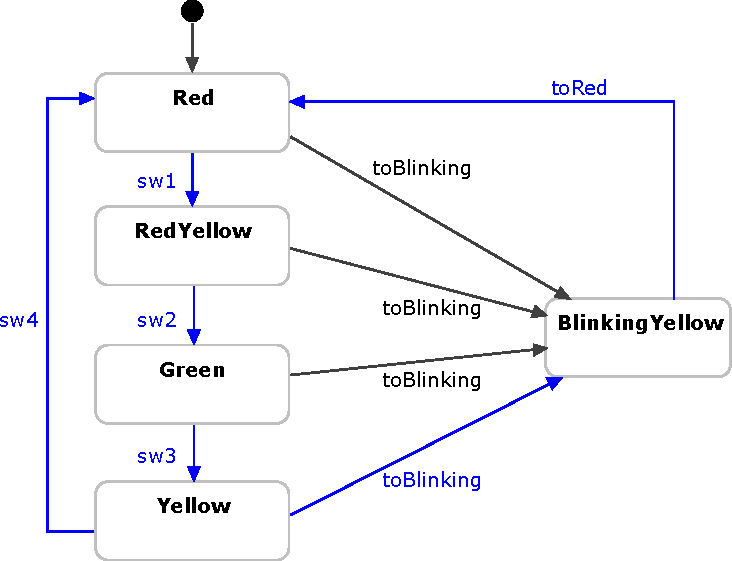
\includegraphics[scale=0.7]{modellek-ellenorzese/figures/pic_fedettseg-jelzolampa-pelda.pdf}
	\end{center}
	
Vegyük az alábbi, két tesztesetből álló tesztkészletet (az elfogadási kritérium nem lényeges a fedettség szempontjából, így azt elhagytuk):

\begin{center}
\begin{tabular}{l|ll}
Teszteset & Bemenet (\code{n}) \\ \hline
1 & \code{sw1}, \code{sw2}, \code{sw3}, \code{sw4} \\
2 & \code{sw1}, \code{sw2}, \code{sw3}, \code{toBlinking}, \code{toRed} \\
\end{tabular}
\end{center}

Ez a két teszt az összes állapotot be fogja járni. Így az állapotgépben az \emph{állapotfedettség} $\frac{5}{5} = 1 = 100 \%$.

Ugyanakkor ez a tesztkészlet mégsem érzékeny minden hibára. Nem tudnánk kimutatni például, ha az implementációban kifelejtenénk a \allapot{RedYellow}-ból \allapot{BlinkingYellow}-ba vezető tranzíciót. Ez azért van, mert bár az állapotfedettség teljes, az átmenetfedettség nem. Összesen 9 tranzíció található az állapotgépben, ebből 6-ot fed le a két teszteset együtt (kékkel jelölt átmenetek), így az \emph{átmenetfedettség} $\frac{6}{9} = 0{,}666 = 66{,}6 \%$.

Fontos megjegyezni, hogy ha elérnénk néhány új teszteset definiálásával a teljes átmenetfedettséget, az sem feltétlen lenne képes kimutatni minden lehetséges hibát. Ha például az implementációban -- hibásan -- szerepelne egy \allapot{Green} állapotból \allapot{Red} állapotba vezető átmenet, azt nem feltétlen tudnánk kimutatni egy (a specifikáción) teljes fedettséget elérő tesztkészlettel sem.
\end{pelda}

A fenti áttekintésből az is látszik, hogy egy magas fedettségi arány csak szükséges, de nem elégséges feltétele a jó minőségű rendszer fejlesztésének. Gyakran ez a szám félrevezető is lehet, illetve rossz irányba viheti a teszttervezést.


\section{Tesztelés futásidőben (futásidejű verifikáció)}\label{sec:futasideju-verifikacio}
Ebben a fejezetben a futásidejű ,,öntesztelés'' vagy monitorozás alapötletét mutatjuk be. Bizonyos esetekben kiemelkedően magas minőségi elvárásaink vannak a rendszerünkkel szemben (pl. biztonságkritikus alkalmazási területek). Más esetekben olyan külső komponenseket használunk, amelyek minőségéről nem tudunk alaposan meggyőződni (pl. egy lefordított, más által fejlesztett alkalmazást csak korlátozottan tudunk tesztelni). Ilyenkor az elvárásaink egy részét elhelyezzük magában a megvalósított rendszerben és folyamatosan vizsgáljuk. Azokat a követelményeket, amelyek teljesülését folyamatosan, minden állapotban elvárjuk, \fogalomragozva{invarians}{invariánsoknak} nevezzük.

A monitorozás általános elrendezését szemlélteti \aref{fig:monitorozas-elrendezes}.~ábra.

\begin{figure}[h]
	\centering
	\input{modellek-ellenorzese/figures/monitorozas-elrendezes.pdf_tex}
	
	\caption{A monitorozás általános elrendezése}
	\label{fig:monitorozas-elrendezes}
\end{figure}

A monitorozás két fő lépésből áll:
\begin{itemize}
\item \emph{bemenetek ellenőrzéséből}, amely során a bemeneti adatok megfelelőségét vizsgáljuk a definiált bemeneti invariánsok (előfeltételek) alapján, és/vagy
\item \emph{hihetőségvizsgálatból}, amely során a kimeneti adatok megfelelőségét vizsgáljuk a bemeneti adatok és a definiált kimeneti invariánsok (utófeltételek) alapján.
\end{itemize}

Egyes esetekben az invariánsok igen egyszerűek (például egy valós számok négyzetre emelést megvalósító függvény végén vizsgálhatjuk, hogy a kapott eredmény negatív-e; a negatív eredményt hibásnak minősítjük). Ilyenkor tipikusan az implementáció is három részre tagolódik, követve \aref{fig:monitorozas-elrendezes}.~ábrán látható elrendezést:
\begin{itemize}
\item Először az \emph{előfeltételt} vizsgáljuk. Ha ez nem teljesül, kivételről beszélünk. Ez egy normálistól eltérő, váratlan helyzet, aminek a kezelését máshol valósítjuk meg (ilyen körülmények közt az implementációnk helyességét nem követeljük meg). Ha az előfeltétel nem teljesül, annak oka a rendszer hibás használata (nem megfelelő bemeneti adatokat kapott).
\item Amennyiben az előfeltétel teljesült, megtörténik az érdemi logika \emph{végrehajtása}.
\item A végrehajtás után az utófeltétel vizsgálatára kerül sor. Amennyiben az utófeltétel nem teljesül, olyan hibás állapotba került a rendszer, amely kezelésére nincs felkészítve. Ennek oka lehet a hibás implementáció vagy futásidejű hiba.
\end{itemize}

\begin{pelda}
Az alábbi példakód egy másodfokú egyenlet gyökeit számolja ki:

\begin{lstlisting}[language=C++]
void Roots(float a, b, c, float &x1, &x2) {
    float d = sqrt(b*b-4*a*c);

    x1 = (-b+d)/(2*a);
    x2 = (-b-d)/(2*a);
}
\end{lstlisting}

Tudhatjuk, hogy ez a kód nem működik helyesen minden esetben. Feltételezzük, hogy a diszkrimináns ($D=b^2-4\cdot a\cdot c$) nemnegatív, különben a gyökvonást negatív számon végezzük el. Tudjuk azt is, hogy a kiszámított $x_1$ és $x_2$ értékeknek zérushelyeknek kell lennie, azaz elvárt, hogy $ax_1^2 + bx_1 + c = 0$ és $ax_2^2 + bx_2 + c = 0$. Ezekkel az elő- és utófeltételekkel kiegészíthetjük az implementációt is az alábbiak szerint:


\begin{lstlisting}[language=C++,morekeywords={assert}]
void RootsMonitor(float a, b, c, float &x1, &x2) {
    // el(*@\textcolor{commentcolor}{ő}@*)feltétel
    float D = b*b-4*a*c;
    if (D < 0)
        throw "Invalid input!";

    // végrehajtás
    Roots(a, b, c, x1, x2);

    // utófeltétel
    assert(a*x1*x1+b*x1+c == 0 && a*x2*x2+b*x2+c == 0);
}
\end{lstlisting}
\end{pelda}

Monitorozást nem csak ilyen egyszerű esetekben lehet használni, összetett monitorok is elképzelhetők. Például állapotgépek esetén készíthetünk egy monitor régiót, ami a rendszer megvalósításával párhuzamosan fut és detektálja a hibás vagy tiltott állapotokat, akciókat.







\section{Formális verifikáció\kieg}\label{sec:formalis-verifikacio}
\Fogalom{formalis-verifikacio} alatt olyan módszereket értünk, amelyek segítségével adott modellek vagy programok helyességét matematikailag precíz eszközökkel vizsgálhatjuk. Három fontosabb formális verifikációs módszert (családot) említünk meg:
\begin{itemize}
\item Modellellenőrzés;
\item Automatikus helyességbizonyítás, amely során axiómarendszerek alapján tételbizonyítás segítségével próbáljuk a helyességet belátni;
\item Konformanciavizsgálat, amely során adott modellek közt bizonyos konformanciarelációk teljesülését vizsgáljuk, így beláthatjuk, hogy különböző modellek viselkedése megegyező vagy eltérő az adott relációk szerint.
\end{itemize}

Jelen jegyzetben kitekintésként a modellellenőrzést mutatjuk be röviden. Bővebben a formális verifikációról a \form (BMEVIMIM100) MSc tárgy\footnote{\url{https://inf.mit.bme.hu/edu/courses/form}} keretei közt szólunk.

\paragraph{Modellellenőrzés.}
A \fogalom{modellellenorzes} egy olyan módszer, amelynek során egy adott modellen vagy implementáción egy követelmény teljesülését vizsgáljuk. A modellellenőrzés egyik előnye, hogy amennyiben a követelmény nem teljesül, lehetséges egy ellenpéldát adni. Az \fogalom{ellenpelda} egy olyan futási szekvencia, amely megmutatja, hogyan lehetséges a vizsgált követelményt megsérteni. Ez nagyban segíthet a hibás működés okának meghatározásában.

A modellellenőrzés -- a teszteléssel szemben -- egy \emph{teljes} módszer, azaz az adott modell vizsgálata kimerítő. Ennek következtében lehetőség van a helyes működés bizonyítására is, míg ez teszteléssel nem lehetséges. Ugyanakkor a modellellenőrzés igen nagy számítási igényű, ezért használhatósága korlátozott.



\section{Kapcsolódó témák}
\textbf{TODO}

\section{Gyakorlati jelentőség}
Mint azt már a fejezet elején említettük, az informatikának, mint mérnöki diszciplínának kulcsfontosságú része az elkészített munka ellenőrzése, legyen az specifikáció vagy implementáció. Minél nagyobb az elkészített rendszer kritikussága, annál nagyobb a fejlesztés folyamán az ellenőrzése szerepe.

Manapság már szinte elképzelhetetlen egy modern fejlesztőkörnyezet beépített statikus ellenőrzés nélkül. Elérhetők további, igen kifinomult eszközök, amelyek statikus ellenőrzés segítségével felhívhatják a figyelmet hibákra vagy veszélyes konstrukciókra. 

Az általunk írt implementáció nem tekinthető befejezettnek, amíg nem terveztünk és implementáltunk hozzá egy megfelelő tesztkészletet. Természetesen nem csak a megfelelően releváns tesztkészlet megvalósítása az elvárás: az implementációnkon a teszteknek sikeresnek kell lenniük ahhoz, hogy a fejlesztés következő fázisára továbbléphessünk, legyen az akár az integráció, akár a megrendelőnek történő átadás.

Különösen kritikus esetekben, például egy repülő vagy egy atomerőmű vezérlőrendszerénél, netán orvosi eszközök beágyazott szoftvereinél a tesztelés ismertetett hibái túlzott kockázatot hordozhatnak, ezért gyakran kiegészül a tervek és a megvalósítás vizsgálata formális módszerek használatával.

\subsection{Kapcsolódó eszközök}
Ebben a szakaszban néhány olyan (többnyire jól ismert és ingyenes) eszközt sorolunk fel, amely a gyakorlatban megvalósítja a bemutatott módszerek némelyikét.

Egyszerűbb statikus analízis eszközöket beépítve találhatunk a fejlettebb fejlesztőeszközökben (pl. Eclipse\footnote{\url{http://eclipse.org}}) és modellező eszközökben (pl. Yakindu). Ezeken kívül számos, mélyebb analízist lehetővé tevő eszköz létezik. C esetén gyakran használatos a Lint stb. nyelv esetén a Cppcheck\footnote{\url{http://cppcheck.sourceforge.net/}} és cpplint\footnote{\url{https://github.com/google/styleguide/tree/gh-pages/cpplint}} eszközök. Java nyelvű programok statikus ellenőrzésére használható például a FindBugs\footnote{\url{http://findbugs.sourceforge.net/}} vagy a PMD\footnote{\url{http://pmd.github.io/}} eszköz. A Coverity cég C, \cpp és Java nyelvű programok statikus ellenőrzésére kínál megoldást, amelyek közül például a Coverity Scan\footnote{http://www.coverity.com/products/coverity-scan/} nyílt forráskódú programokra ingyenesen használható.

C és \cpp nyelvű programokhoz használható tesztfuttató keretrendszer például a Google Test\footnote{\url{https://github.com/google/googletest}}. Java programok modultesztelését segítheti például a JUnit\footnote{\url{http://junit.org/}} keretrendszer.

C és \cpp nyelvű szoftverek modellellenőrzésre jól használható például a CBMC\footnote{\url{http://www.cprover.org/cbmc/}} eszköz. ,,Állapotgép-jellegű'' modellek esetén jó választás lehet az UPPAAL\footnote{\url{http://www.uppaal.org/}} vagy a nuXmv\footnote{\url{https://nuxmv.fbk.eu/}} eszközök használata.

\section{Tanulást segítő anyagok}

\subsection{Ellenőrző kérdések}
\begin{itemize}
	\item  \textbf{TODO}
	\item
	\item
\end{itemize}

%\subsection{Kulcsfogalmak}
%\textbf{TODO}

%\subsection{Szójegyzék}
%\textbf{TODO}
% !TeX spellcheck = hu_HU
\topic{Vizuális adatelemzés}

%\section{Jegyzet}

Jegyzetként kérjük használják az ,,Intelligens adatelemzés'' c. könyv 5. fejezetét (\emph{Vizuális analízis}). Elérhető a \url{http://docs.inf.mit.bme.hu/remo-jegyzet/vizualis-adatelemzes-konyvfejezet.pdf} címen, ill. ingyenesen megvásárolható a \url{http://www.interkonyv.hu/konyvek/antal_peter_intelligens_adatelemzes} címen.

%\section{Kiegészítő anyagok\kieg}
%
%\subsection{Valószínűségszámítási alapfogalmak}
%
%\begin{definicio}
%	\begin{itemize}
%		\item \Fogalom{valoszinusegi-valtozo} (\fogalom{valoszinusegi-valtozo}): $X$
%		\item \Fogalom{varhato-ertek}, \fogalom{atlag} (\fogalomangolul{varhato-ertek}, \fogalomangolul{atlag}):
%		$$\mu = \mathbb{E}X = \sum_{i=1}^{n} p_i x_i$$
%
%		\item \Fogalom{szorasnegyzet} (\fogalomangolul{szorasnegyzet}):
%
%		$$\sigma^2 = \mathbb{E}\left(X-\mu\right)^2 = \sum_{i=1}^{n} p_i (x_i - \mu)^2$$
%
%		\item \Fogalom{szoras} (\fogalomangolul{szoras}):
%
%		$$\sigma = \sqrt{\mathbb{E}\left(X-\mu\right)^2} = \sqrt{\sum_{i=1}^{n} p_i (x_i - \mu)^2}$$
%	\end{itemize}
%\end{definicio}
%
%\subsection{Statisztikai alapfogalmak}
%
%\begin{definicio}
%	\begin{itemize}
%		\item \fogalomragozva{megfigyeles}{Megfigyelések}: $t$ darab, $x_1, \dots, x_t$
%		\item \Fogalom{tapasztalati-atlag} (\fogalomangolul{tapasztalati-atlag}):
%
%		$$m = \bar{x} = \frac{x_1 + \dots + x_t}{t}$$
%
%		\item \Fogalom{korrigalt-tapasztalati-szoras} (\fogalomangolul{korrigalt-tapasztalati-szoras}):
%
%		$$s = \sqrt\frac{\left(x_1-m\right)^2 + \dots + \left(x_t-m\right)^2}{t-1} = \sqrt\frac{\sum_{i=1}^{t}\left(x_i - m\right)^2}{t-1}$$
%
%		Figyeljük meg, hogy a korrigált tapasztalati értékeknél $t$ helyett $(t-1)$-gyel osztunk. Ennek oka, hogy $t$-vel osztva a kapott érték általában alábecsli a teljes populáció szórását. Belátható, hogy $(t-1)$-gyel osztva a valódi szórást jobban közelítő értéket kapunk. Ezt nevezzük Bessel-féle korrekciónak (\url{https://en.wikipedia.org/wiki/Bessel's\_correction}).
%	\end{itemize}
%\end{definicio}
%
%\subsection{Kísérlettervezés}
%
%A \fogalomragozva{CLT}{centrális határeloszlás-tételből} (\roviditesangolul{CLT}) következőik, hogy tetszőleges eloszlású jellemző (véges $m$ várható értékkel és $s$ szórással) tapasztalati átlaga $t \rightarrow \infty$ esetén normális eloszlású, $\mu = m$ várható értékkel és $\sigma = \frac{s}{\sqrt{t}}$ szórással.
%
%Ökölszabály: ismert szórásnál $t > 30$, ismeretlen szórásnál $t > 100$ után kezd elfogadható lenni a közelítés.
%
%A normális eloszlású változó
%\begin{itemize}
%	\item az esetek 68\%-ában legfeljebb $1\sigma$ messze kerül $\mu$-től,
%	\item az esetek 95\%-ában legfeljebb $2\sigma$ messze kerül $\mu$-től,
%	\item az esetek 99,7\%-ában legfeljebb $3\sigma$ messze kerül $\mu$-től.
%\end{itemize}
%
%\remofigscale{felderito-adatelemzes/gaussian-distribution}{Konfidenciaintervallumok}{0.3}

% !TeX spellcheck = hu_HU
\topic{Benchmarking}\label{cha:benchmarking}

\graphicspath{ {./benchmarking/figures/} }

%\todo[inline]{ez a fejezet elég jó, leginkább ábra kellene bele}

\section{Alapfogalmak}

Motiváció
 Szoftver/hardver eszközök teljesítményének 
összehasonlítása
 Döntéstámogatás 
o Melyiket előnyösebb megvenni/telepíteni?
o Mekkora terhelésre elég a meglévő rendszer?
 Teljesítménytesztelés 
o Kell‐e még a teljesítményen javítani és hol 
(fejlesztésnél)?
o Optimális‐e egy konkrét beállítás?
o Van‐e egy beállításnak teljesítményre gyakorolt hatása 
(érzékenység vizsgálat)?

Fejlesztés alatt lévő rendszer
 Teljesítmény felmérése
o Modell alapján becsült értékek
o Megvalósított rendszer értékei „éles” helyzetben
 Tervezői és menedzsment döntések
o Melyik részébe fektessünk több energiát (≈ pénzt)? 
 Mi alapján döntsünk?
o Jelenlegi erősségek és gyengeségek
 Mi számít erősségnek vagy gyengeségnek?
o Mire képesek a hasonló rendszerek, versenytársak?

Elkészített rendszer
 Versenyképesség felmérése
o Versenytársak eredményei
 Marketing stratégiák
o Miért minket válasszanak?
 Milyen adatokra hivatkozzunk?
o A miénk a legjobb rendszer egy esettanulmány szerint
• És a többi esetben?
o Ki rangsorolta az elérhető rendszereket?
o Mi alapján?

\begin{definicio}
	A \fogalom{benchmarkolas}
	\begin{itemize}
		\item egy \emph{program} (programok, vagy más műveletek) \emph{futtatása},
		\item \emph{szabványos tesztekkel} vagy bemenetekkel,
		\item egy objektum \emph{relatív teljesítményének} felmérése érdekében.
	\end{itemize}
\end{definicio}

A Wikipédia definíciója~\cite{wiki:benchmark} (kiemelések a jegyzet szerzőitől):

\begin{quote}
	In \textbf{computing}, a benchmark is the \textbf{act of running} a computer program, a set of programs, or other operations, in order to \textbf{assess the relative performance} of an object, normally by running a number of \textbf{standard tests} and trials against it.
\end{quote}

Elvárások
 Ismételhetőség (Repeatability)
o Egy elemen többször megismételt mérés/művelet
eredményeinek változékonysága (szóródási faktor)
 Reprodukálhatóság (Reproducibility)
o A mérési rendszer változékonysága, amelyet a 
műveletek viselkedéseinek különbsége okoz
 Általánosított felhasználói eset
o Átlag felhasználó számára értelmezhető legyen az
eredmény
Szabványok/megállapodások betartása
 Relevancia
o Tényleg azt az alkalmazást mérjük, amit kell
o Terhelésgenerálás jellege közelítse a valódi terhelést
o Minimalizáljuk a zavaró tényezőket
• Memória cache tartalma
• Betöltött/kilapozott memória területek
• Diszk cache tartalma


~\cite{DBLP:books/mk/Gray93}



\section{Benchmarkok\kieg}

PassMark

\rovidites{SPEC} (\roviditesangolulkifejtve{SPEC})

\rovidites{TPC} (\roviditesangolulkifejtve{TPC})

\rovidites{TPCC}


% !TeX spellcheck = hu_HU
\topic{Kódgenerálás}


\bibliographystyle{bib/huplain}
\bibliography{bib/remo}	
\irodalomjegyzektartalomjegyzekbe

\IfFileExists{./use-xindy}{
	\printglossary[title=Tárgymutató]
}{
	\printnoidxglossary[title=Tárgymutató]
}


\end{document}
